\documentclass[xcolor=dvipsnames,aspectratio=1610]{beamer}

\usepackage{graphicx}
\usepackage[scale=2]{ccicons}
\usepackage{multicol}
\usepackage{enumitem}
\usepackage{xcolor}
\usepackage{algorithm, caption}
\usepackage[noend]{algpseudocode}
\usepackage[absolute,overlay]{textpos}
\usepackage{calc}
\usepackage[backend=bibtex,citestyle=authortitle]{biblatex}
\usepackage[no-math]{fontspec}

% \usepackage[texcoord,grid,gridunit=mm,gridcolor=red!10,subgridcolor=green!10]
% {eso-pic}

\setitemize{label=\usebeamerfont*{itemize item}%
  \usebeamercolor[fg]{itemize item}
  \usebeamertemplate{itemize item}}

\newcommand{\exampleheight}{1.9cm}
\newcommand{\examplewidth}{16cm}

% \makeatletter
% \newcommand{\algcolor}[2]{%
%   \hskip-\ALG@thistlm\colorbox{#1}{\raisebox{0pt}[0.1cm][0cm]{\parbox{\dimexpr\linewidth-2\fboxsep}{\hskip\ALG@thistlm\relax #2}}}%
% }
% \newcommand{\algemph}[1]{\algcolor{Yellow}{#1}}
% \makeatother

\usepackage{tikz}
\usetikzlibrary{calc}

\makeatletter
% code borrowed from Andrew Stacey; See
% http://tex.stackexchange.com/a/50054/3954
\tikzset{%
  remember picture with id/.style={%
    remember picture,
    overlay,
    save picture id=#1,
  },
  save picture id/.code={%
    \edef\pgf@temp{#1}%
    \immediate\write\pgfutil@auxout{%
      \noexpand\savepointas{\pgf@temp}{\pgfpictureid}}%
  },
  if picture id/.code args={#1#2#3}{%
    \@ifundefined{save@pt@#1}{%
      \pgfkeysalso{#3}%
    }{
      \pgfkeysalso{#2}%
    }
  }
}

\def\savepointas#1#2{%
  \expandafter\gdef\csname save@pt@#1\endcsname{#2}%
}

\def\tmk@labeldef#1,#2\@nil{%
  \def\tmk@label{#1}%
  \def\tmk@def{#2}%
}

\tikzdeclarecoordinatesystem{pic}{%
  \pgfutil@in@,{#1}%
  \ifpgfutil@in@%
    \tmk@labeldef#1\@nil
  \else
    \tmk@labeldef#1,(0pt,0pt)\@nil
  \fi
  \@ifundefined{save@pt@\tmk@label}{%
    \tikz@scan@one@point\pgfutil@firstofone\tmk@def
  }{%
  \pgfsys@getposition{\csname save@pt@\tmk@label\endcsname}\save@orig@pic%
  \pgfsys@getposition{\pgfpictureid}\save@this@pic%
  \pgf@process{\pgfpointorigin\save@this@pic}%
  \pgf@xa=\pgf@x
  \pgf@ya=\pgf@y
  \pgf@process{\pgfpointorigin\save@orig@pic}%
  \advance\pgf@x by -\pgf@xa
  \advance\pgf@y by -\pgf@ya
  }%
}

\makeatother
% end of Andrew's code

% main command to draw the colored background
\newcounter{mymark}
\newcommand\ColorLine{%
  \stepcounter{mymark}%
  \tikz[remember picture with id=mark-\themymark,overlay] {;}%
  \begin{tikzpicture}[remember picture,overlay]%
    \filldraw[Yellow]%
   let \p1=(pic cs:mark-\themymark),
   \p2=(current page.east)  in
   ([xshift=-0.3em,yshift=-0.7ex]0,\y1)  rectangle ++([xshift=-8.26cm]\x2,\baselineskip);
  \end{tikzpicture}%
}%


% colored loops and declarations
\makeatletter
\algnewcommand\CREQUIRE{\item[\ColorLine\algorithmicrequire]}%
\algnewcommand\CENSURE{\item[\ColorLine\algorithmicensure]}%
\algnewcommand\CSTATE{\State\ColorLine}%
\algnewcommand\CSTATEx{\Statex\ColorLine}%
\algnewcommand\CCOMMENT{\Comment\ColorLine}%

% \algdef{SE}[WHILE]{CWhile}{EndWhile}%
%    [2][default]{\ColorLine\algorithmicwhile\ #2\ \algorithmicdo\ALG@compatcomm{#1}}%
%    {\algorithmicend\ \algorithmicwhile}%
 \algdef{SE}[WHILE]{CWhile}{EndWhile}[1]{\ColorLine\algorithmicwhile\ #1\ \algorithmicdo}{\algorithmicend\ \algorithmicwhile}%

% \algdef{SE}[FOR]{CFOR}{ENDFOR}%
%    [2][default]{\ColorLine\algorithmicfor\ #2\ \algorithmicdo\ALG@compatcomm{#1}}%
%    {\algorithmicend\ \algorithmicfor}%
% \algdef{S}[FOR]{CFORALL}%
%    [2][default]{\ColorLine\algorithmicforall\ #2\ \algorithmicdo\ALG@compatcomm{#1}}%

\algdef{SE}[FOR]{For}{EndFor}[1]{\algorithmicfor\ #1\ \algorithmicdo}{\algorithmicend\ \algorithmicfor}%

\algdef{S}[FOR]{CForAll}[1]{\ColorLine\algorithmicforall\ #1\ \algorithmicdo}%

\algdef{SE}[LOOP]{CLOOP}{ENDLOOP}%
   [1][default]{\ColorLine\algorithmicloop\ALG@compatcomm{#1}}%
   {\algorithmicend\ \algorithmicloop}%
\algdef{SE}[REPEAT]{CREPEAT}{UNTIL}%
   [1][default]{\ColorLine\algorithmicrepeat\ALG@compatcomm{#1}}%
   [1]{\algorithmicuntil\ #1}%
\algdef{SE}[IF]{CIF}{ENDIF}%
   [2][default]{\ColorLine\algorithmicif\ #2\ \algorithmicthen\ALG@compatcomm{#1}}%
   {\algorithmicend\ \algorithmicif}%
\algdef{C}[IF]{IF}{CELSIF}%
   [2][default]{\ColorLine\algorithmicelse\ \algorithmicif\ #2\ \algorithmicthen\ALG@compatcomm{#1}}%
\algdef{Ce}[ELSE]{IF}{CELSE}{ENDIF}%
   [1][default]{\ColorLine\algorithmicelse\ALG@compatcomm{#1}}%
\makeatother
\algtext*{EndWhile}%
\algtext*{EndFor}%


\usetheme[numbering=counter, progressbar=frametitle, sectionpage=none]{metropolis}
\setbeamercolor{background canvas}{bg=white}
\setbeamertemplate{caption}{\raggedright\insertcaption\par}

\setsansfont[ItalicFont={Fira Sans Light Italic},%
             BoldFont={Fira Sans Bold},%
             BoldItalicFont={Fira Sans Italic}]%
            {Fira Sans Light}

\title{Conflict-Free Vertex Coloring of Planar Graphs}
\date{April 15, 2017}
\author{Shawn Seymour}

\begin{document}
  \maketitle

  \begin{frame}
    \begin{figure}[h]
      \centering
      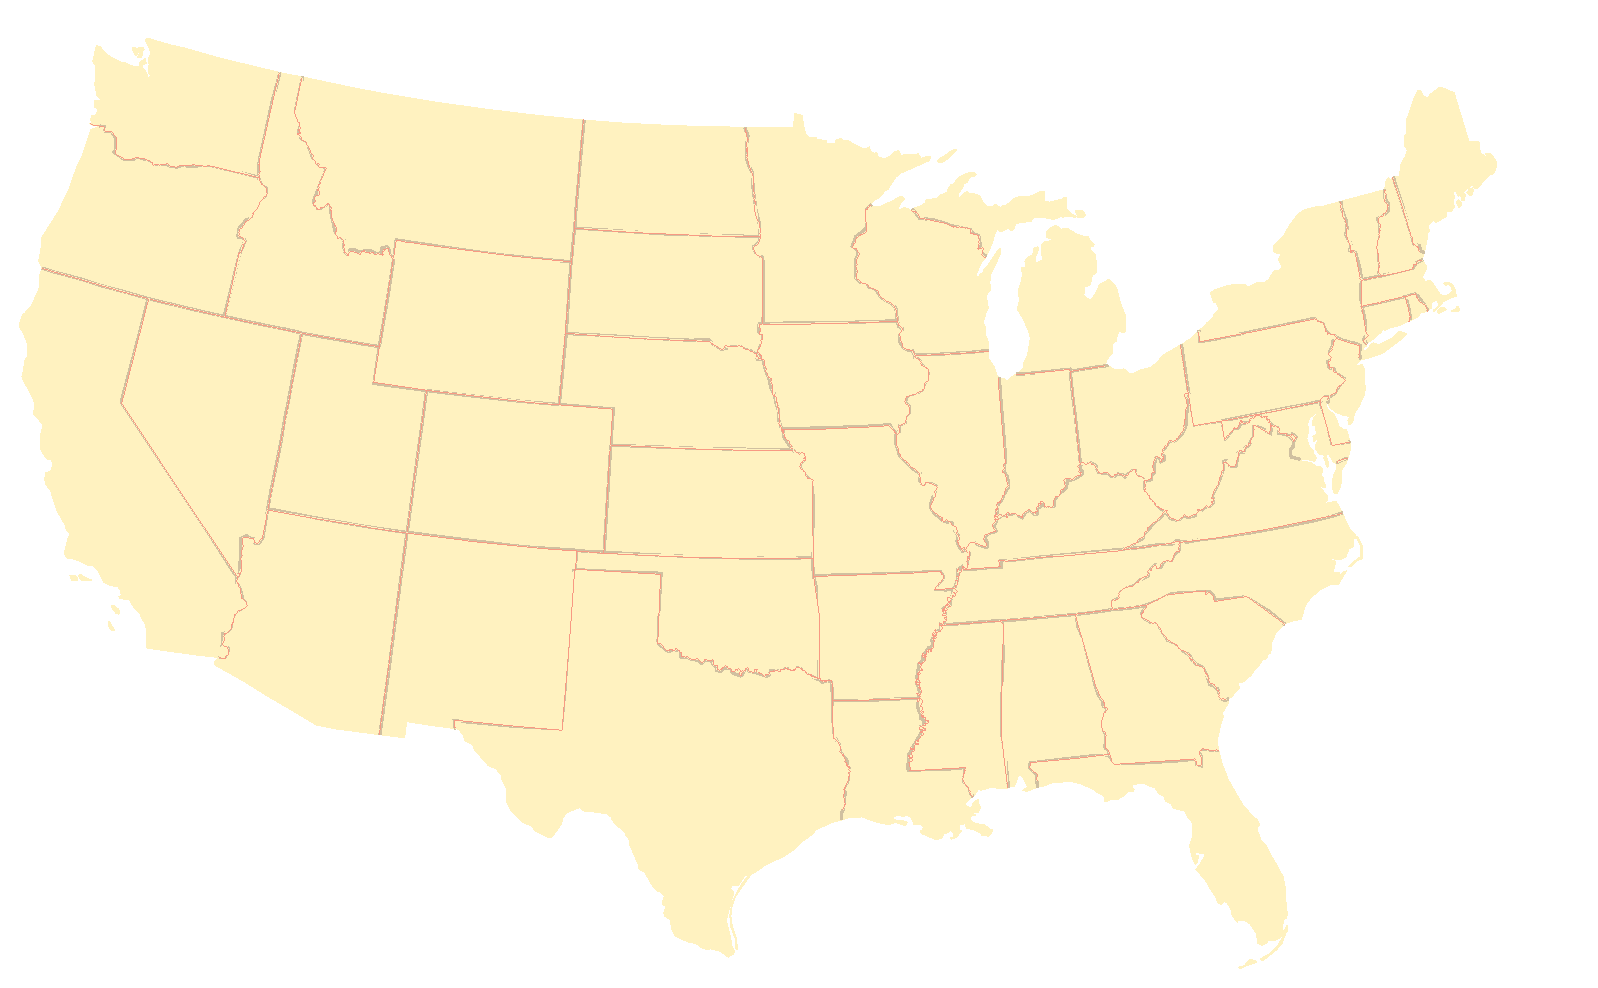
\includegraphics[width=14cm]{../figures/map-no-colors-1.pdf}
    \end{figure}
  \end{frame}

  \begin{frame}
    \begin{figure}[h]
      \centering
      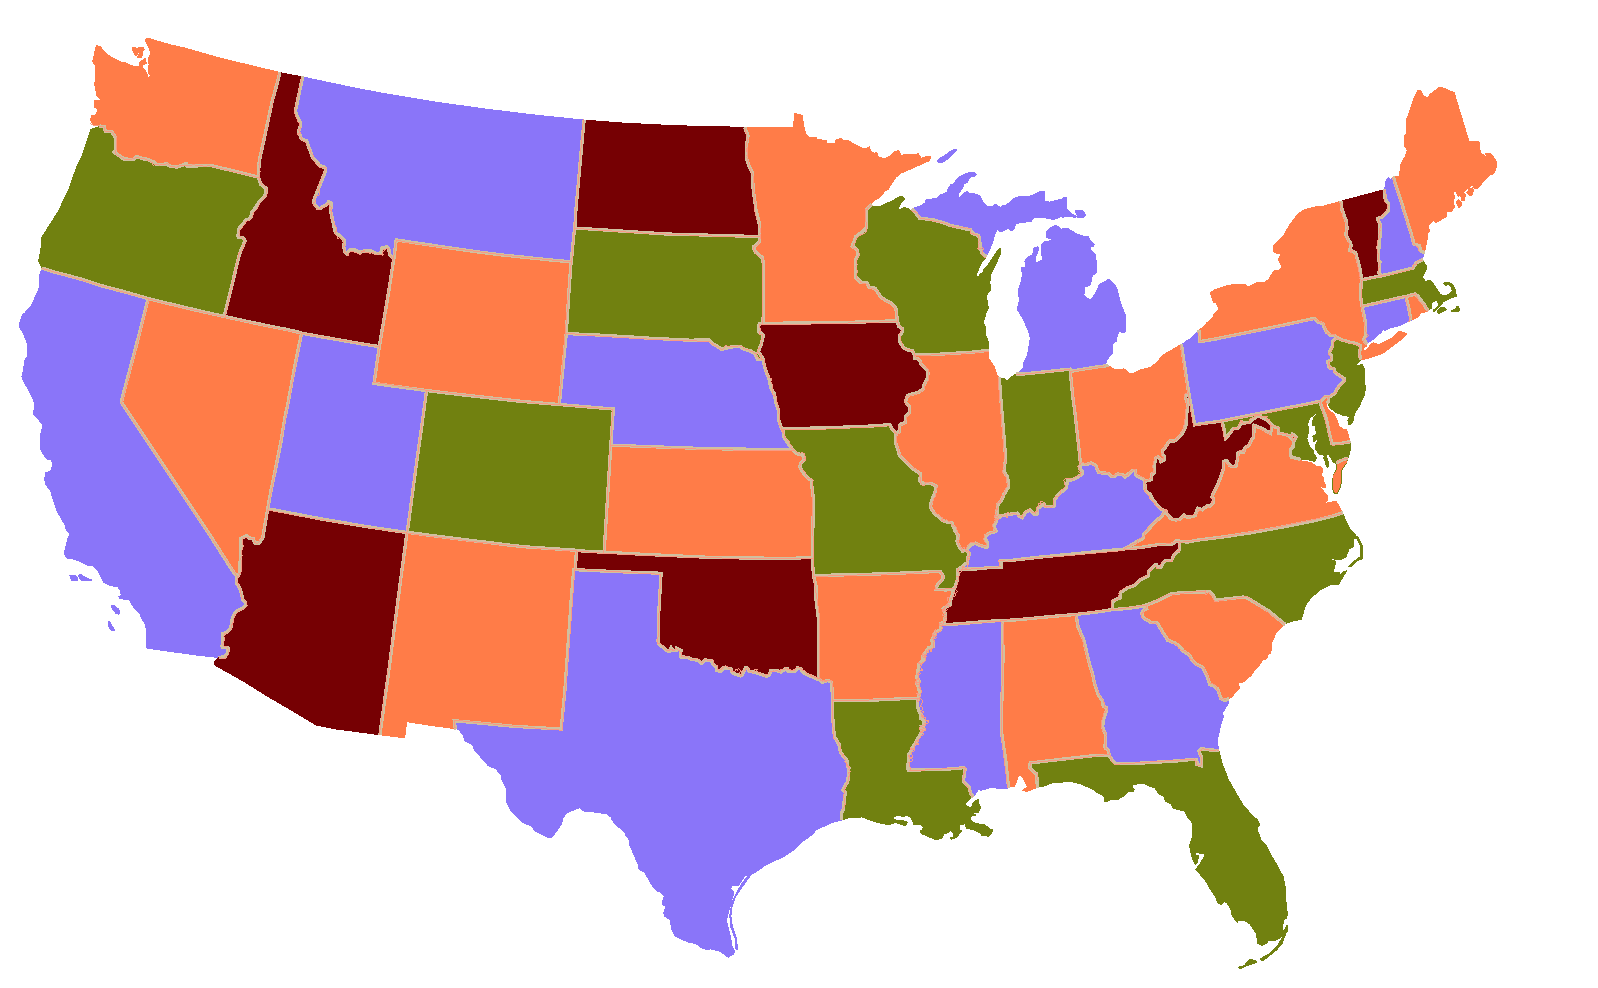
\includegraphics[width=14cm]{../figures/map-colors.pdf}
    \end{figure}
  \end{frame}

  \begin{frame}
    \frametitle{Overview}
    \begin{multicols}{2}
      \tableofcontents
    \end{multicols}
  \end{frame}

  \addtocontents{toc}{\protect\vspace{-14pt}}

  \section{Background}

  \subsection{Graph Theory}

  \begin{frame}
    \frametitle{Graph Theory}



    \only<1-3,6,9,11>{
      \begin{textblock*}{\examplewidth}(0cm,\exampleheight) % {block width} (coords)
        \centering
        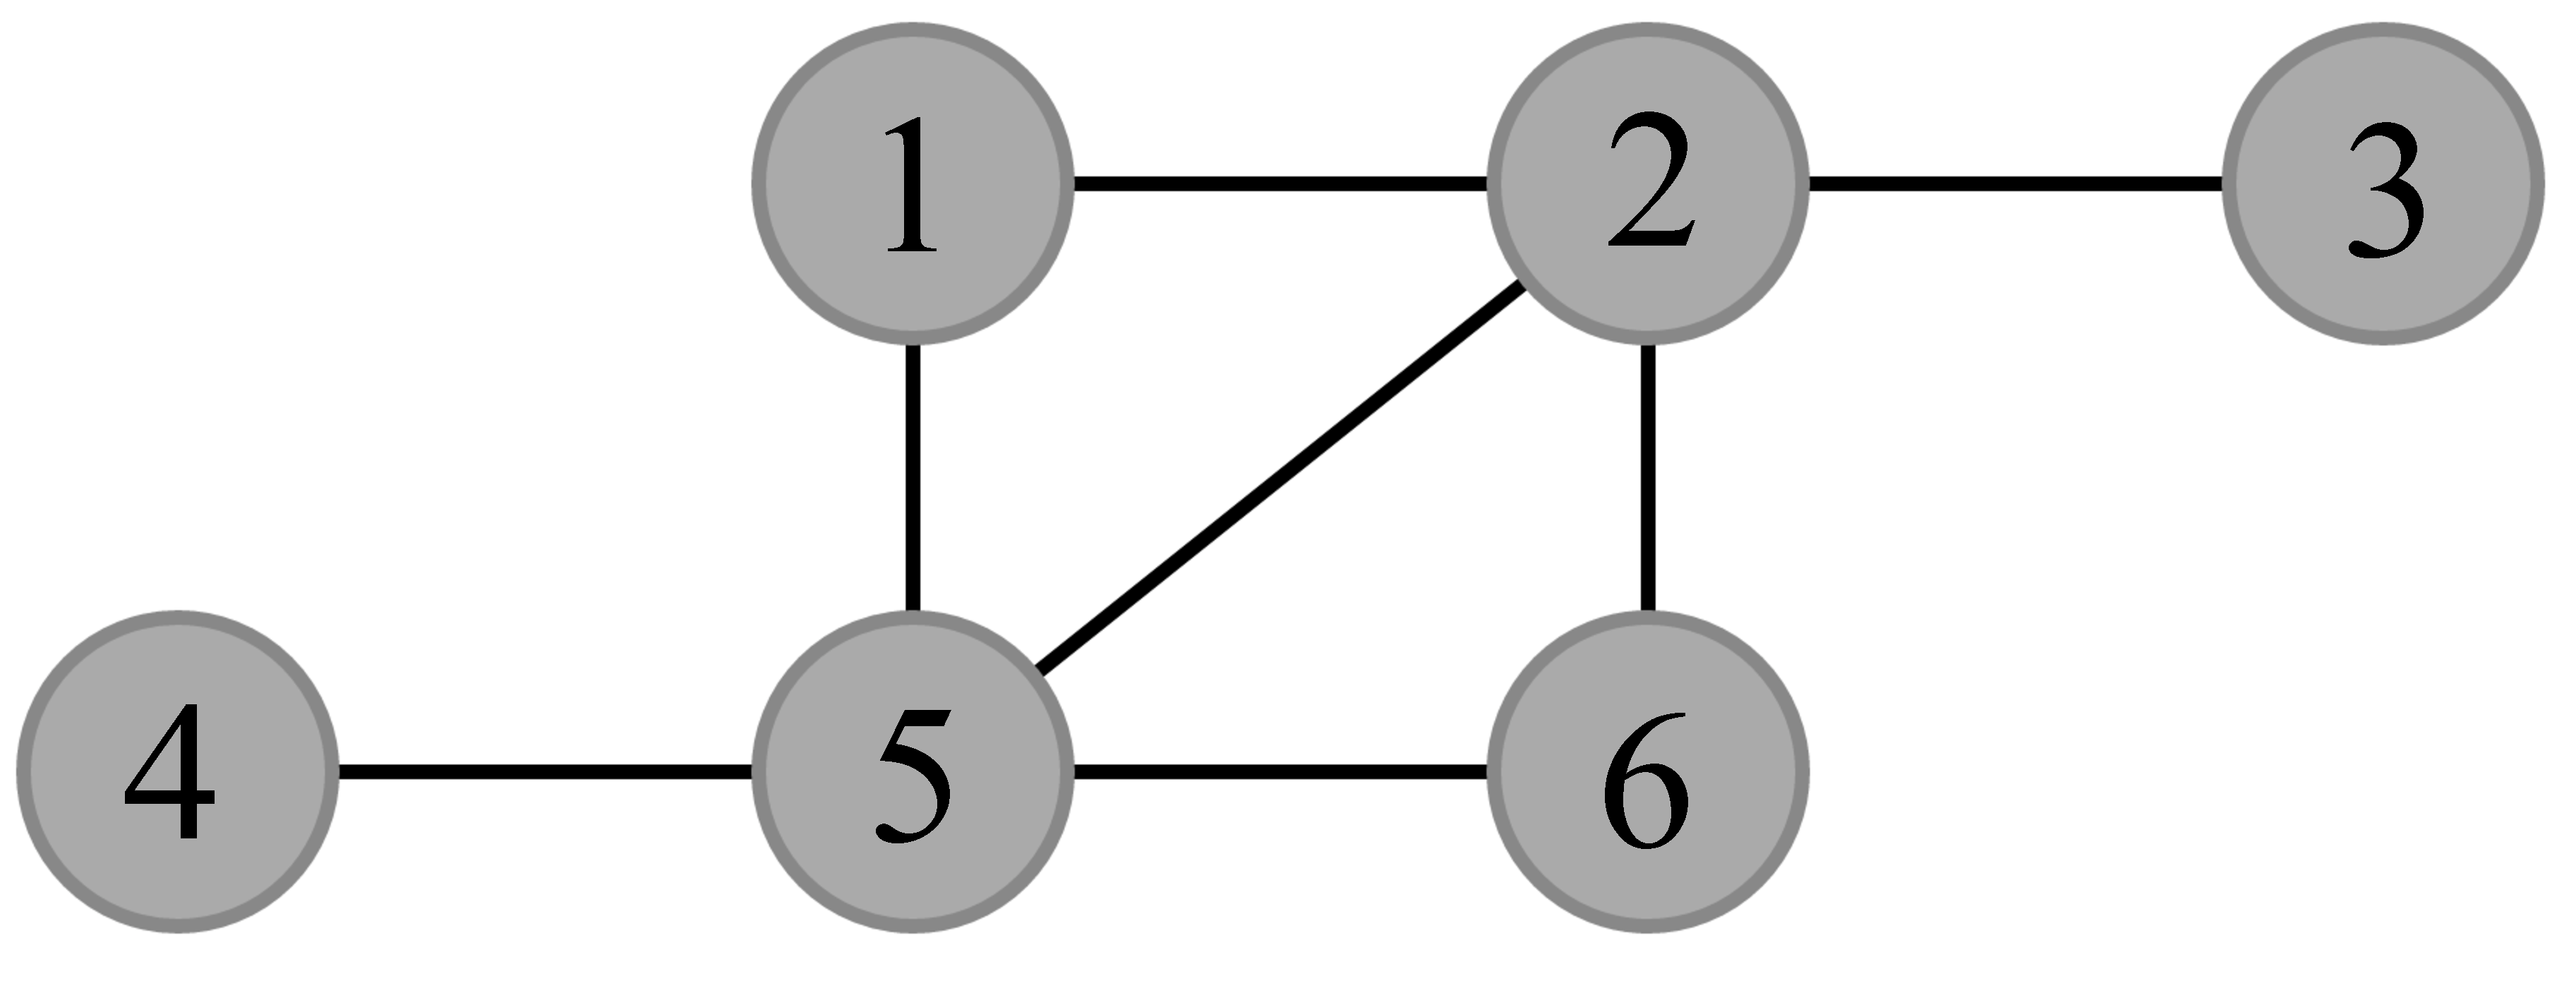
\includegraphics[width=8cm]{../figures/example.pdf}
      \end{textblock*}
    }

    \only<4> {
      \begin{textblock*}{\examplewidth}(0cm,\exampleheight) % {block width} (coords)
        \centering
        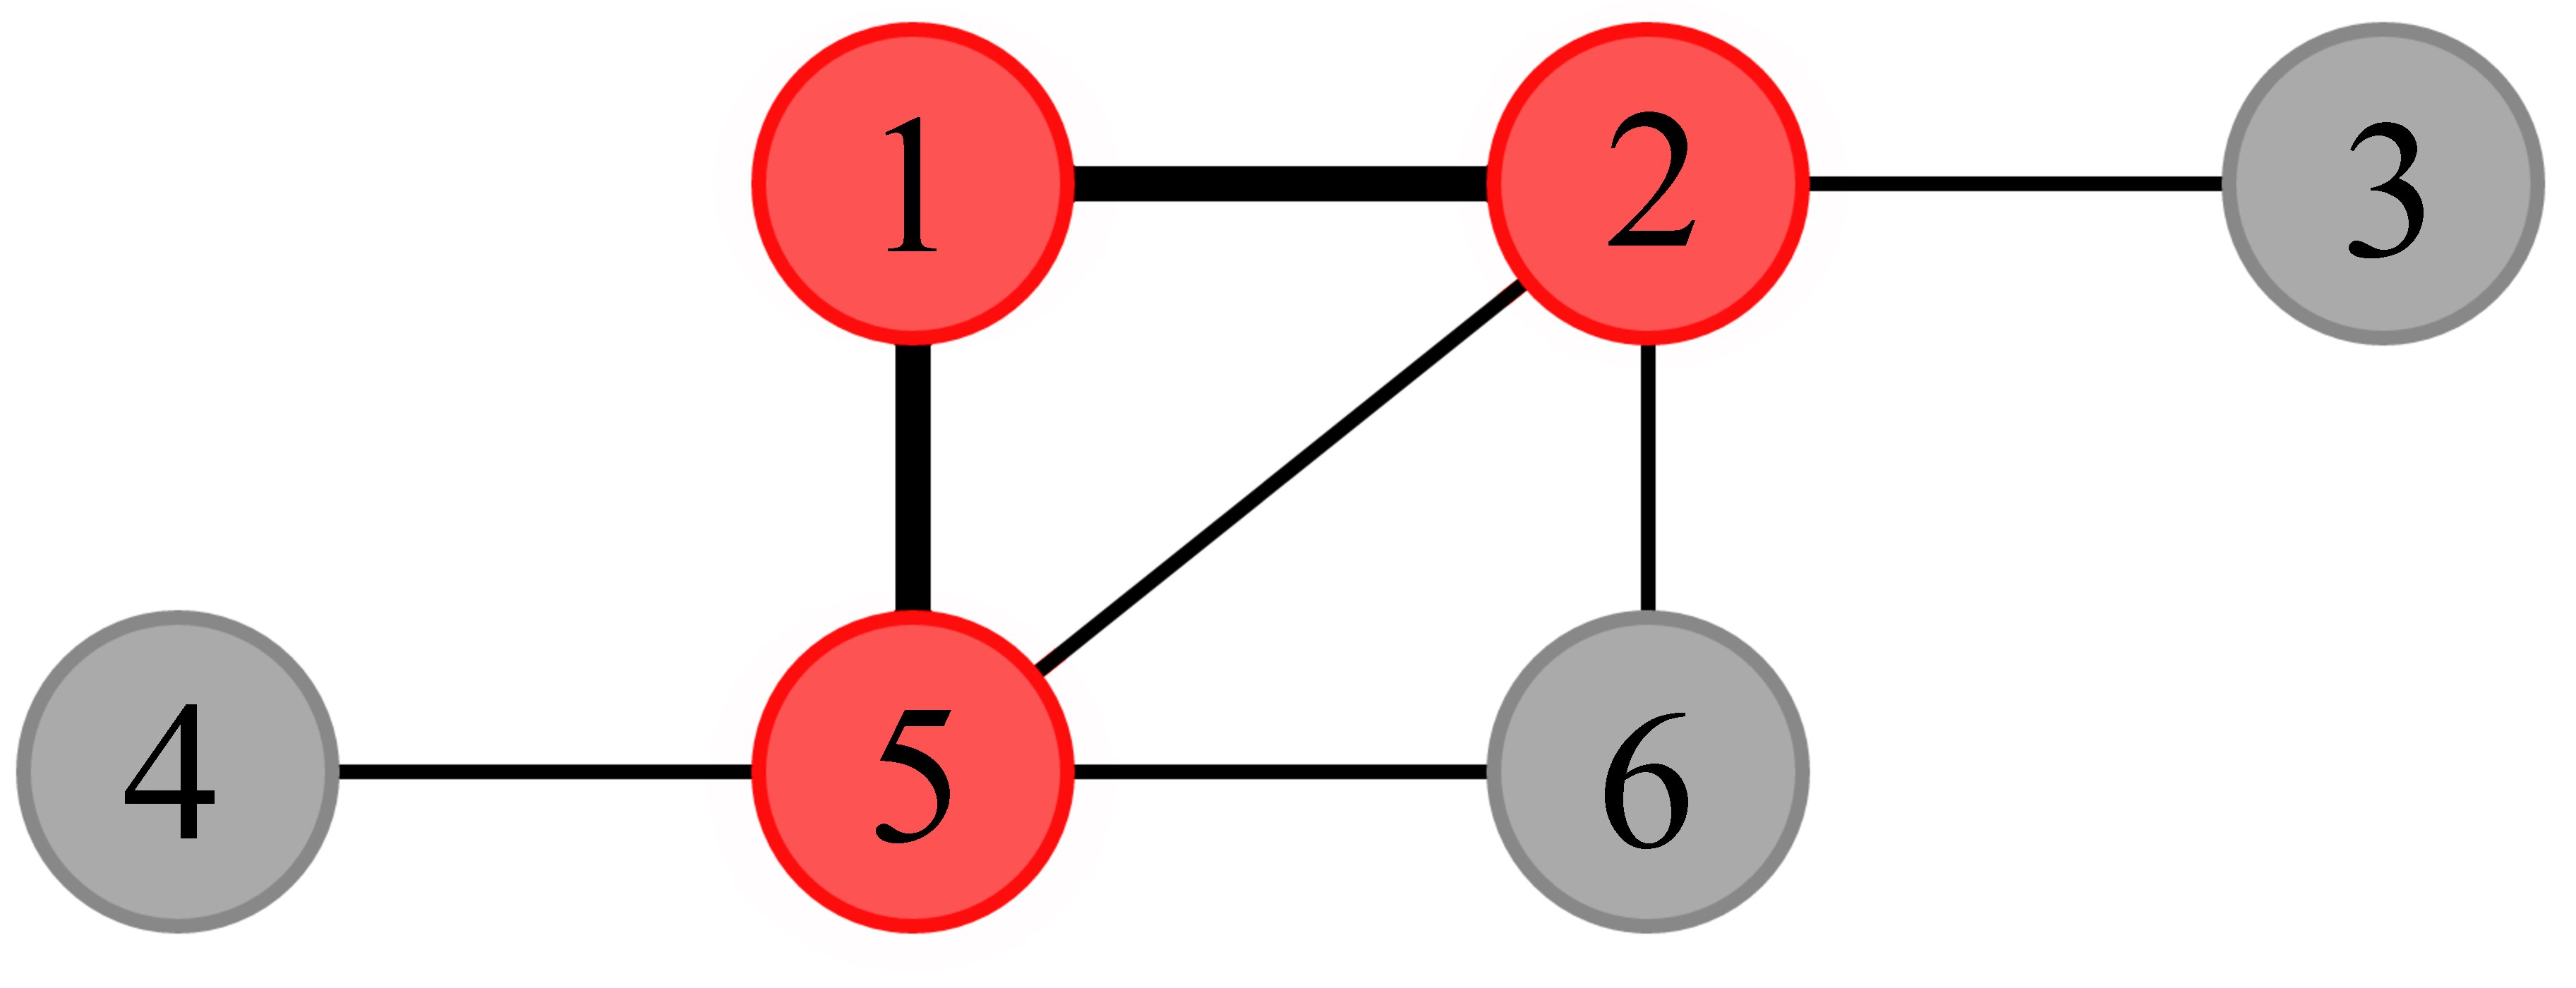
\includegraphics[width=8cm]{../figures/example-neighborhoods-1.pdf}
      \end{textblock*}
    }

    \only<5> {
      \begin{textblock*}{\examplewidth}(0cm,\exampleheight) % {block width} (coords)
        \centering
        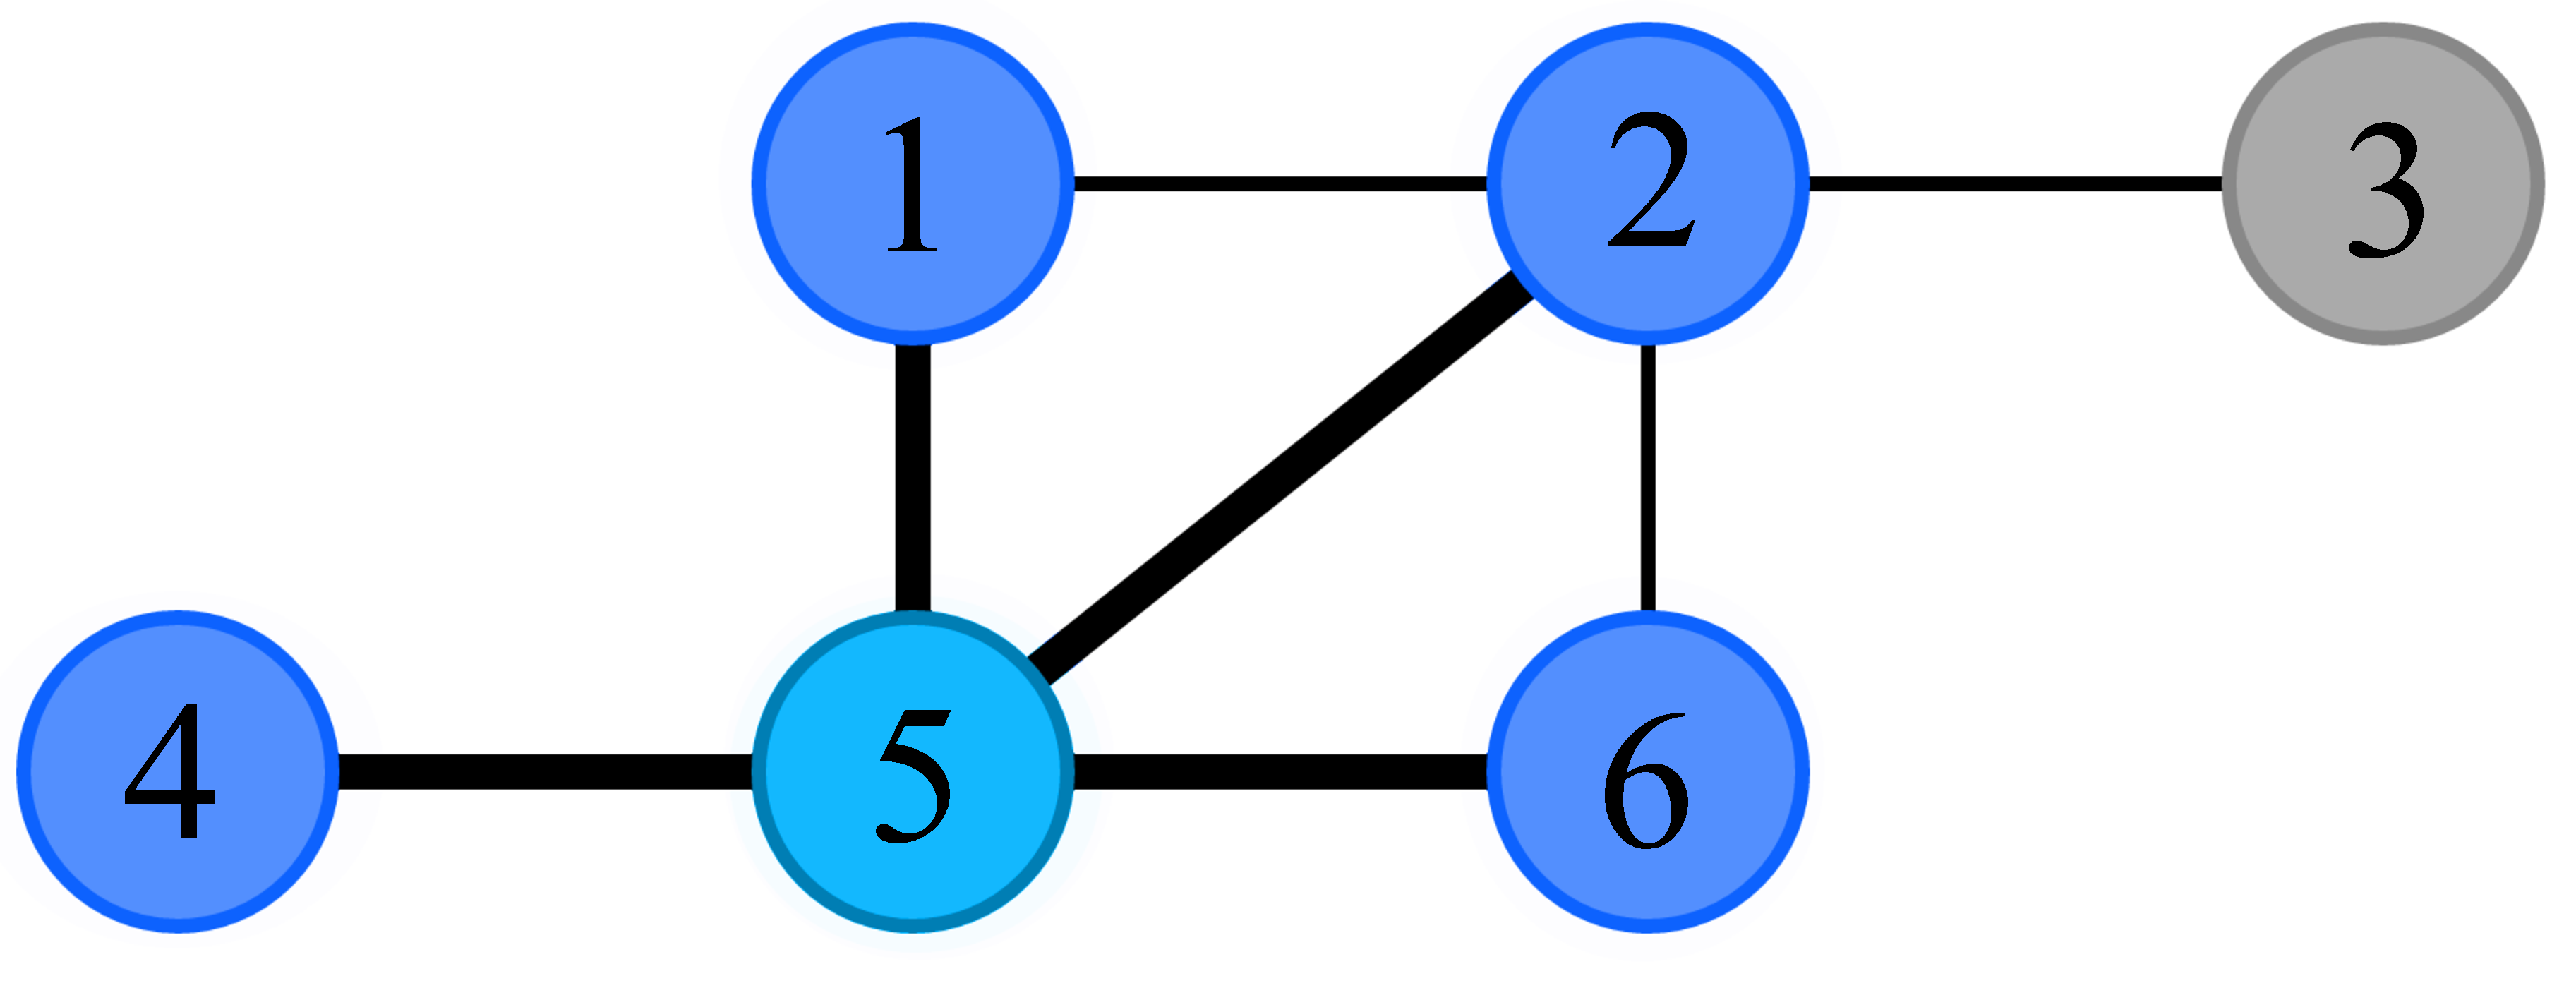
\includegraphics[width=8cm]{../figures/example-neighborhoods-2.pdf}
      \end{textblock*}
    }

    \only<7> {
      \begin{textblock*}{\examplewidth}(0cm,\exampleheight) % {block width} (coords)
        \centering
        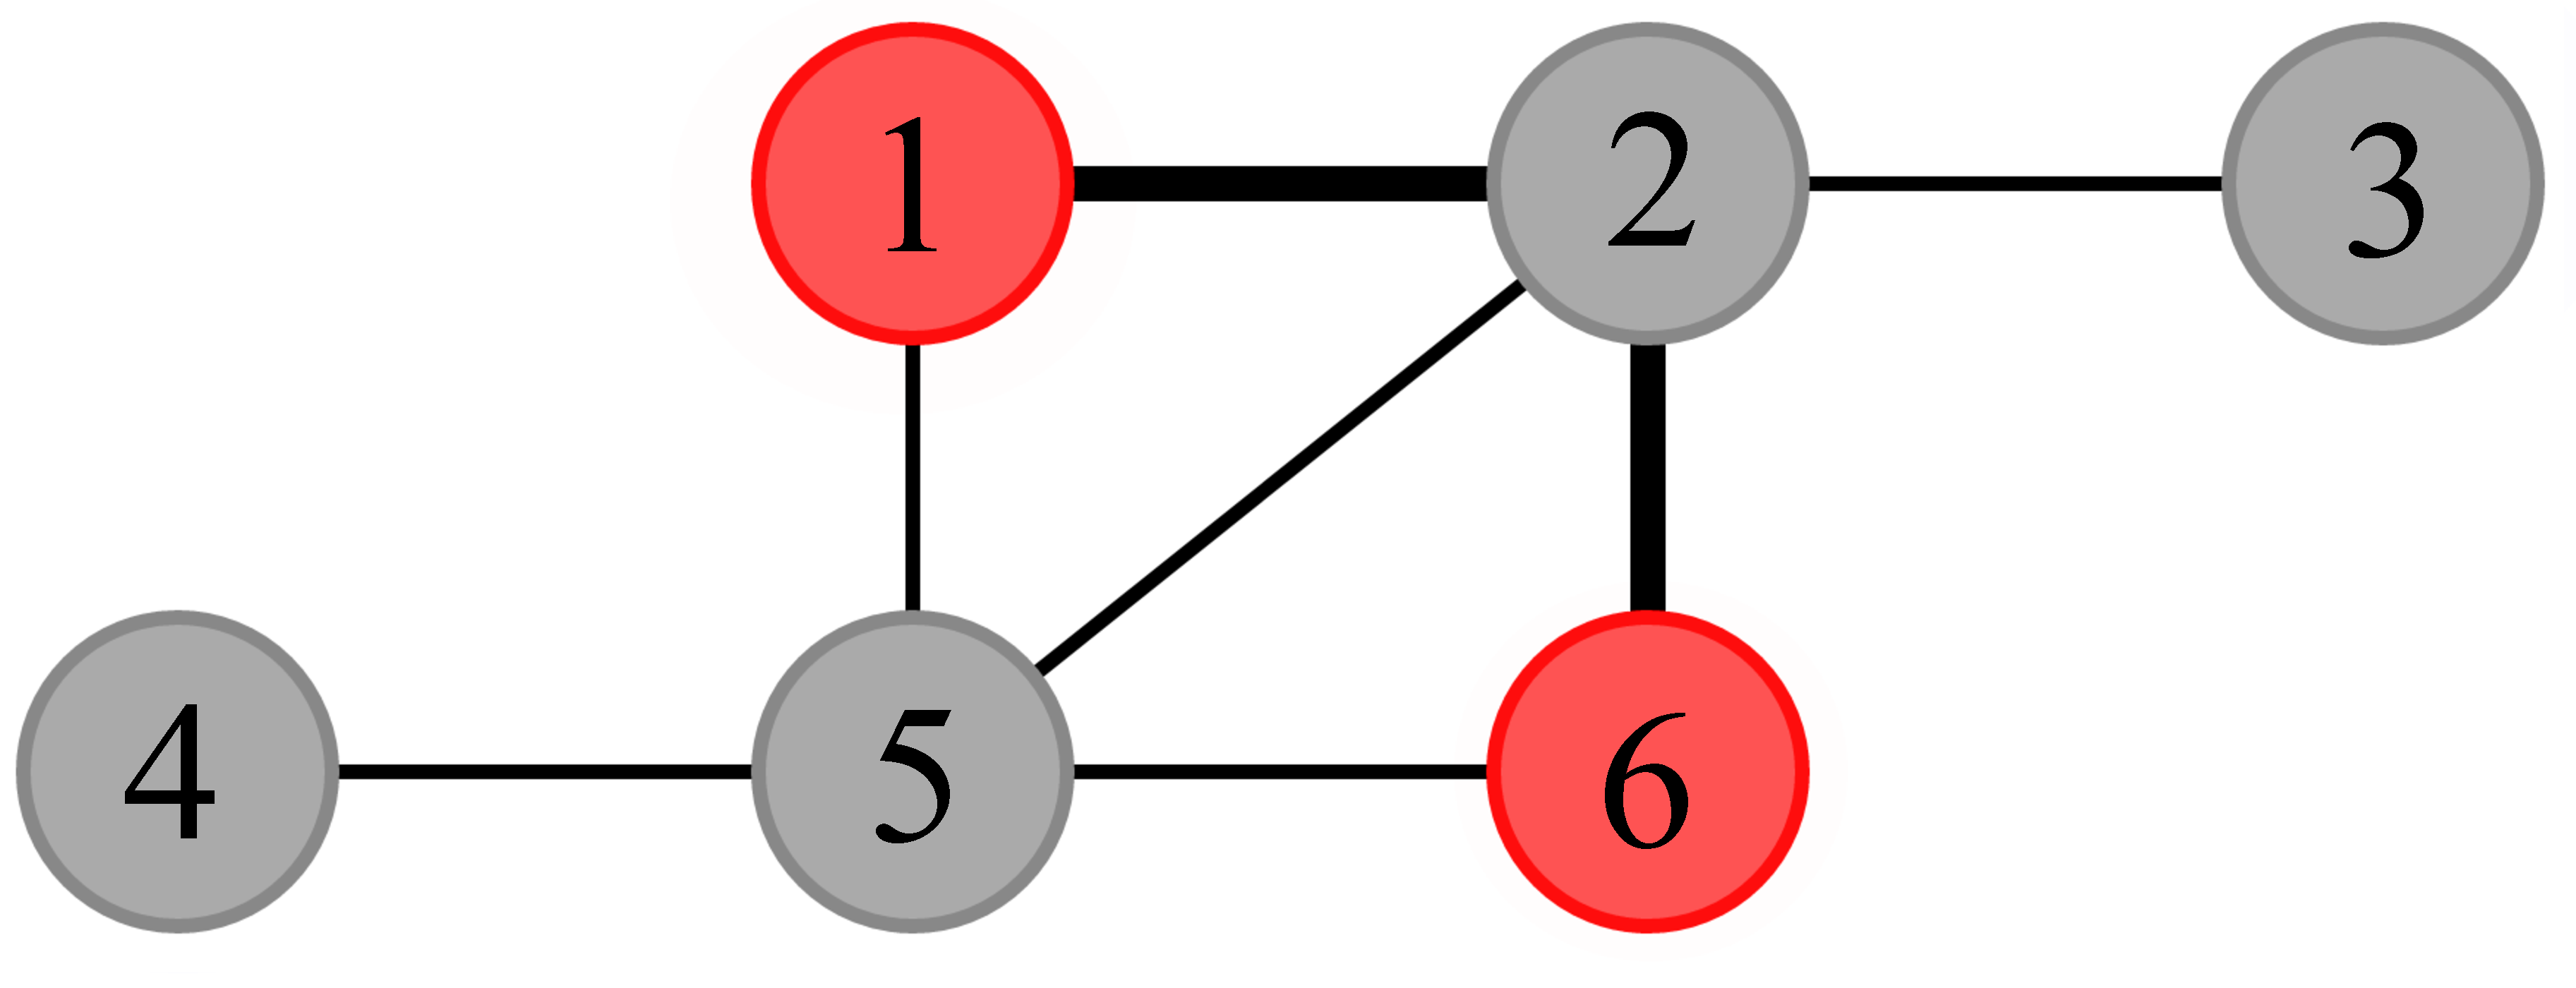
\includegraphics[width=8cm]{../figures/example-dist-1.pdf}
      \end{textblock*}
    }

    \only<8,10> {
      \begin{textblock*}{\examplewidth}(0cm,\exampleheight) % {block width} (coords)
        \centering
        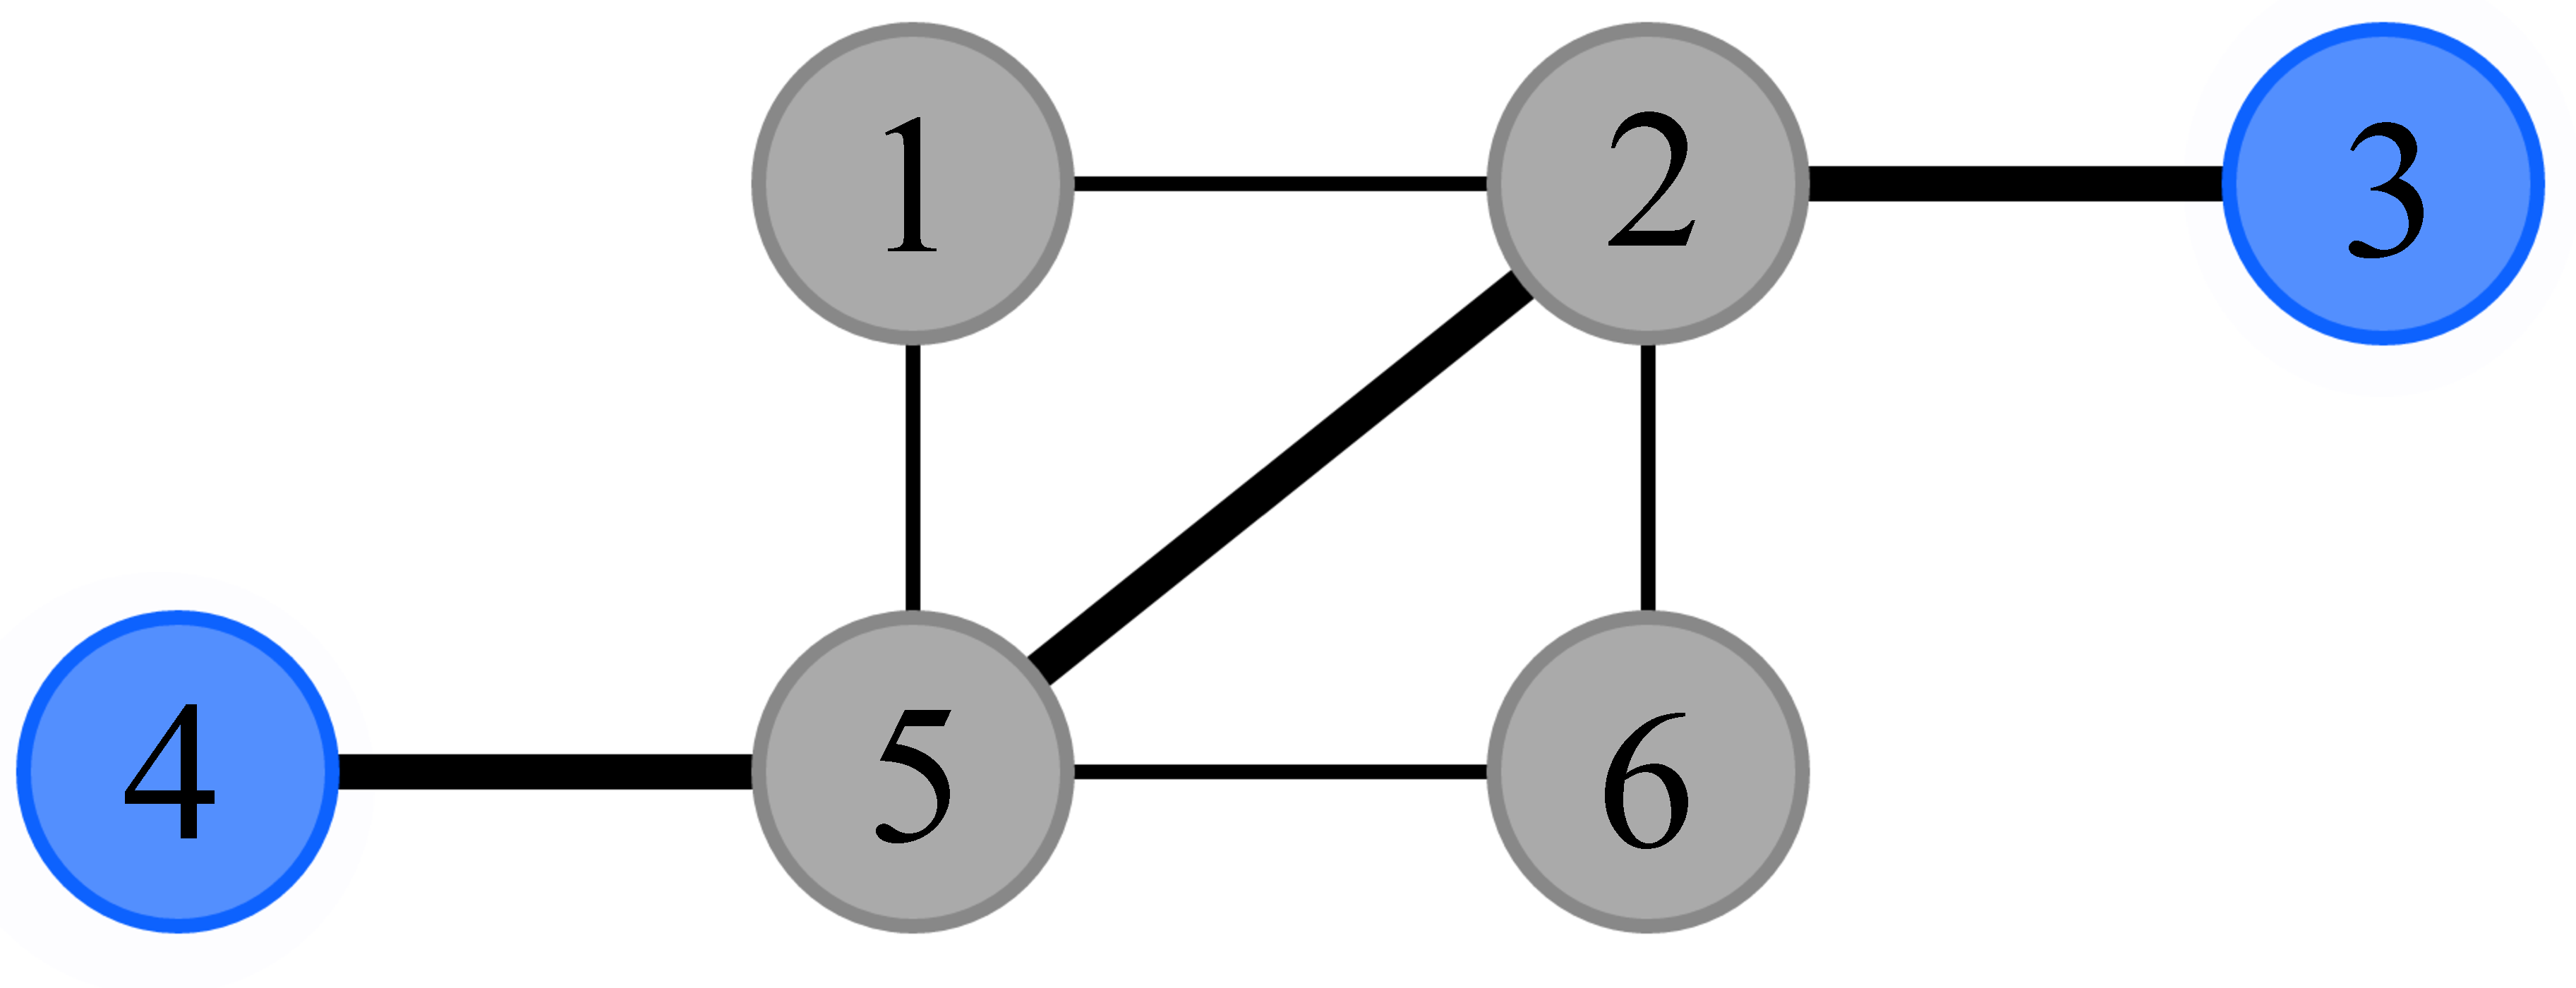
\includegraphics[width=8cm]{../figures/example-dist-2.pdf}
      \end{textblock*}
    }

    \only<12> {
      \begin{textblock*}{\examplewidth}(0cm,\exampleheight) % {block width} (coords)
        \centering
        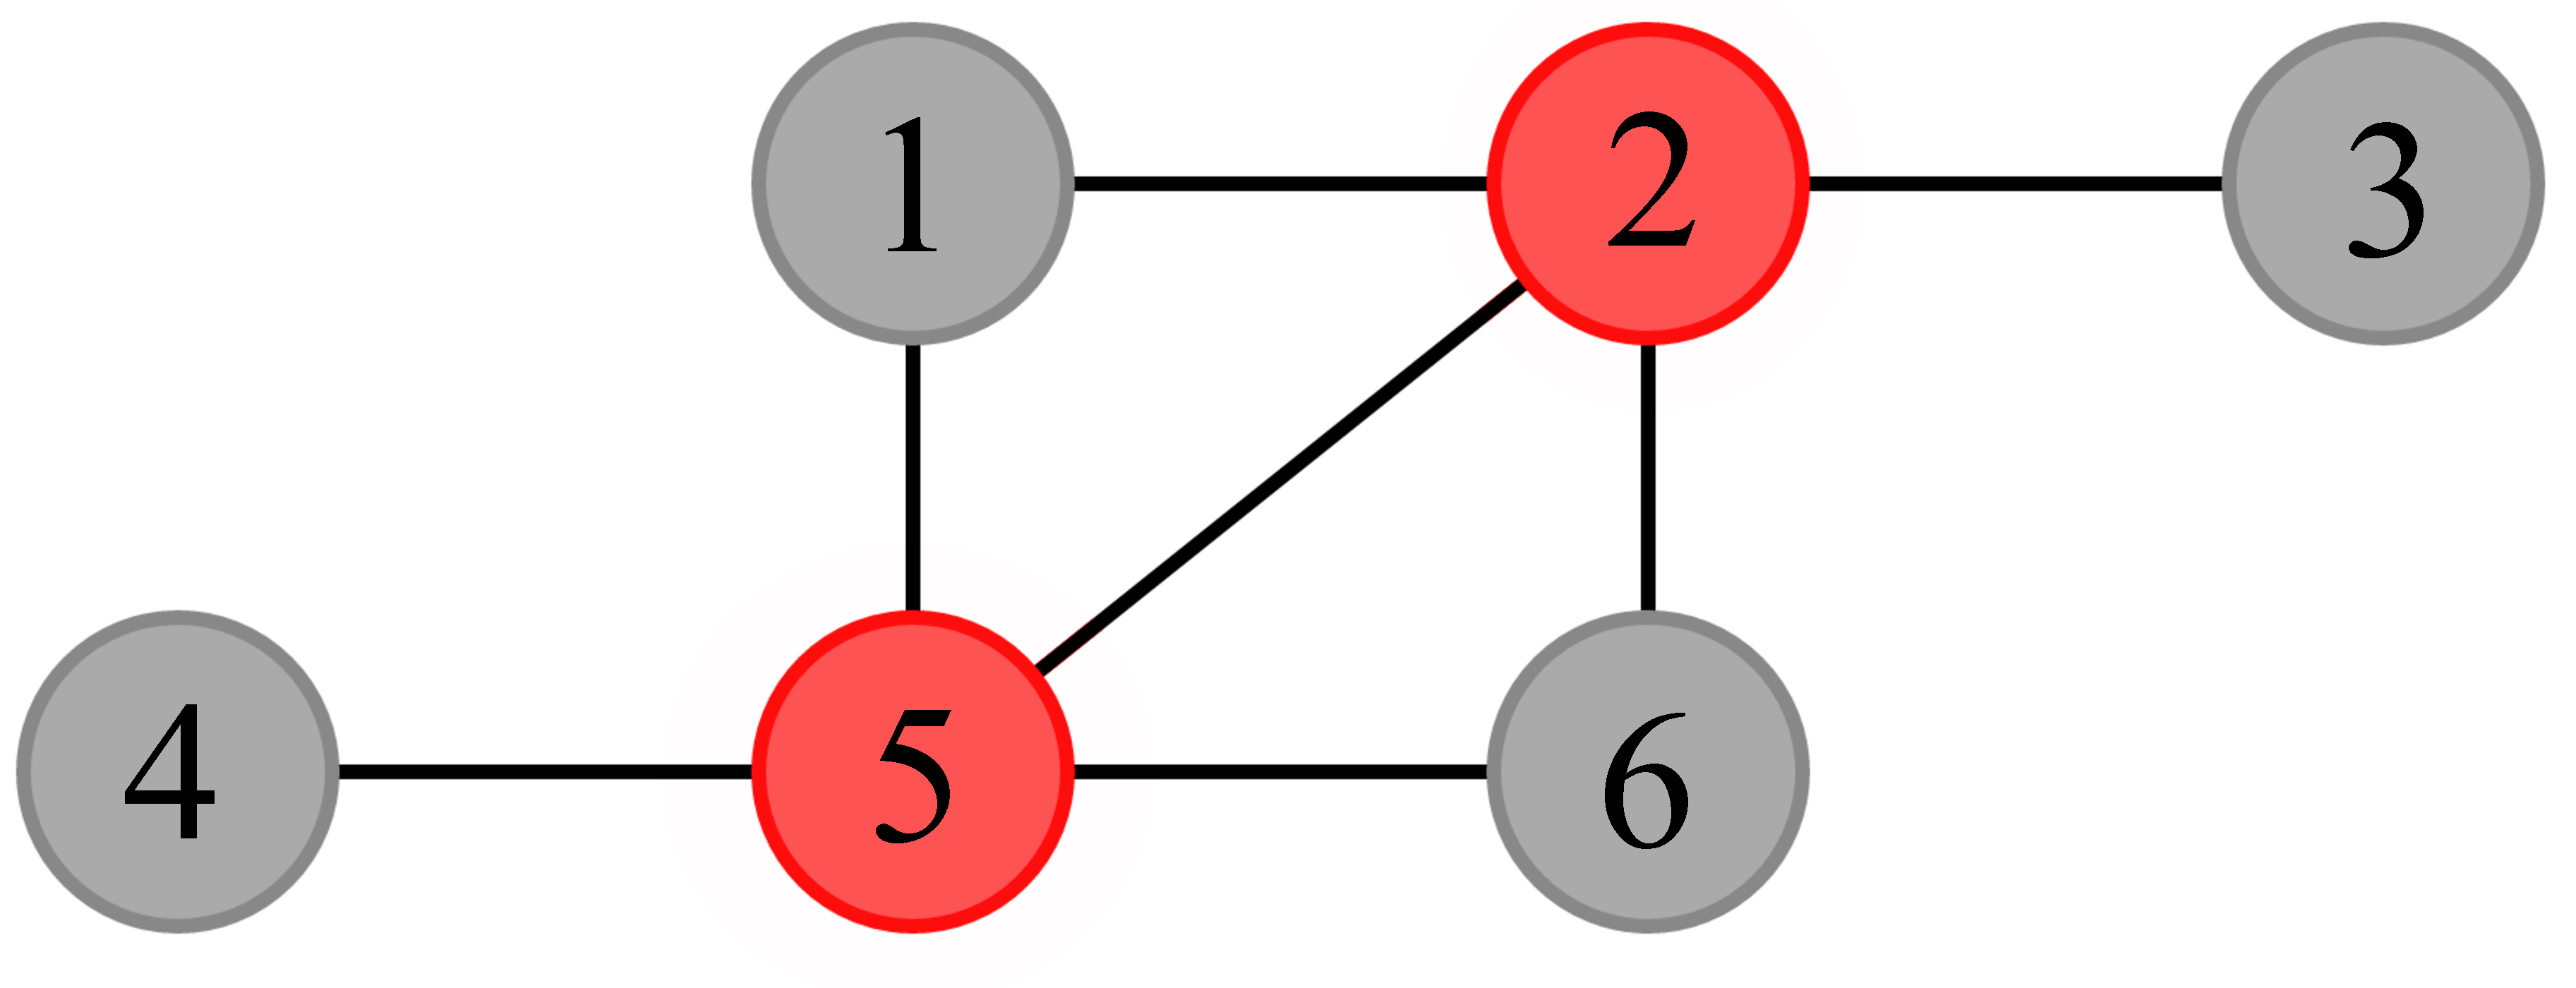
\includegraphics[width=8cm]{../figures/example-dom-1.pdf}
      \end{textblock*}
    }

    \only<13> {
      \begin{textblock*}{\examplewidth}(0cm,\exampleheight) % {block width} (coords)
        \centering
        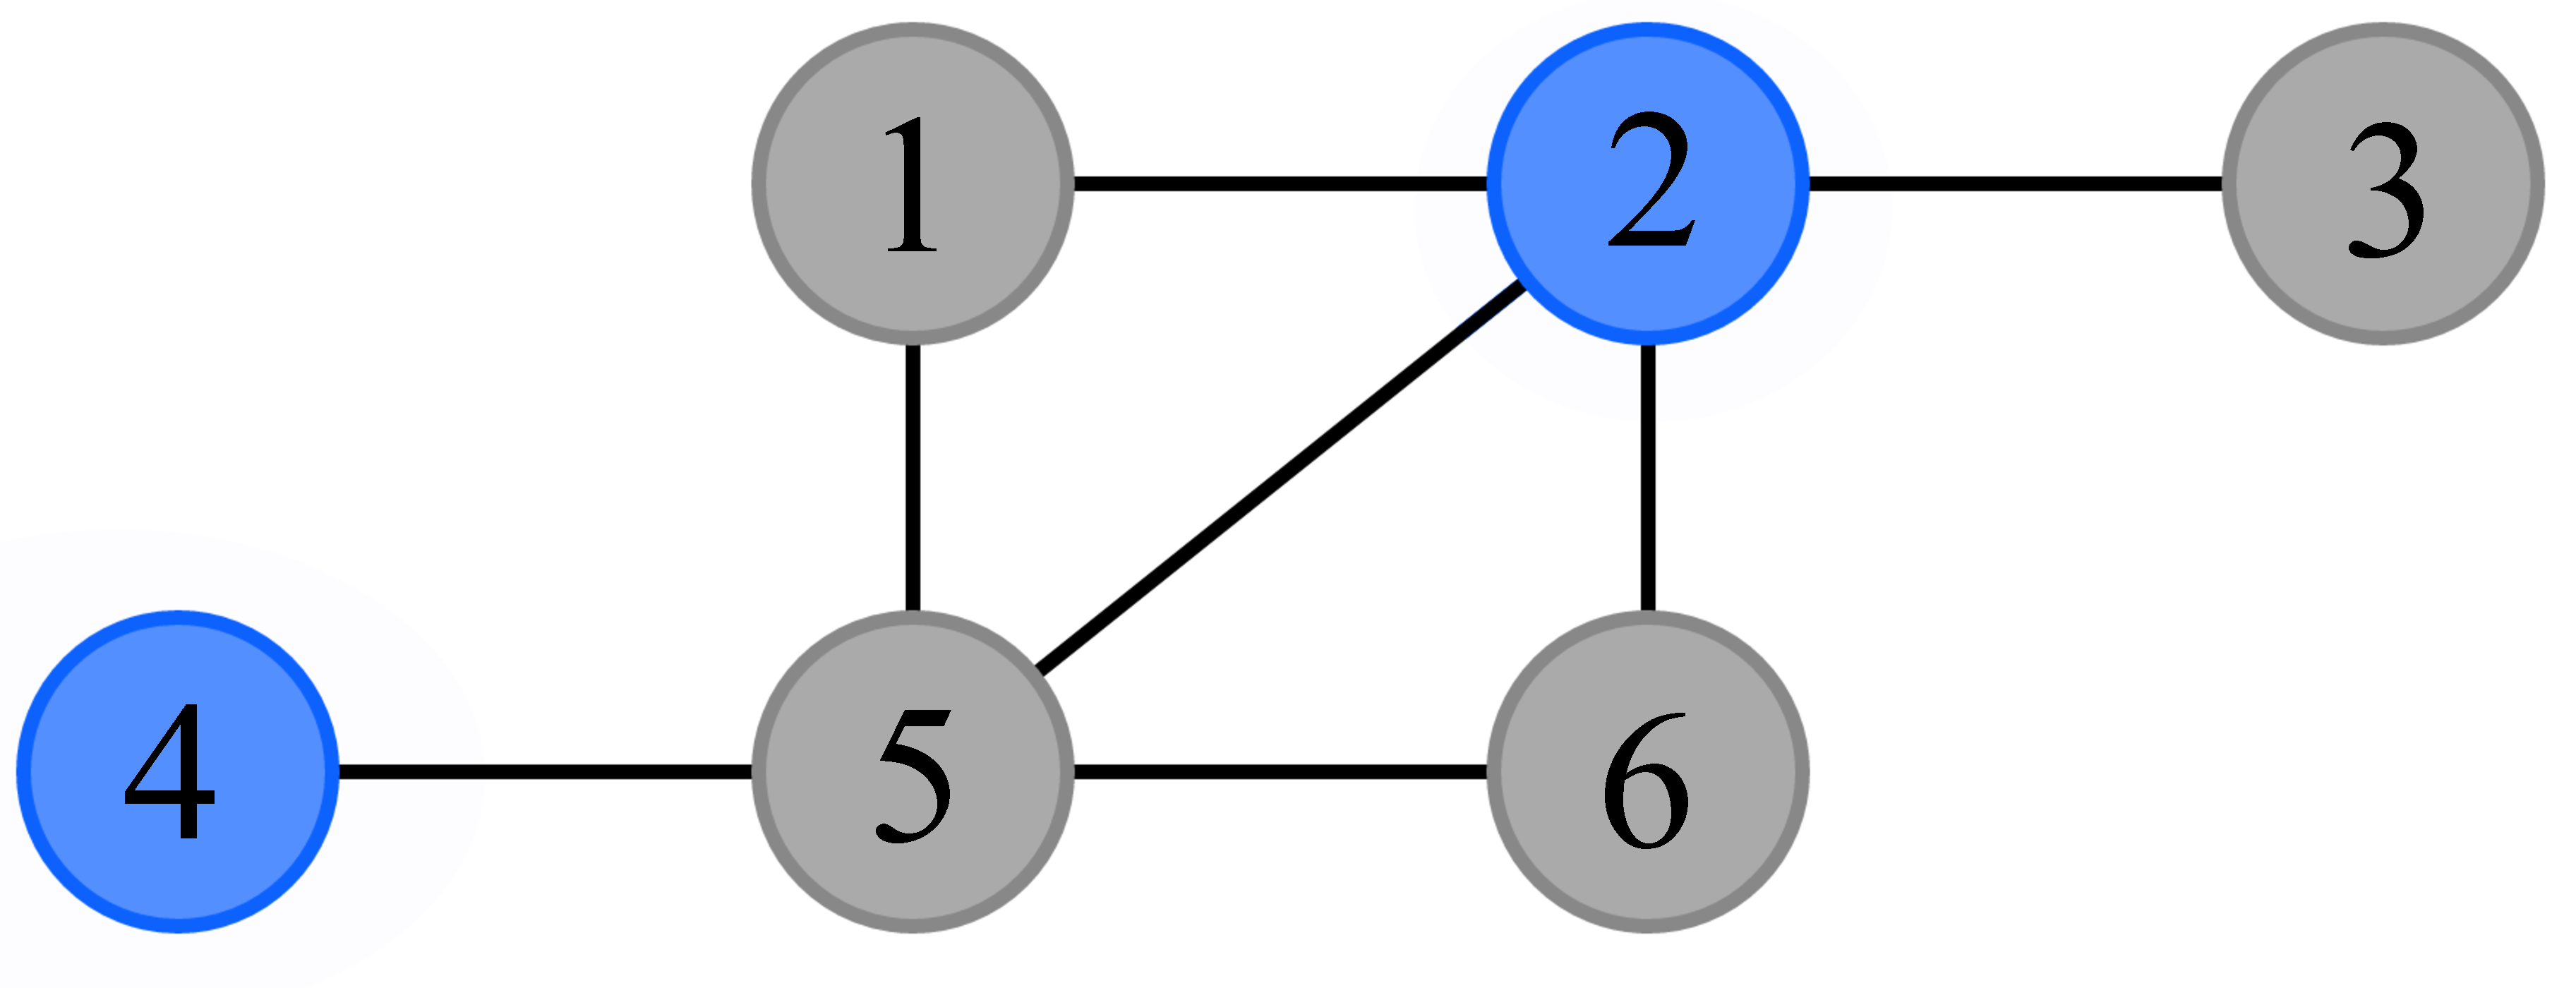
\includegraphics[width=8cm]{../figures/example-dom-2.pdf}
      \end{textblock*}
    }

    \vspace{3.5cm}

    \vfill

    \only<1-2>{
      \begin{itemize}
        \item<1-2> \textbf{Simple graph}: undirected graph with no loops.
        \pause
        \vfill
        \item \textbf{Planar graph}: no edges overlap.
      \end{itemize}
    }

    \only<3-5>{
      \begin{itemize}
        \item<3-5> \textbf{Neighborhood} of a vertex $v$: a set of all vertices adjacent to $v$ plus $v$.
        \vfill
        \only<3>{\item<4> Example: The neighborhood of vertex 1: $\{1, 2, 5\}$.}
        \only<4>{\item<4> Example: The neighborhood of vertex 1: $\{1, 2, 5\}$.}
        \only<5>{\item<5> Example: The neighborhood of vertex 5: $\{1, 2, 4, 5, 6\}$.}
      \end{itemize}
    }

    \only<6-8>{
      \begin{itemize}
        \item \textbf{Distance}: smallest number of edges to get from one vertex to another.
        \vfill
        \only<6>{\item<7> Example: distance from vertex 1 to 3: \textbf{2}.}
        \only<7>{\item<7> Example: distance from vertex 1 to 6: \textbf{2}.}
        \only<8>{\item<8> Example: distance from vertex 3 to 4: \textbf{3}.}
      \end{itemize}
    }

    \only<9-10>{
      \begin{itemize}
        \item \textbf{Distance-3-set}: contains all vertices with exactly distance 3 from each other.
        \vfill
        \only<9>{\item<7> Example: Distance from vertex 1 to 3: \textbf{2}.}
        \only<10>{\item<10> Example: The only possible distance-3-set: $\{3, 4\}$.}
      \end{itemize}
    }

    \only<11-13>{
    \vspace{0.55cm}
      \begin{itemize}
        \item \textbf{Dominating set}: a subset of vertices $D$ of $V$ such that every vertex \emph{not} in $D$ is adjacent to at least one vertex in $D$.
        \vfill
        \only<11>{\item<7> Example: The neighborhood of vertex 1: $\{1, 2, 5\}$.}
        \only<12>{\item<12> Example: $\{2, 5\}$}
        \only<13>{\item<13> Example: $\{2, 4\}$}
      \end{itemize}
    }


  \end{frame}

  \subsection{Vertex Coloring}

  \begin{frame}
    \frametitle{Vertex Coloring}

    \begin{textblock*}{\examplewidth}(0cm,\exampleheight) % {block width} (coords)
      \centering
      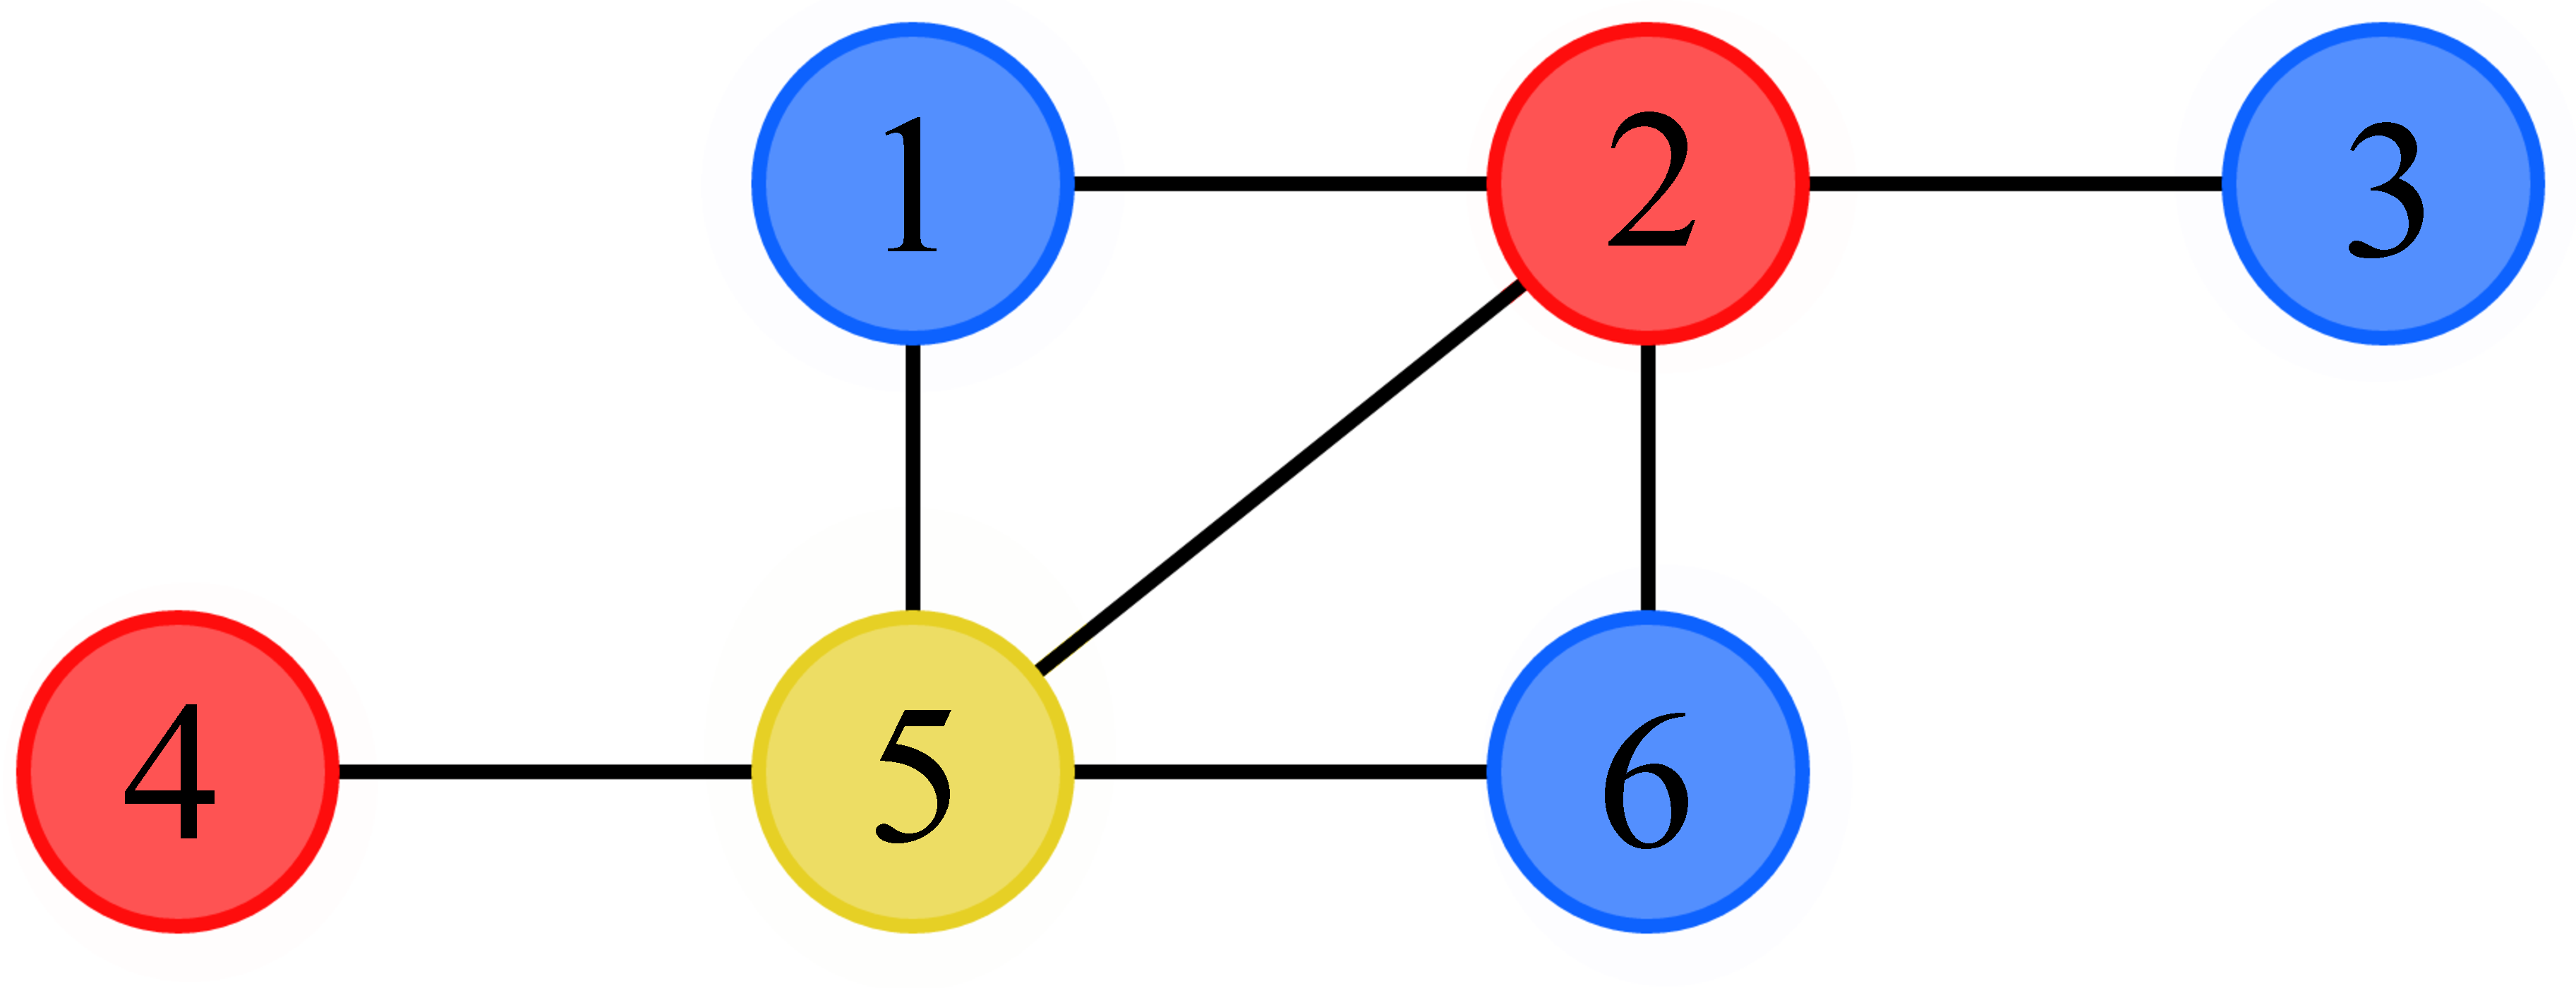
\includegraphics[width=8cm]{../figures/example-vcp.pdf}
    \end{textblock*}

    \vspace{4.5cm}
    \vfill

    \begin{itemize}
      \item A \textbf{proper vertex coloring} of a graph $G$ assigns colors to \emph{every} vertex such that no two adjacent vertices share the same color.
      \pause
      \vfill
      \item The \textbf{chromatic number} of $G$ is the minimum number of colors needed to properly color $G$.
    \end{itemize}
  \end{frame}

  \begin{frame}
    \frametitle{Conflict-Free Coloring}

    \begin{textblock*}{\examplewidth}(0cm,\exampleheight) % {block width} (coords)
      \centering
      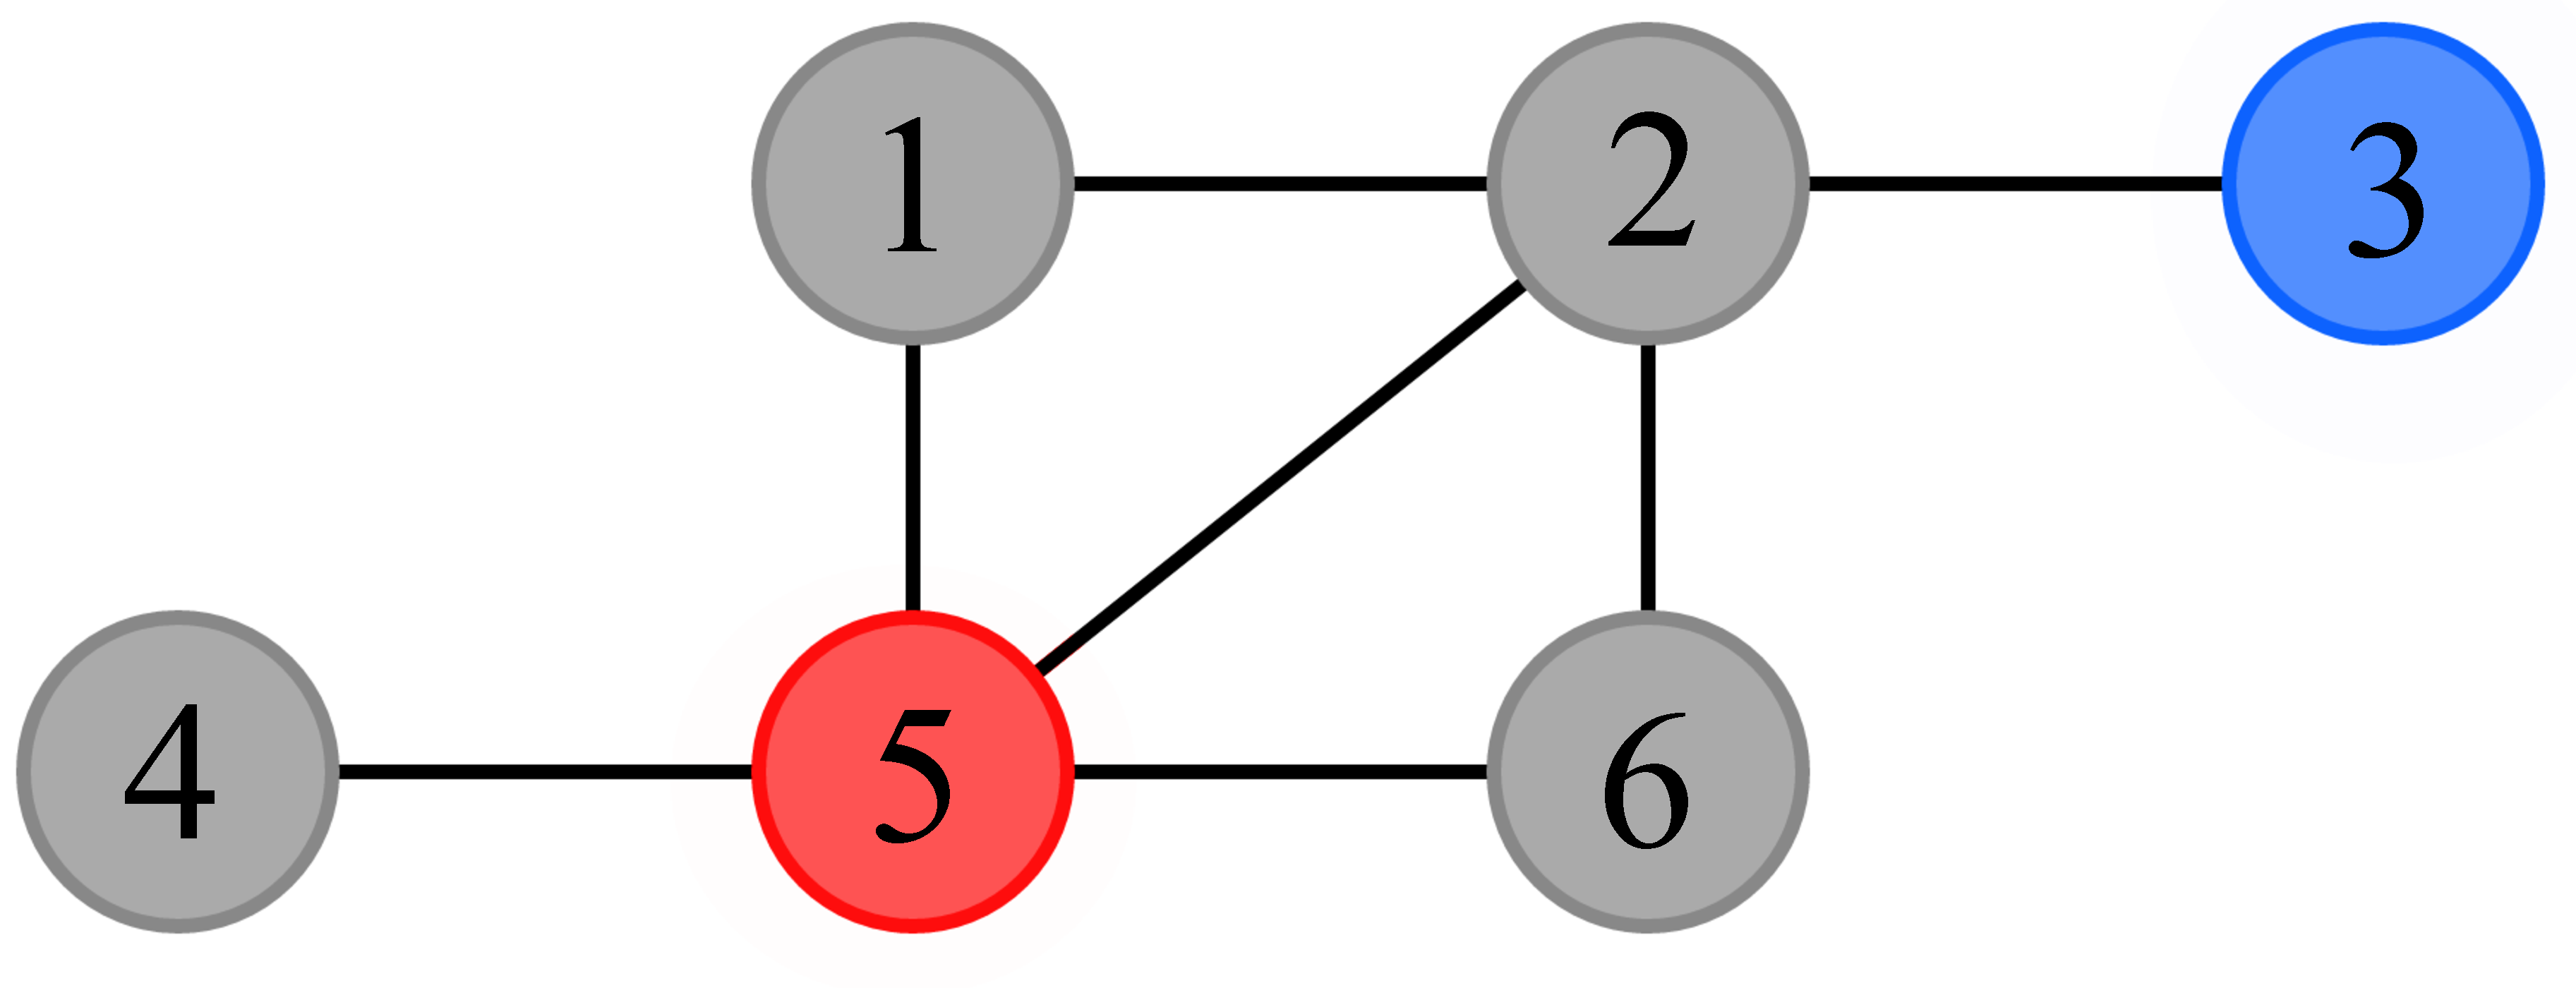
\includegraphics[width=8cm]{../figures/example-cfcp.pdf}
    \end{textblock*}

    \vspace{4.5cm}
    \vfill

    \begin{itemize}
      \item<1-2> A \textbf{conflict-free coloring} of a graph $G$ assigns colors to \emph{some} vertices such that the neighborhood of every vertex contains at least one unique color.
      \vfill
      \pause
      \item<2> Proper vertex colorings are also conflict-free colorings.
    \end{itemize}
  \end{frame}

  \begin{frame}
    \frametitle{Conflict-Free Coloring}

    \begin{textblock*}{\examplewidth/2}(0cm,\exampleheight) % {block width} (coords)
      \centering
      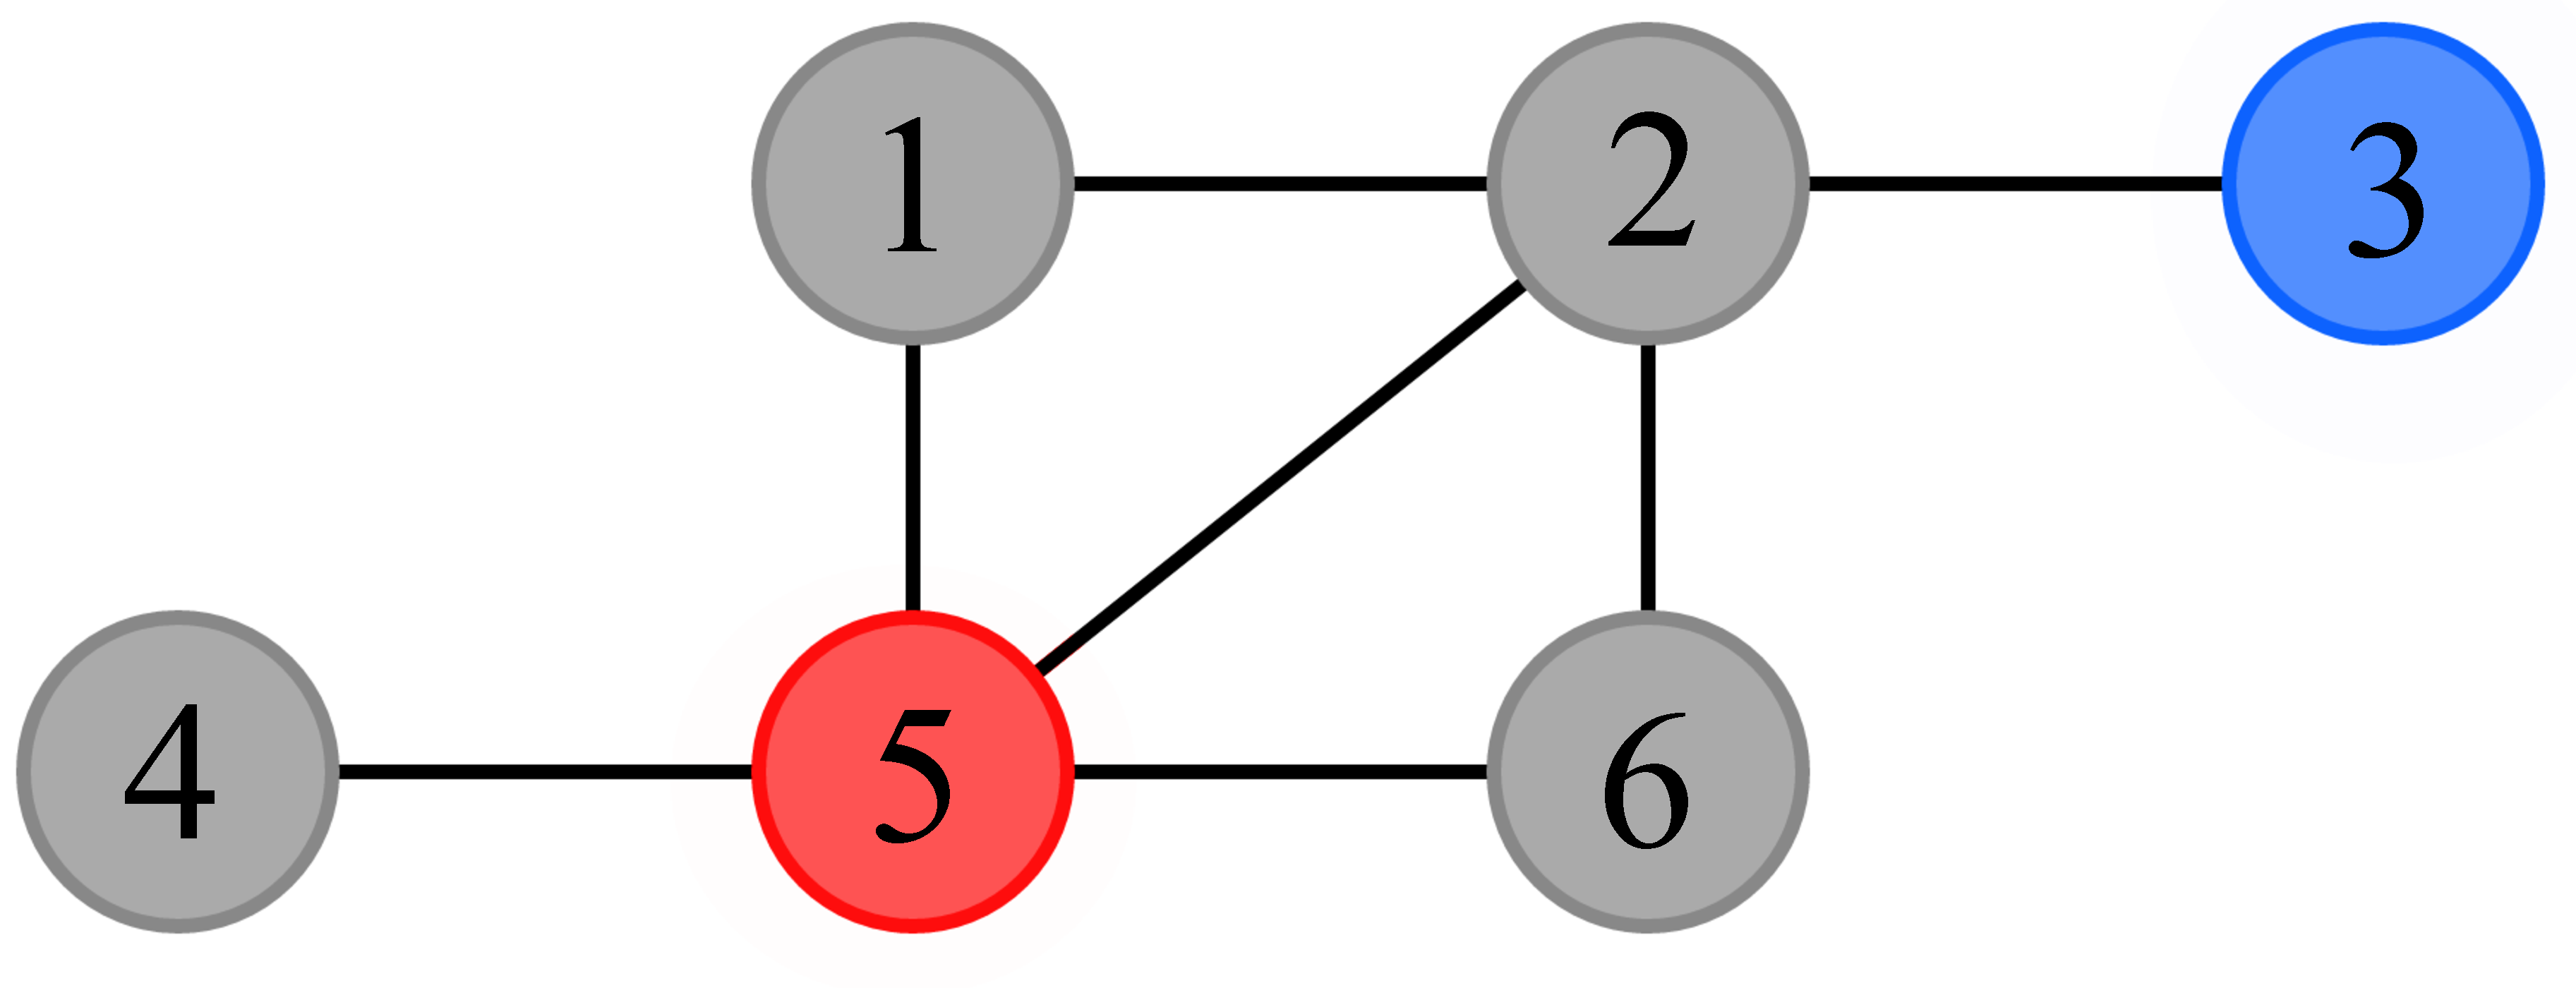
\includegraphics[width=6.5cm]{../figures/example-cfcp.pdf}
    \end{textblock*}

    \begin{textblock*}{\examplewidth/2}(8cm,\exampleheight) % {block width} (coords)
      \centering
      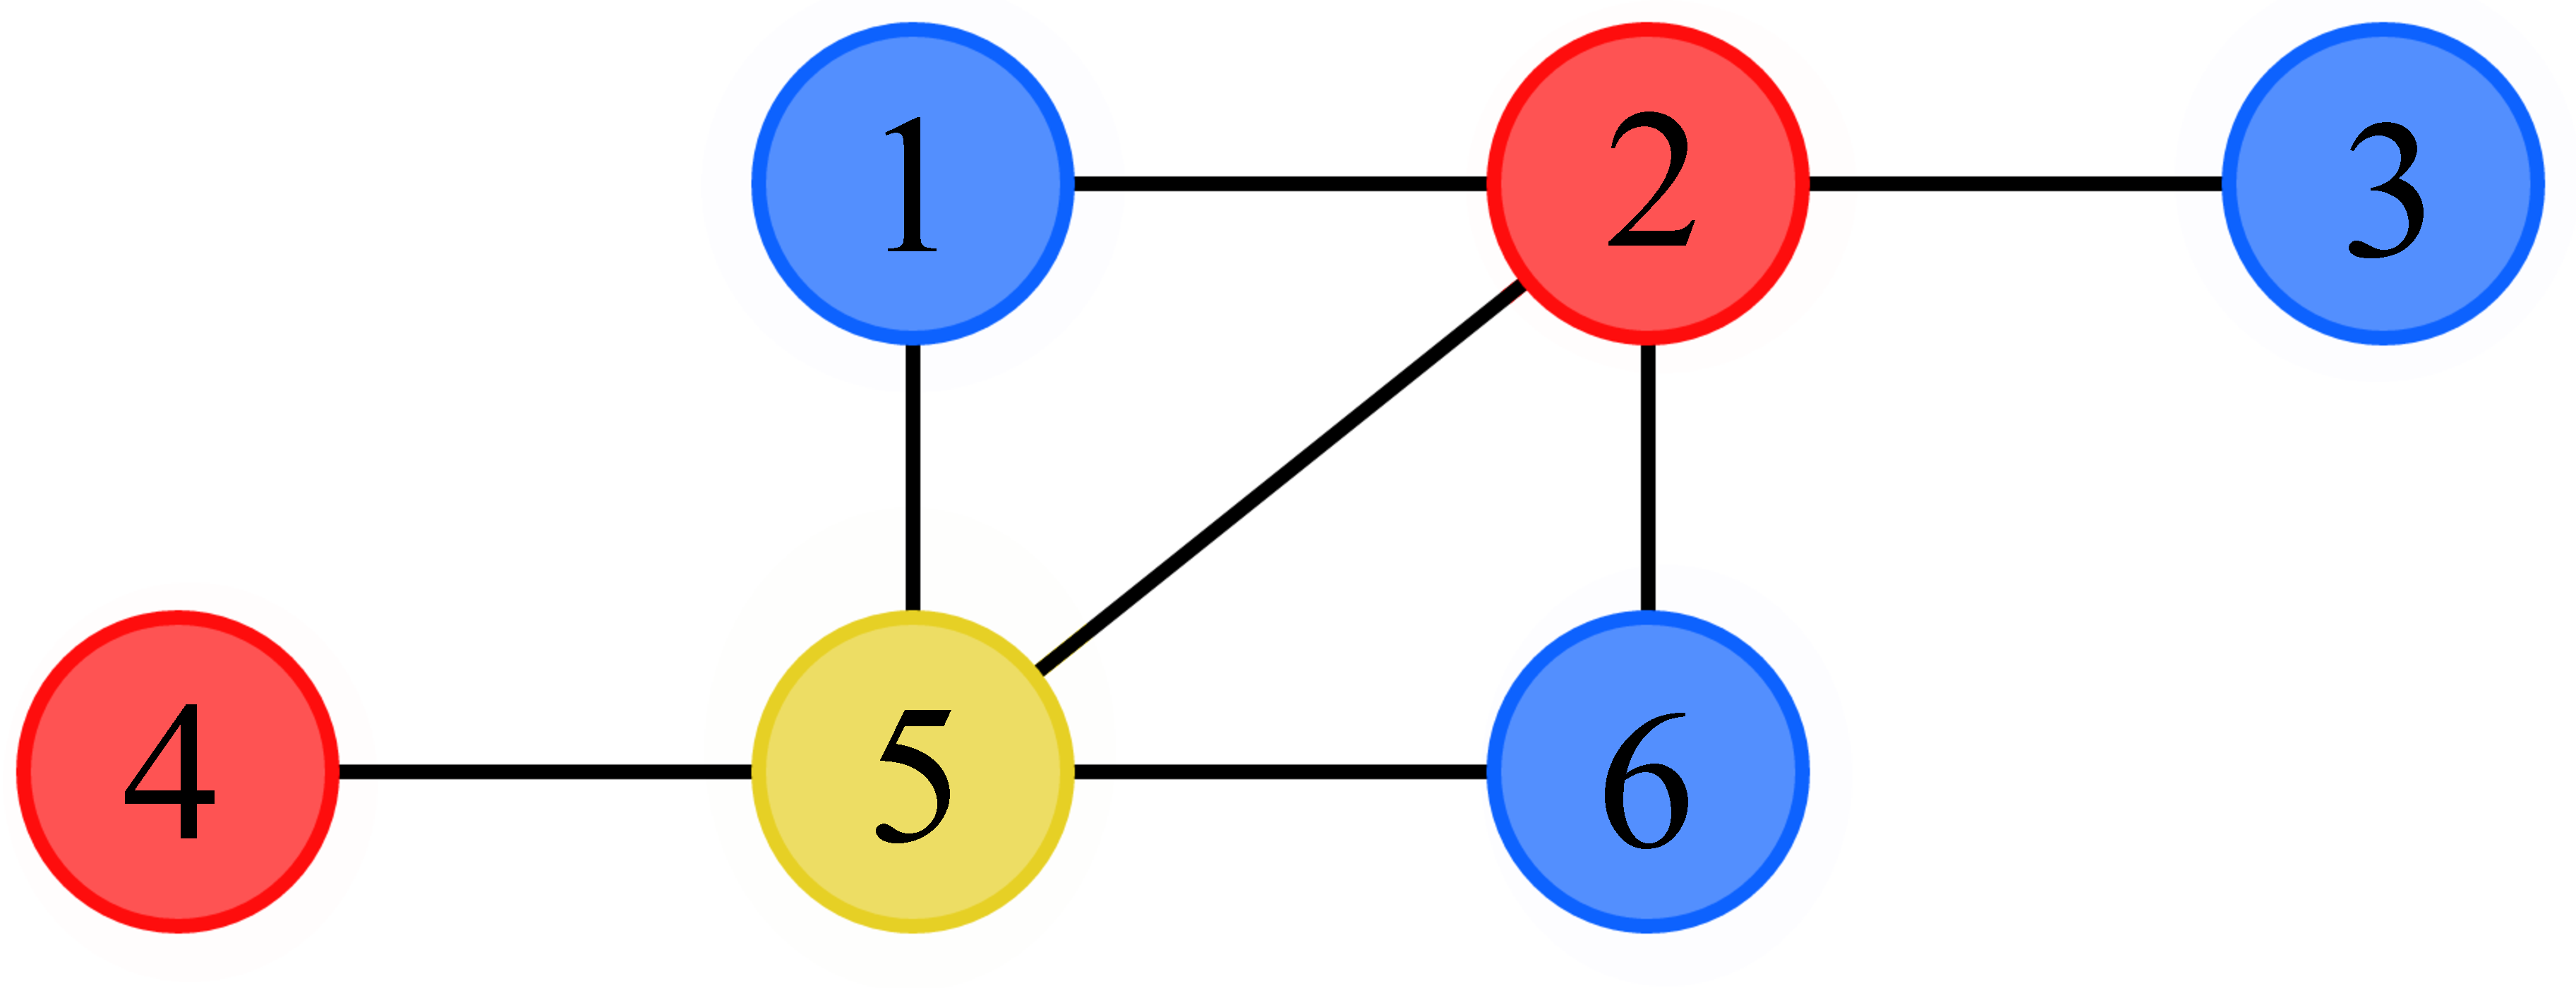
\includegraphics[width=6.5cm]{../figures/example-vcp.pdf}
    \end{textblock*}

    \vspace{3cm}

    \begin{center}
      Every vertex $v$ has at least one unique color within its neighborhood.
    \end{center}

    \pause

    \begin{columns}
      \begin{column}{0.5\textwidth}
        \begin{itemize}[leftmargin=1.4cm]
          \item[$v$ = 1:] $\{1: none,\ 2: none,\ 5: \textbf{red}\}$
          \item[$v$ = 2:] $\{1: none,\ 2: none,\ 3: \textbf{blue},$ \newline $\quad 5: red,\ 6: none\}$
          \item[$v$ = 3:] $\{2: none,\ 3: \textbf{blue}\}$
        \end{itemize}
      \end{column}

      \pause

      \begin{column}{0.5\textwidth}
        \begin{itemize}[leftmargin=1.4cm]
          \item[$v$ = 1:] $\{1: \textbf{blue},\ 2: red,\ 5: yellow\}$
          \item[$v$ = 2:] $\{1: blue,\ 2: \textbf{red},\ 3: blue,$ \newline $\quad 5: yellow,\ 6: blue\}$
          \item[$v$ = 3:] $\{2: red,\ 3: \textbf{blue}\}$
        \end{itemize}
      \end{column}
    \end{columns}

  \end{frame}

  \subsection{Conflict-Free Coloring}

  \begin{frame}
    \frametitle{Conflict-Free Coloring Examples}

    \begin{textblock*}{\examplewidth}(1cm,\exampleheight) % {block width} (coords)
      Incorrect conflict-free colorings and their fixes:
    \end{textblock*}

    \vspace{0.5cm}

    \pause

    \begin{columns}
      \begin{column}{0.33333\textwidth}
        \only<2>{
          \begin{figure}[h]
            \centering
            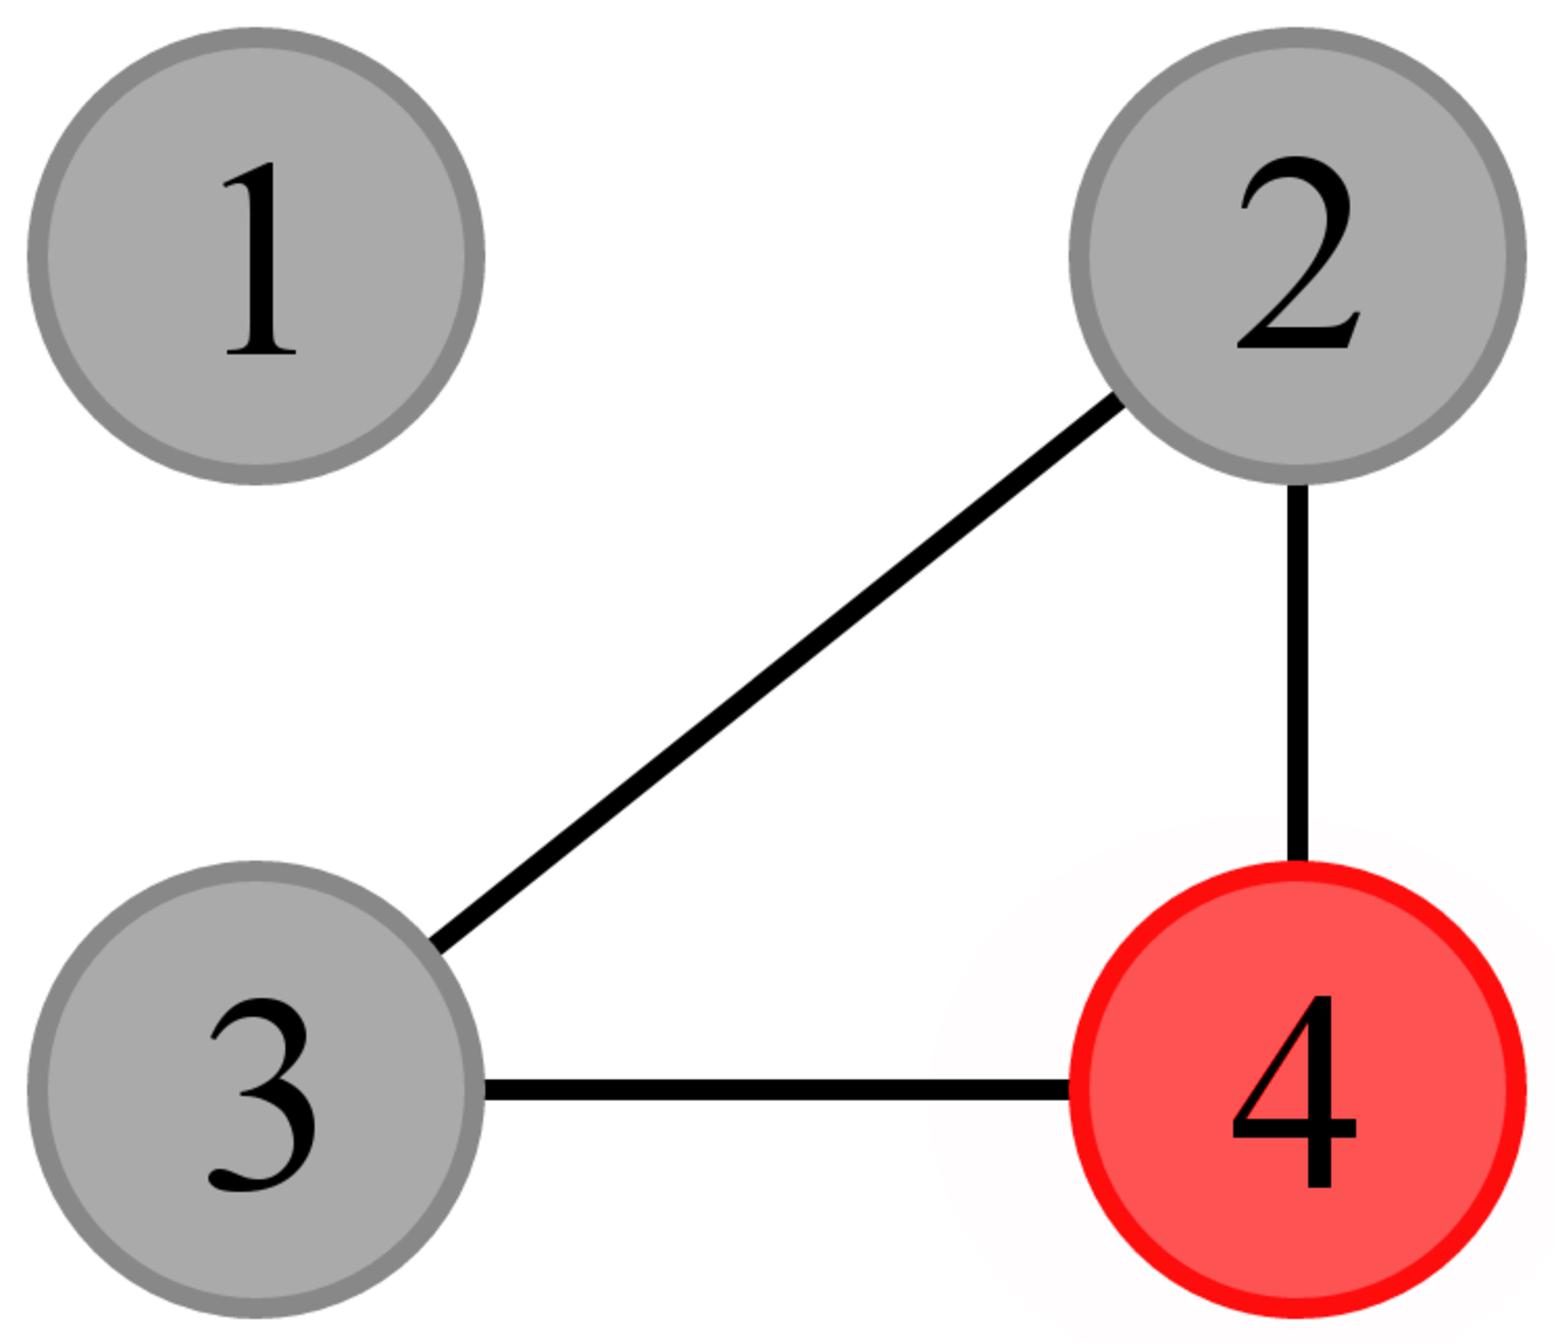
\includegraphics[width=3cm]{../figures/examples-1-incorrect-1.pdf}
          \end{figure}
        }

        \only<3-7>{
          \begin{figure}[h]
            \centering
            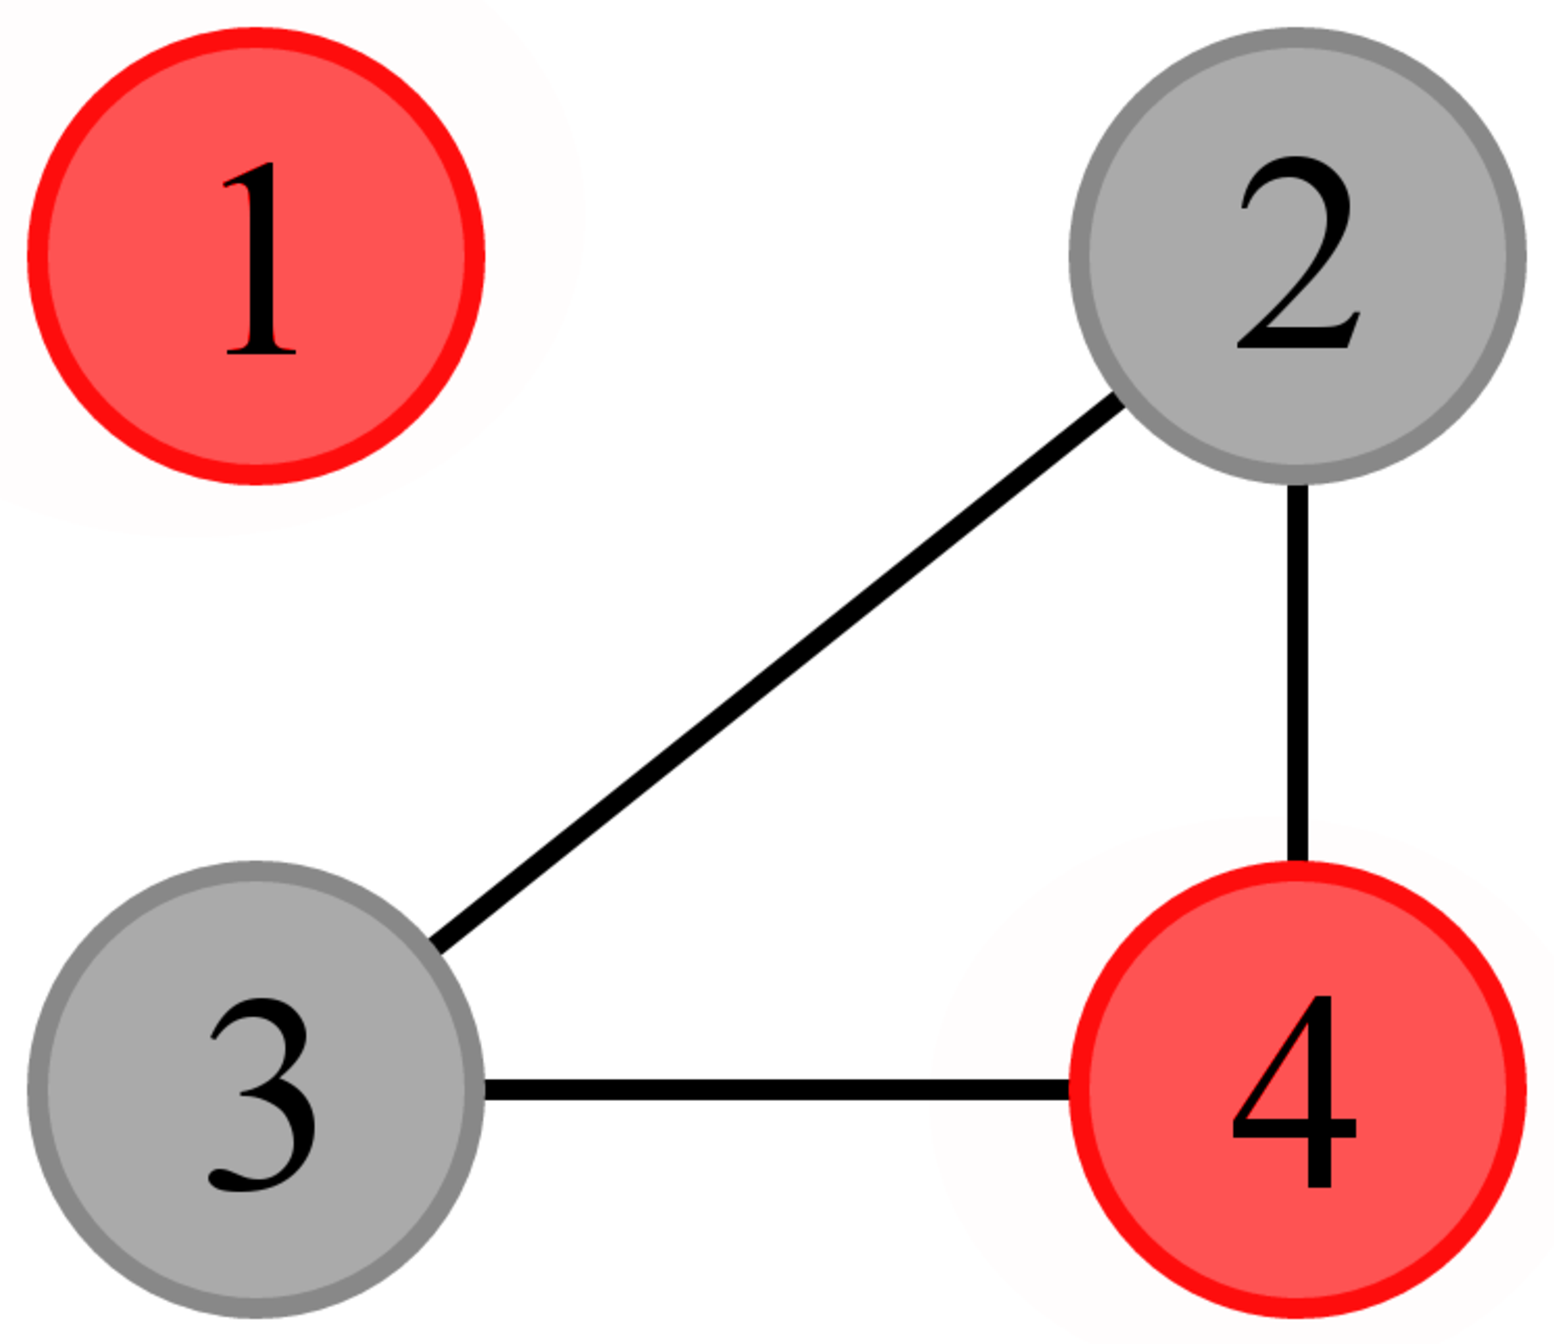
\includegraphics[width=3cm]{../figures/examples-1-incorrect-1-corrected.pdf}
          \end{figure}
        }

        \centering
        Vertex 1 does not have a unique color in its neighborhood.
      \end{column}

      \pause
      \pause

      \begin{column}{0.33333\textwidth}

        \only<4>{
        \begin{figure}[h]
          \centering
          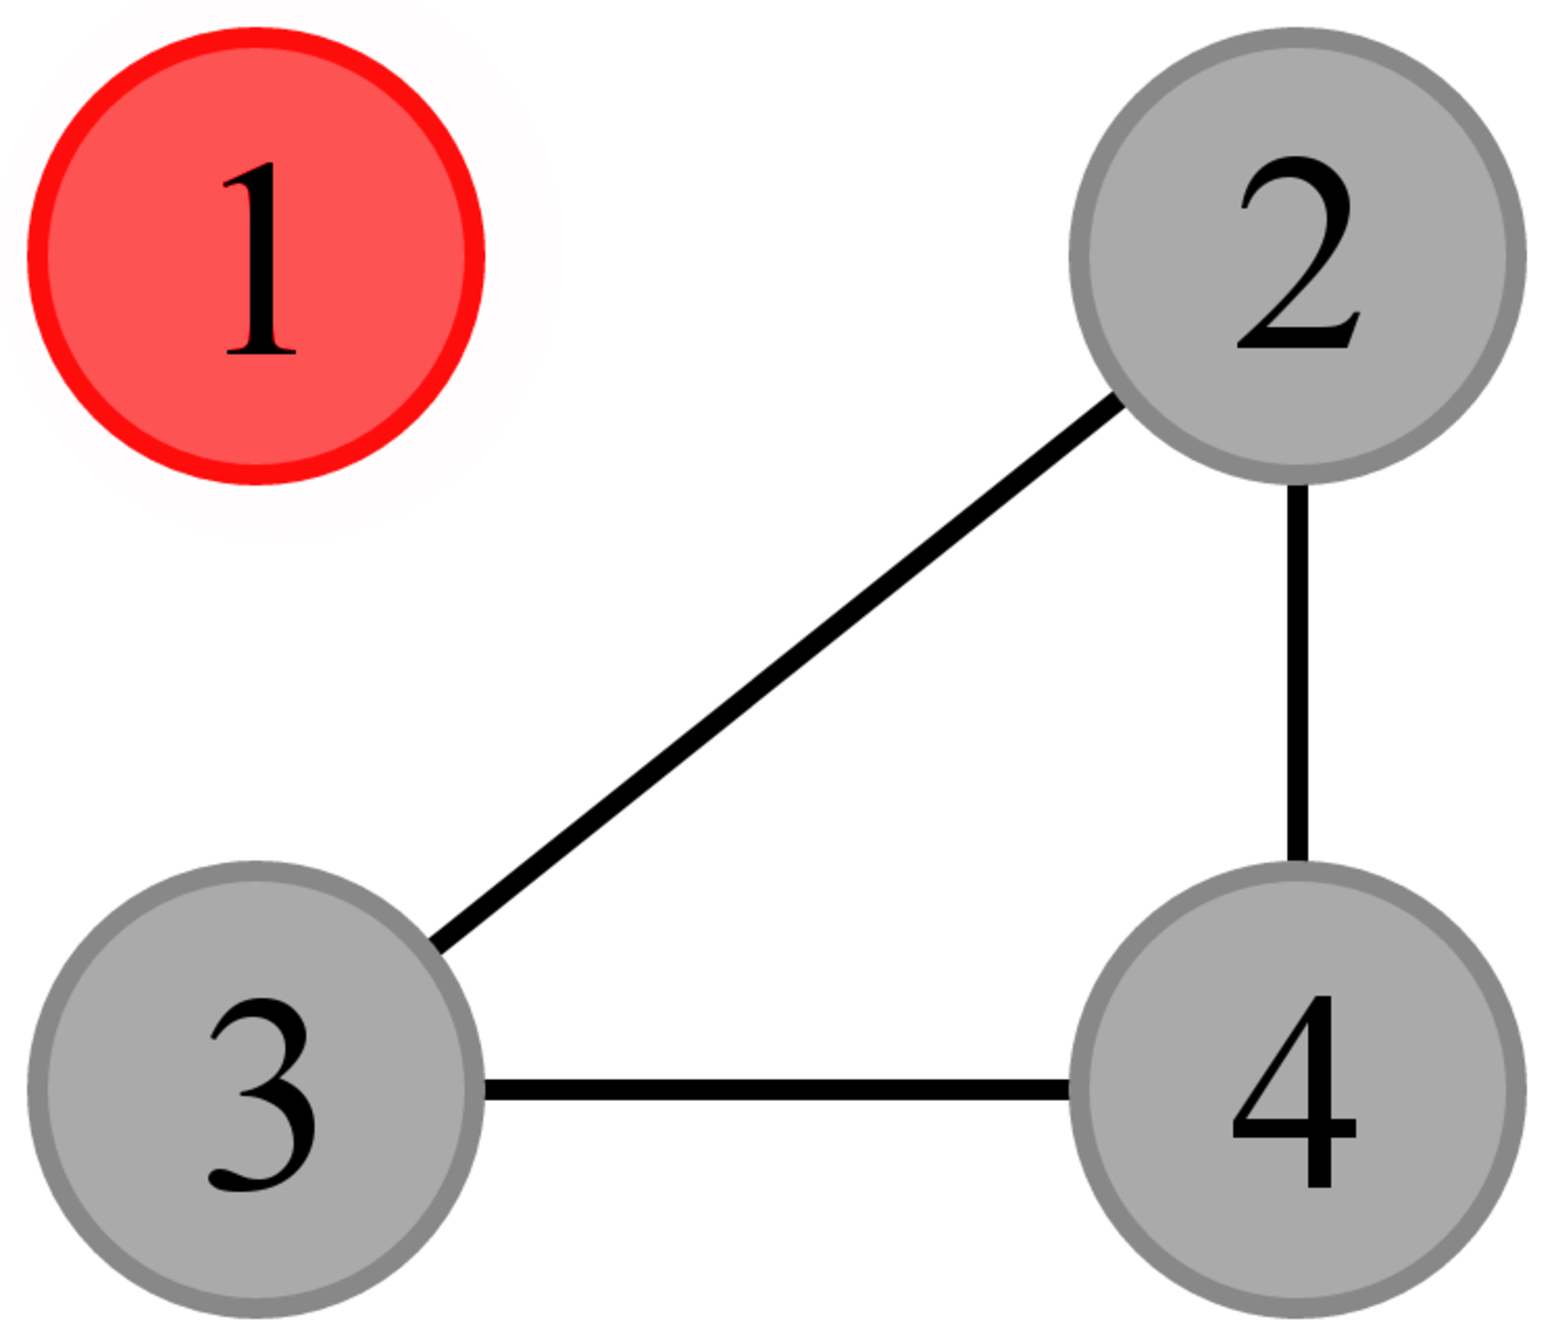
\includegraphics[width=3cm]{../figures/examples-1-incorrect-2.pdf}
        \end{figure}
        }

        \only<5-7>{
        \begin{figure}[h]
          \centering
          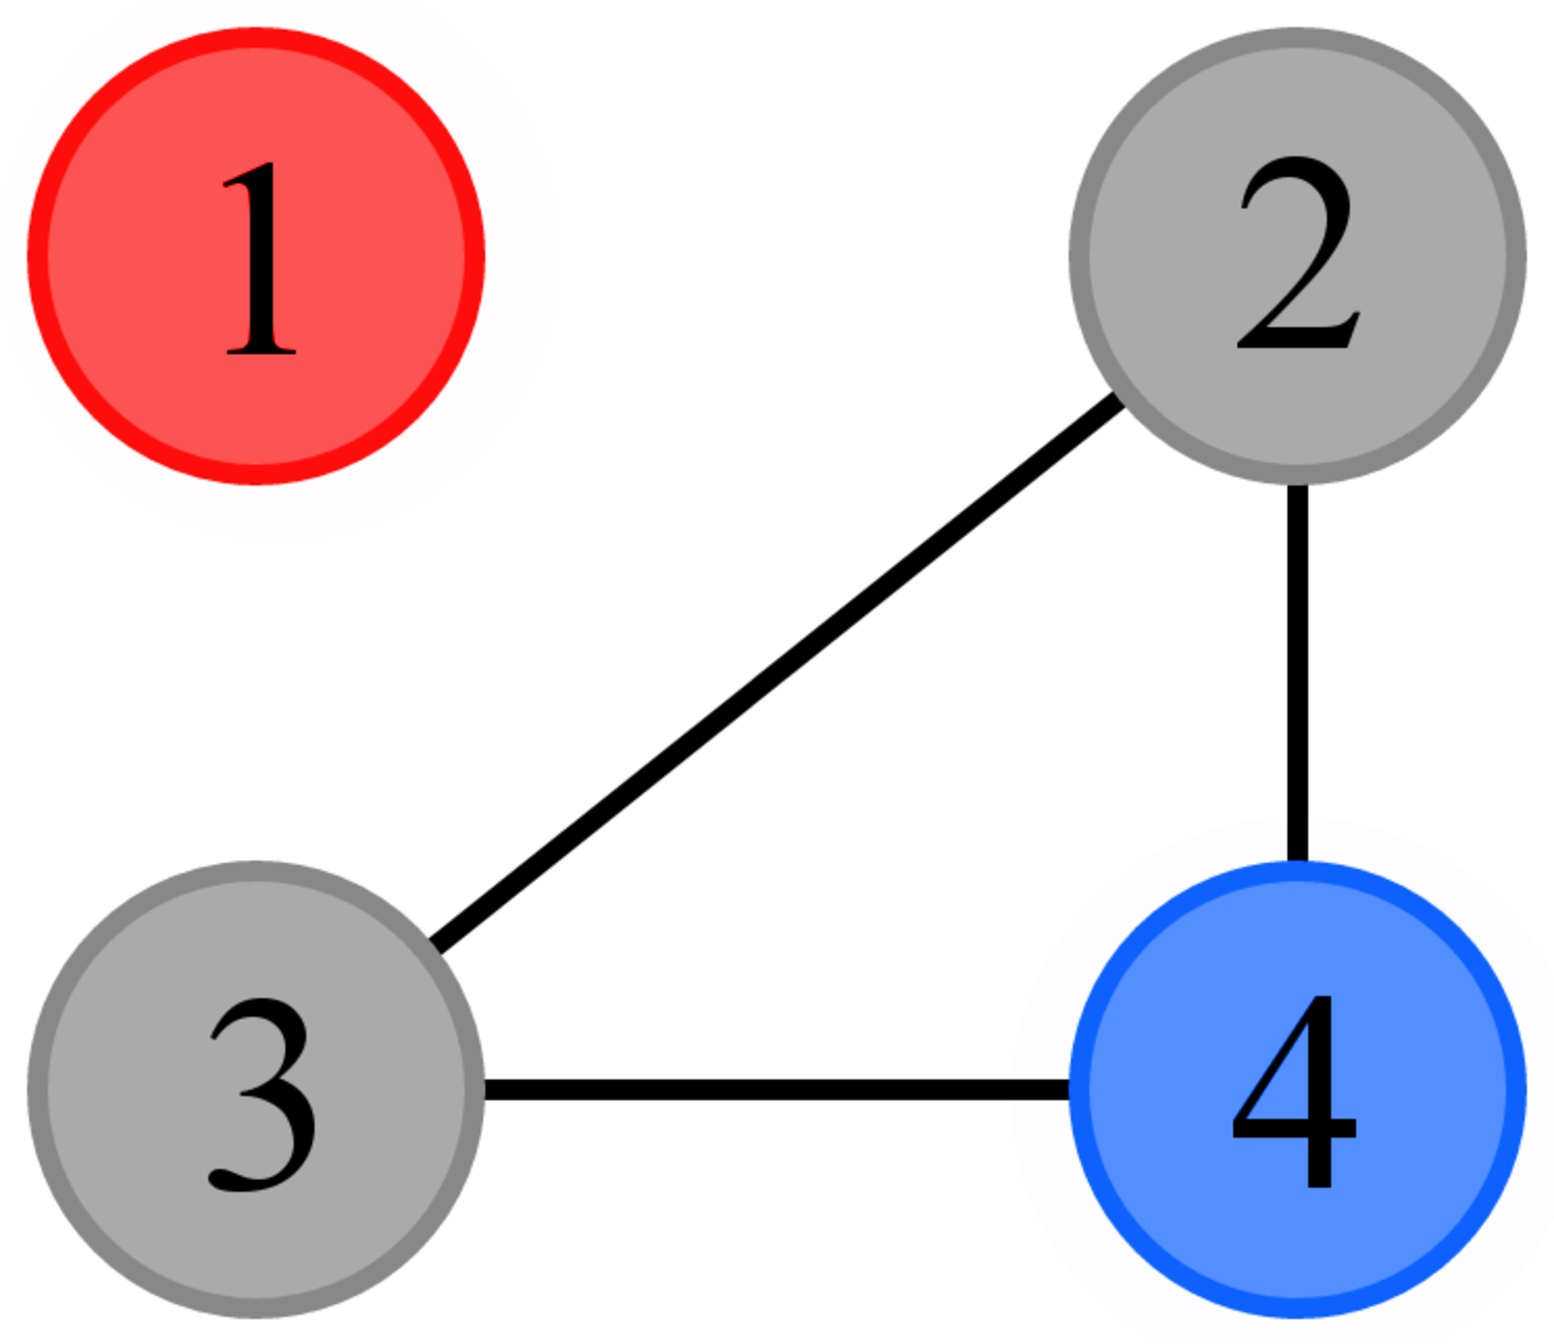
\includegraphics[width=3cm]{../figures/examples-1-incorrect-2-corrected.pdf}
        \end{figure}
        }

        \centering
        Vertices $\{2, 3, 4\}$ do not have a unique color in their neighborhoods.
      \end{column}

      \pause
      \pause

      \begin{column}{0.33333\textwidth}

        \only<6>{
        \begin{figure}[h]
          \centering
          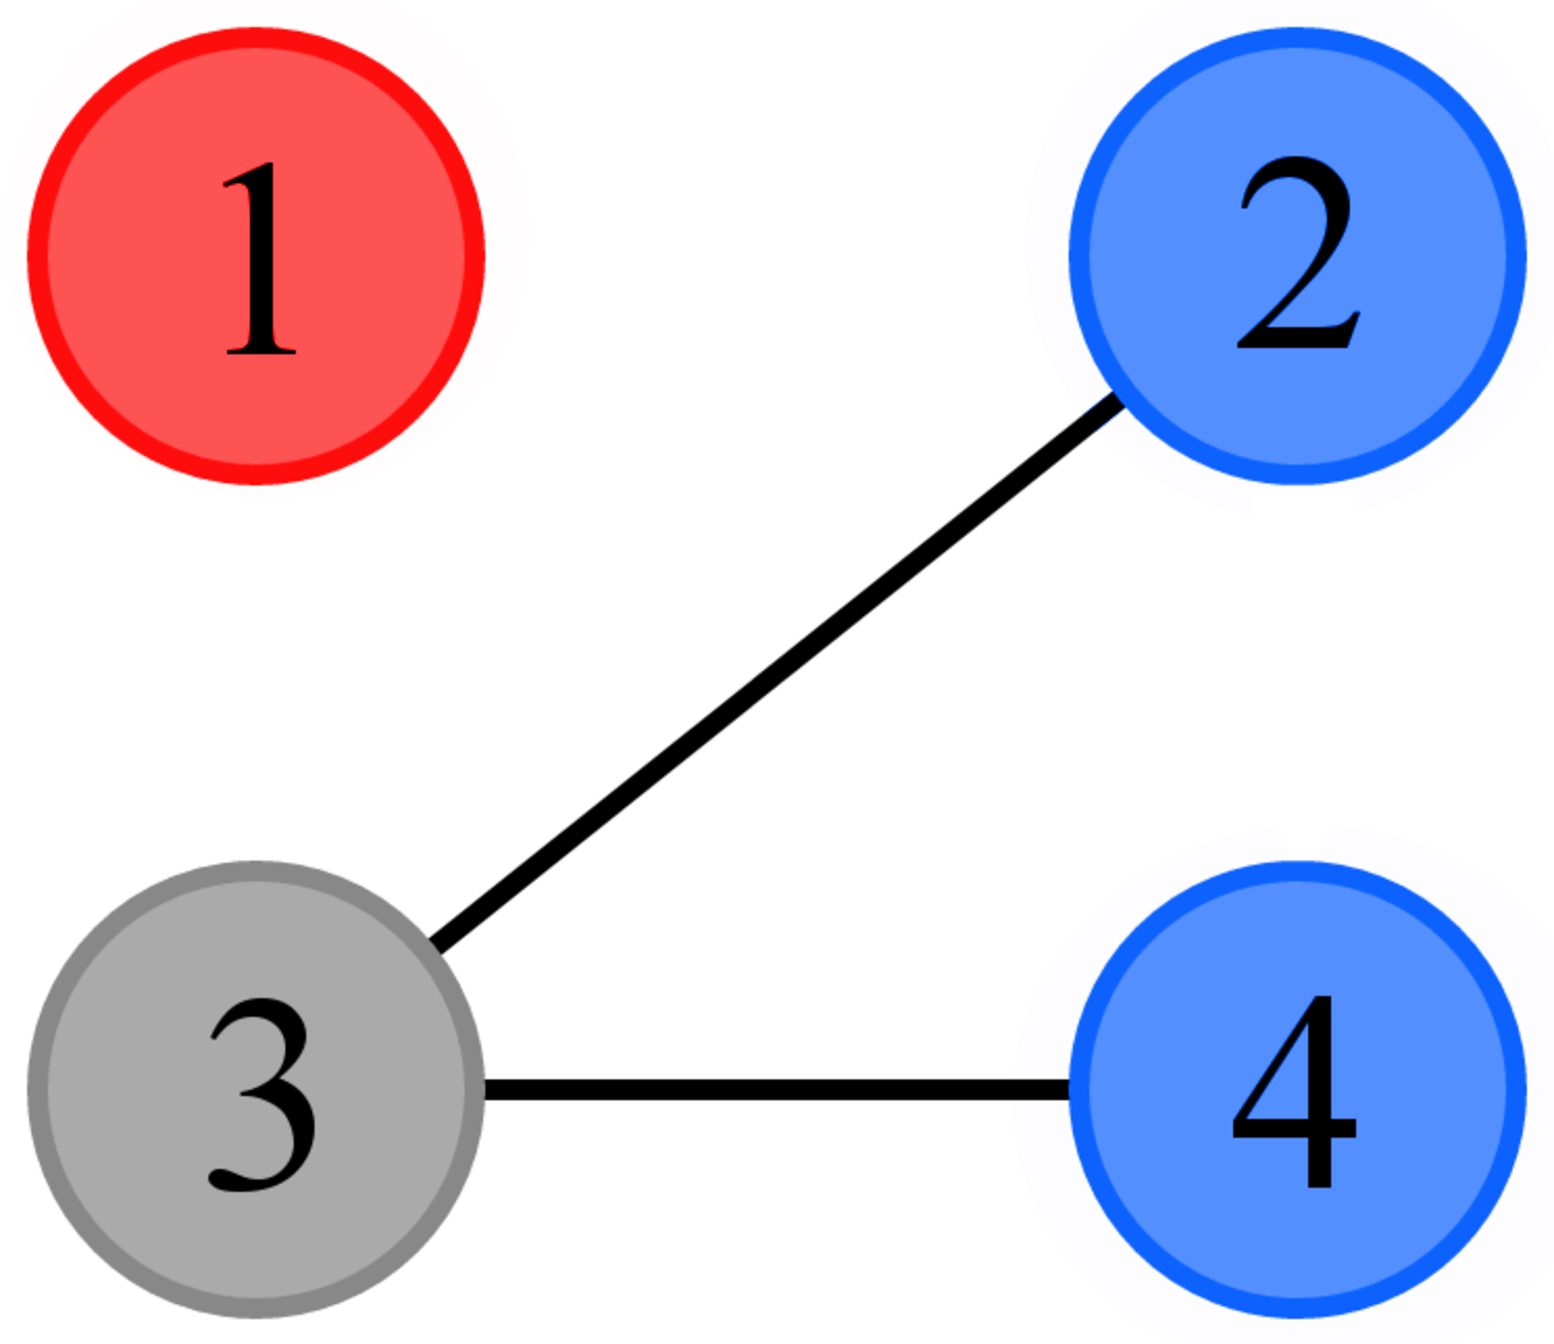
\includegraphics[width=3cm]{../figures/examples-1-incorrect-3.pdf}
        \end{figure}
        }

        \only<7>{
        \begin{figure}[h]
          \centering
          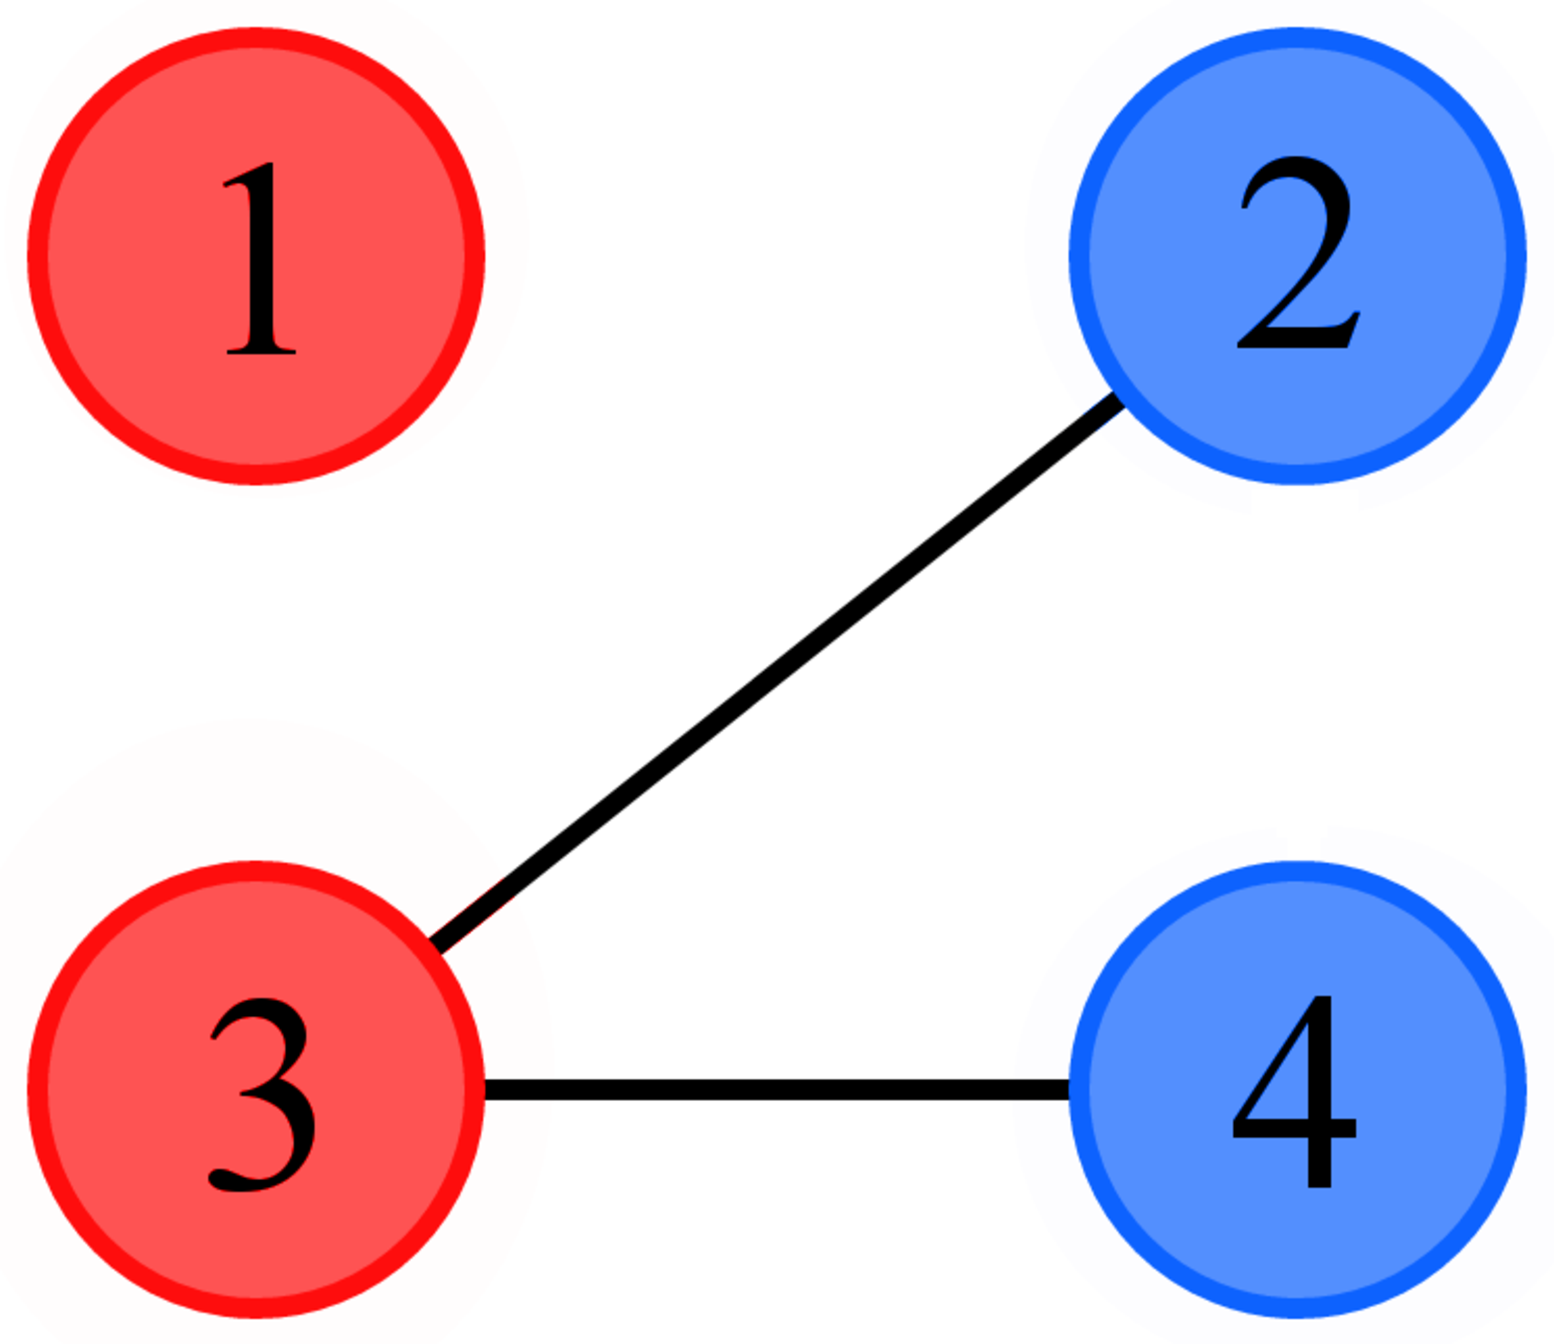
\includegraphics[width=3cm]{../figures/examples-1-incorrect-3-corrected.pdf}
        \end{figure}
        }

        \centering
        Vertex 3 does not have a unique color in its neighborhood.
      \end{column}
    \end{columns}

  \end{frame}

  % \addtocontents{toc}{\protect\vspace{14pt}}

  \subsection{Applications}

  \addtocontents{toc}{\protect\vspace{21pt}}

  \begin{frame}
    \frametitle{Wireless Networks}

    \begin{itemize}
      \item \textbf{Wireless networks} such as cellular networks, television broadcasts, and satellite communication systems can all benefit from conflict-free coloring.

      \begin{figure}[h]
        \centering
        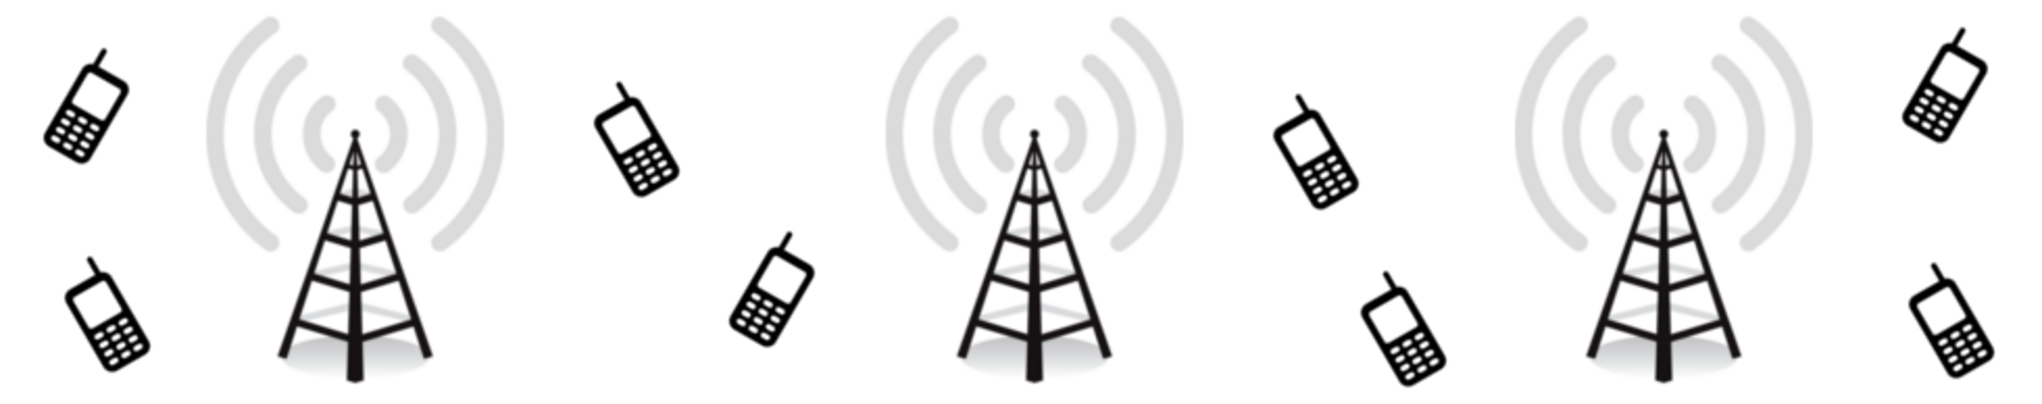
\includegraphics[width=12cm]{../figures/towers-slides.pdf}
      \end{figure}

      \pause

      \item A \textbf{cellular network} is a heterogeneous network with two types of nodes.

      \pause

      \begin{itemize}
        \item Base-stations act as servers and are interconnected by an external backbone network.
        \pause
        \item Clients connect to base-stations via radio links. They constantly search for base-stations with strong reception.
      \end{itemize}
    \end{itemize}

  \end{frame}

  \begin{frame}
    \frametitle{Cellular Networks}

    \begin{itemize}
      \item The problem when designing cellular networks: \textbf{frequency assignment}.
      \begin{itemize}
        \item Imagine two nearby base-stations having the same frequency.
        \item A client in range of both base-stations would receive mutual interference.
      \end{itemize}
    \end{itemize}

    \pause
    \vspace{-0.2cm}

    \begin{itemize}
      \item This leads us to our goal: Assign frequencies such that:
      \pause
      \begin{itemize}
        \item[(1)] Every client is served by a base-station with a unique frequency.
        \pause
        \item[(2)] Minimize the number of frequencies used.
      \end{itemize}
    \end{itemize}

    \pause
    \vfill

    \begin{figure}[h]
      \centering
      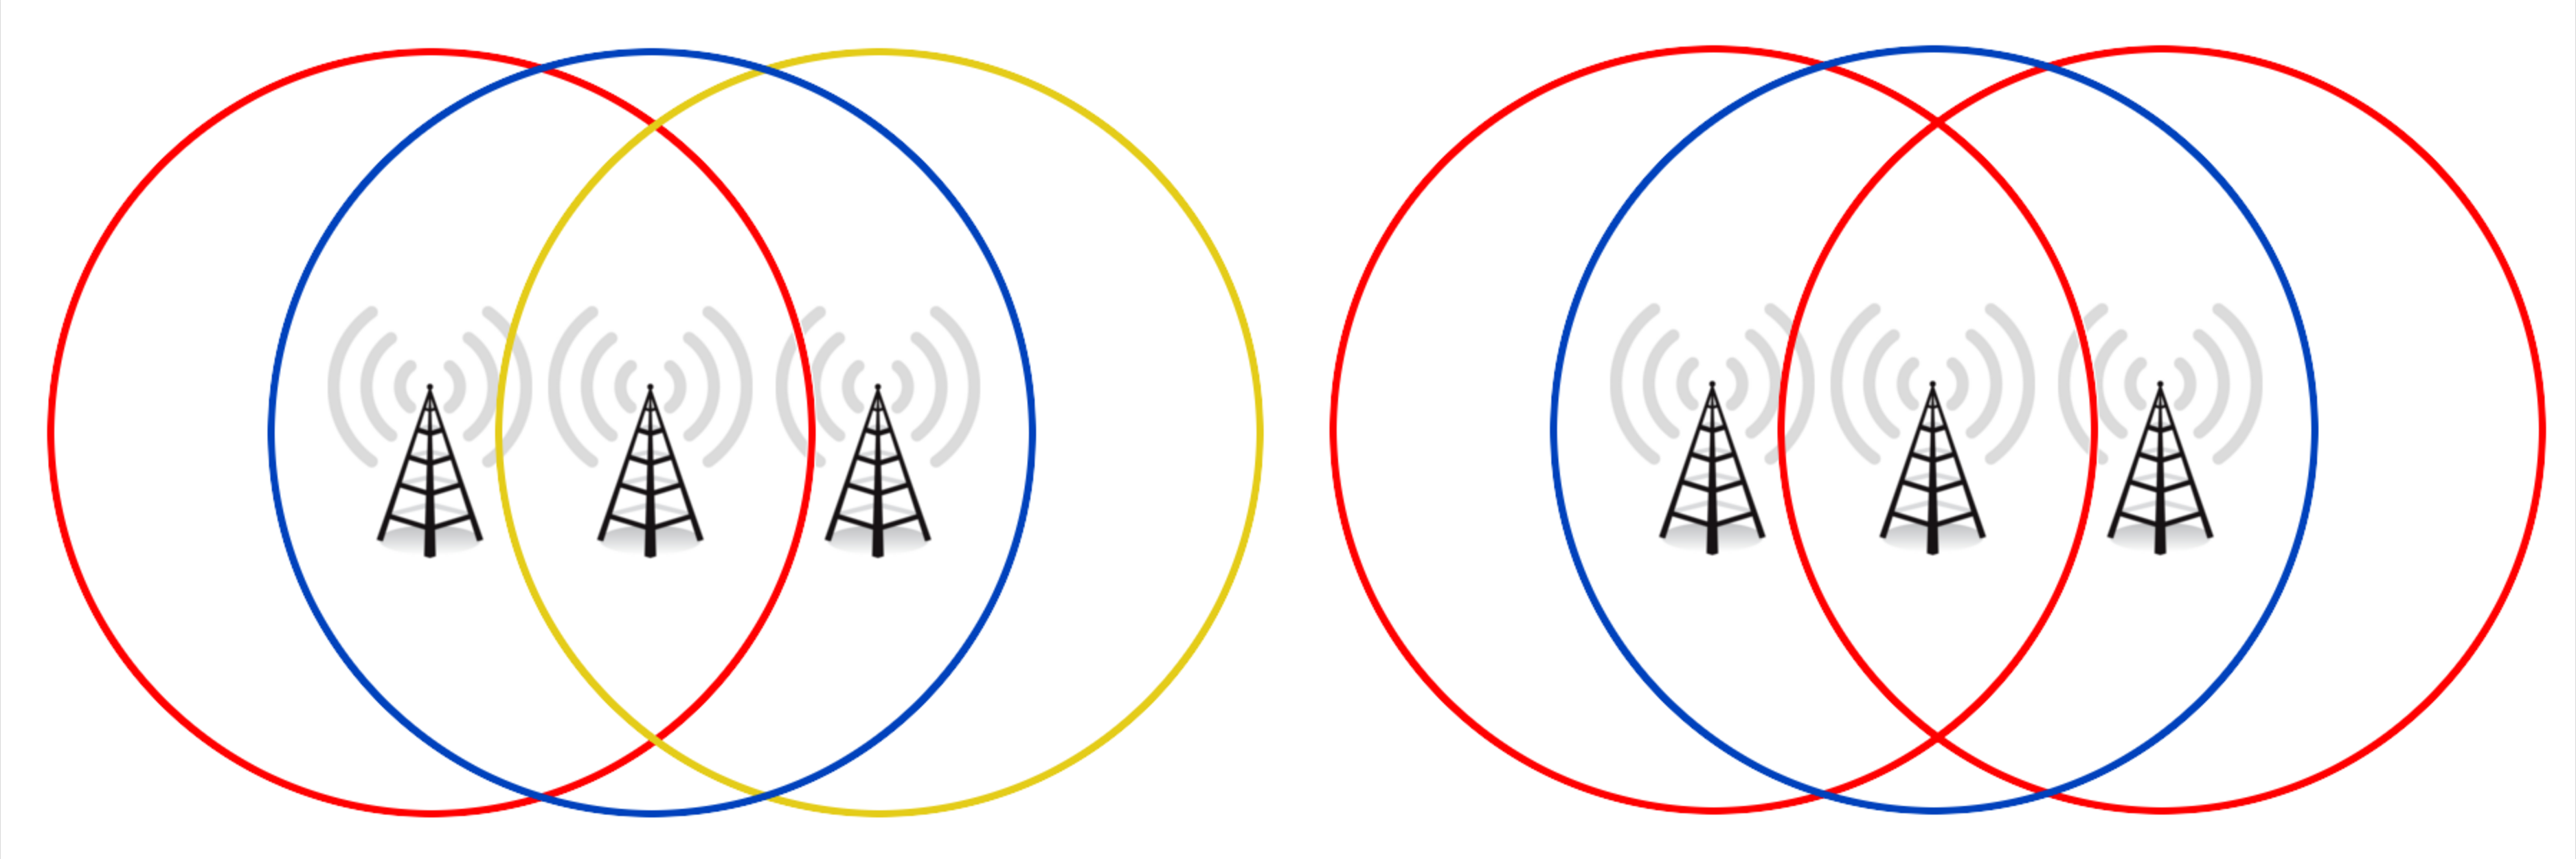
\includegraphics[width=8cm,trim=4 4 4 4,clip]{../figures/towers.pdf}
      \caption*{Vertex coloring and conflict-free coloring of cellular towers, respectively}
    \end{figure}

  \end{frame}

  % \subsection{RFID Networks}
  %
  % \begin{frame}
  %   \frametitle{RFID Networks}
  % \end{frame}

  %

  \addtocontents{toc}{\newpage}


  \section{Coloring for General Graphs}
  \subsection{Guaranteeing k-Colorability}
  \begin{frame}
    \frametitle{Guaranteeing Conflict-Free k-Colorability}

    It is wasteful to spend time coloring a graph that cannot be conflict-free colored within a certain amount of colors ($k$). Thus researchers came up with a criterion to guarantee a graph can be colored with $k$ colors.

    \pause
    \vfill

    A \textbf{complete graph} is a graph where every pair of distinct vertices is connected by an edge.

    \pause

    \begin{itemize}
      \item $K_n$: A complete graph of $n$ vertices.
      \pause
      \item $K_n^{-3}$: A complete graph of $n$ vertices with any three edges forming a triangle removed.
    \end{itemize}

    \pause
    \vfill

    \begin{theorem}
    Let $G$ be a graph and $k \geq 1$. If $G$ has neither $K_{k+2}$ nor $K_{k+3}^{-3}$ as a minor, $G$ has a conflict-free coloring that can be found in polynomial time.
    \end{theorem}

  \end{frame}

  \begin{frame}
    \frametitle{Guaranteeing Conflict-Free k-Colorability}

    % \begin{textblock*}{\examplewidth}(1cm,1.4cm) % {block width} (coords)
    % \end{textblock*}




    \begin{textblock*}{14cm}(1cm, 1.6cm) % {block width} (coords)
      Let's demonstrate meeting this criterion on a graph for the simplest case, $k=1$:
    \end{textblock*}


    \begin{textblock*}{15cm}(0.5cm, 2.1cm) % {block width} (coords)
      \only<1>{
        \begin{figure}
         \centering
         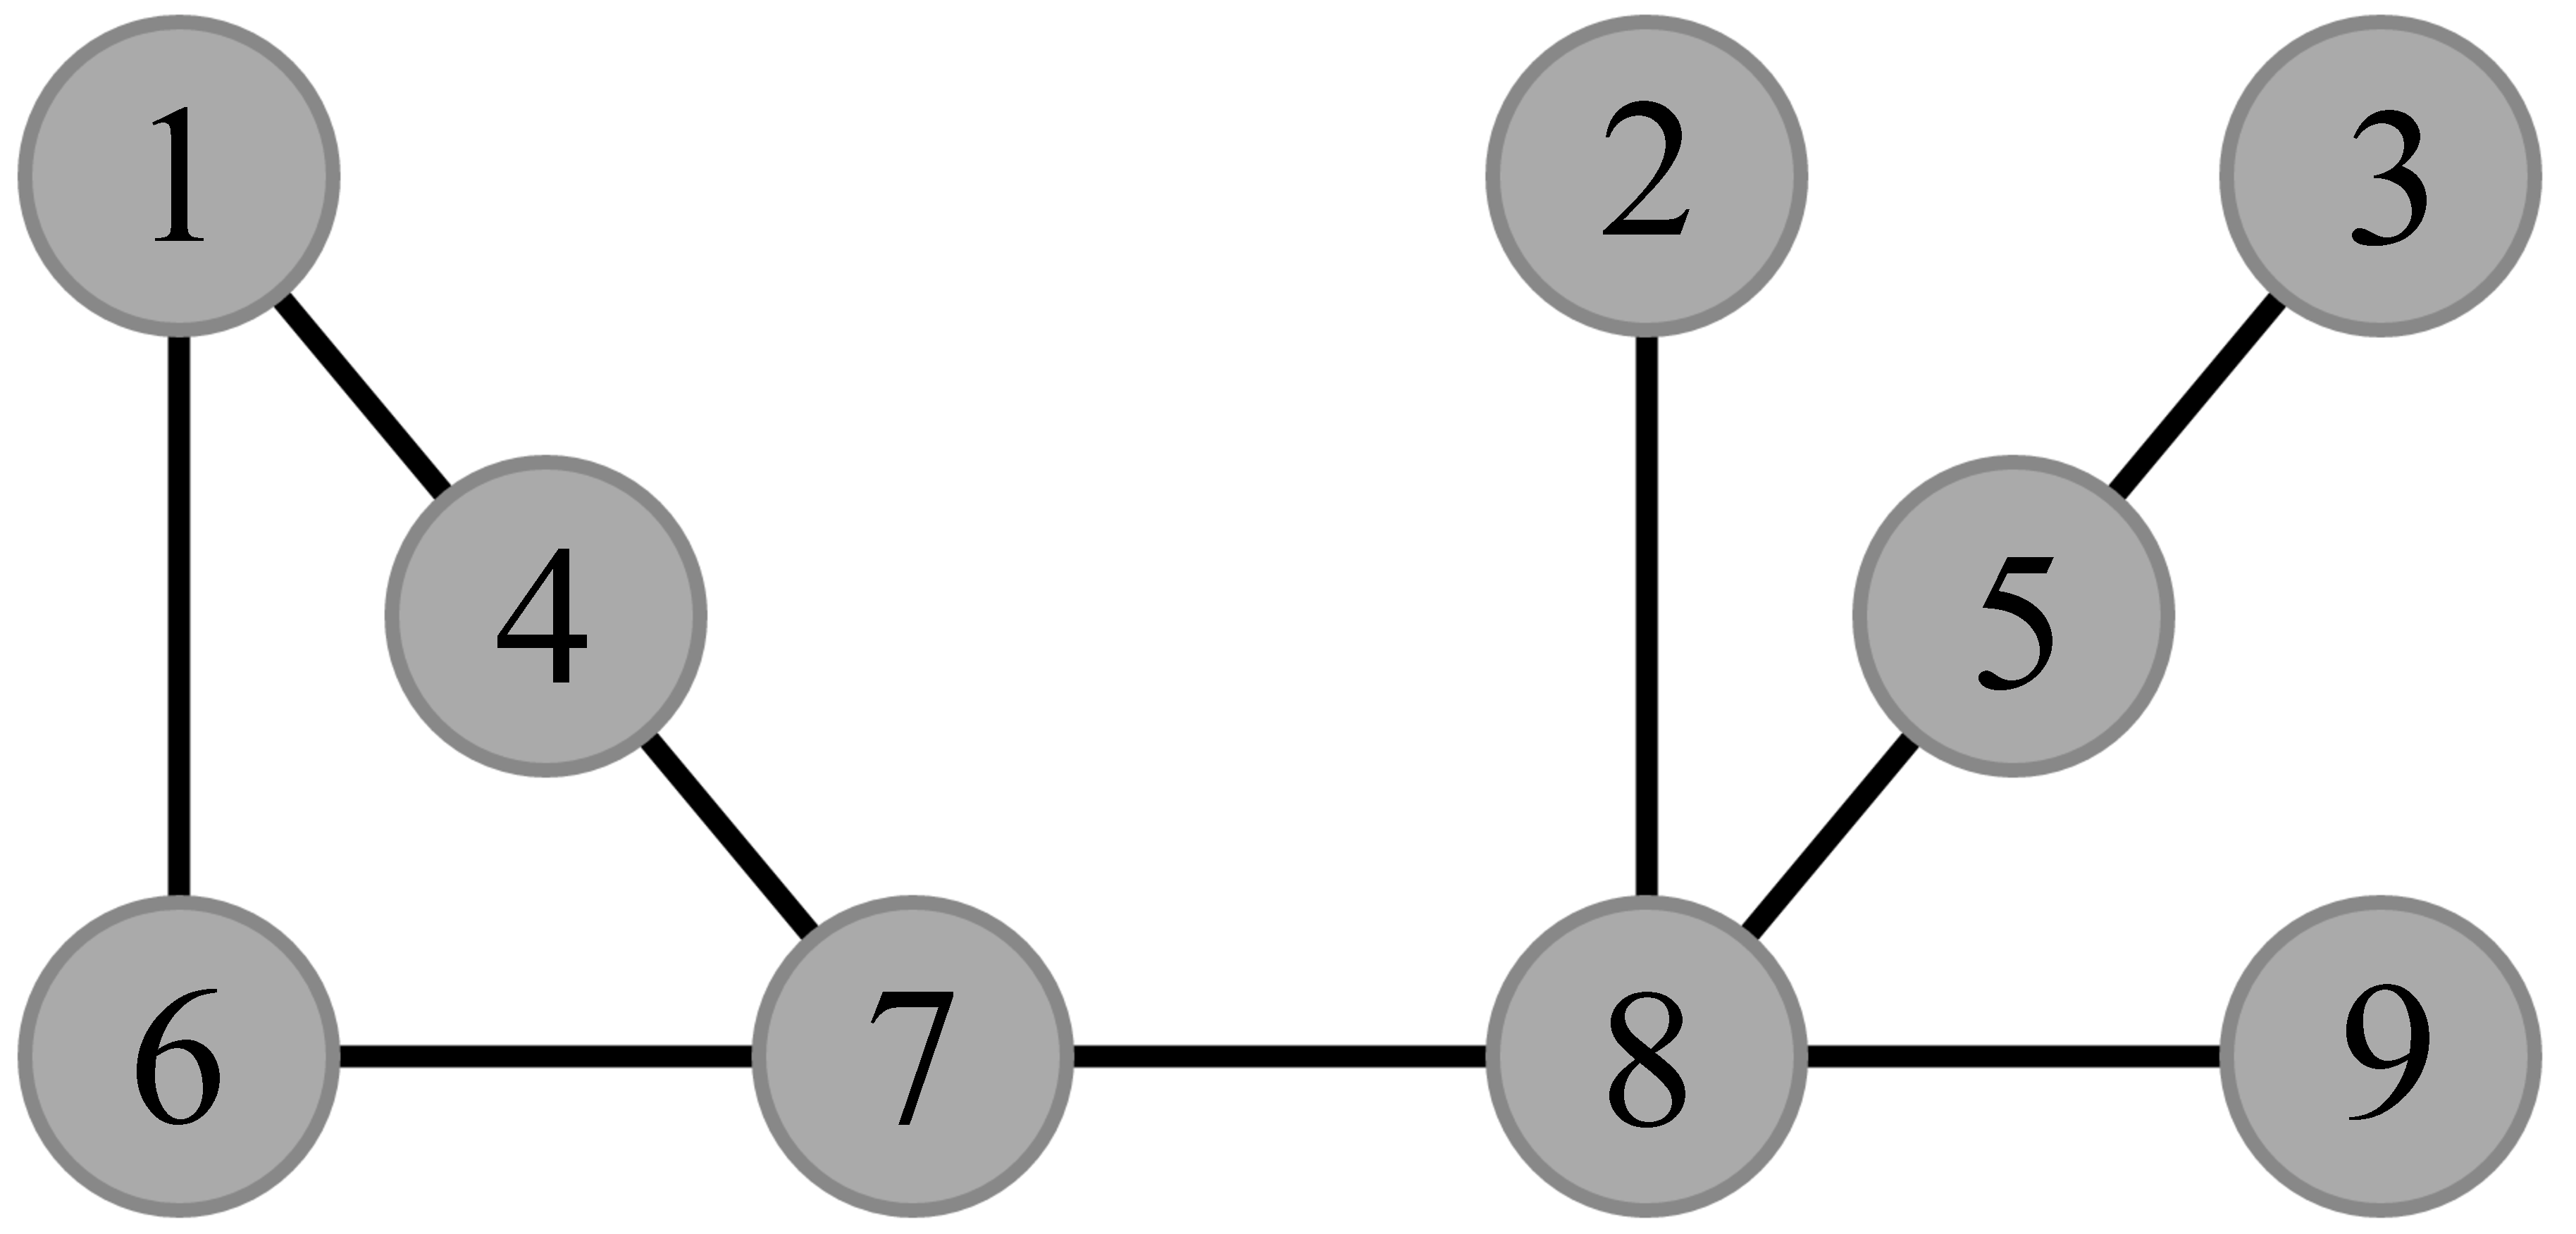
\includegraphics[width=6cm]{../figures/criterion.pdf}
         \caption*{A simple, undirected graph $G$}
       \end{figure}
      }

      \only<2>{
        \vspace{0.25cm}
        \begin{columns}
          \begin{column}{0.5\textwidth}
            \begin{center}
              \begin{figure}
                 \centering
                 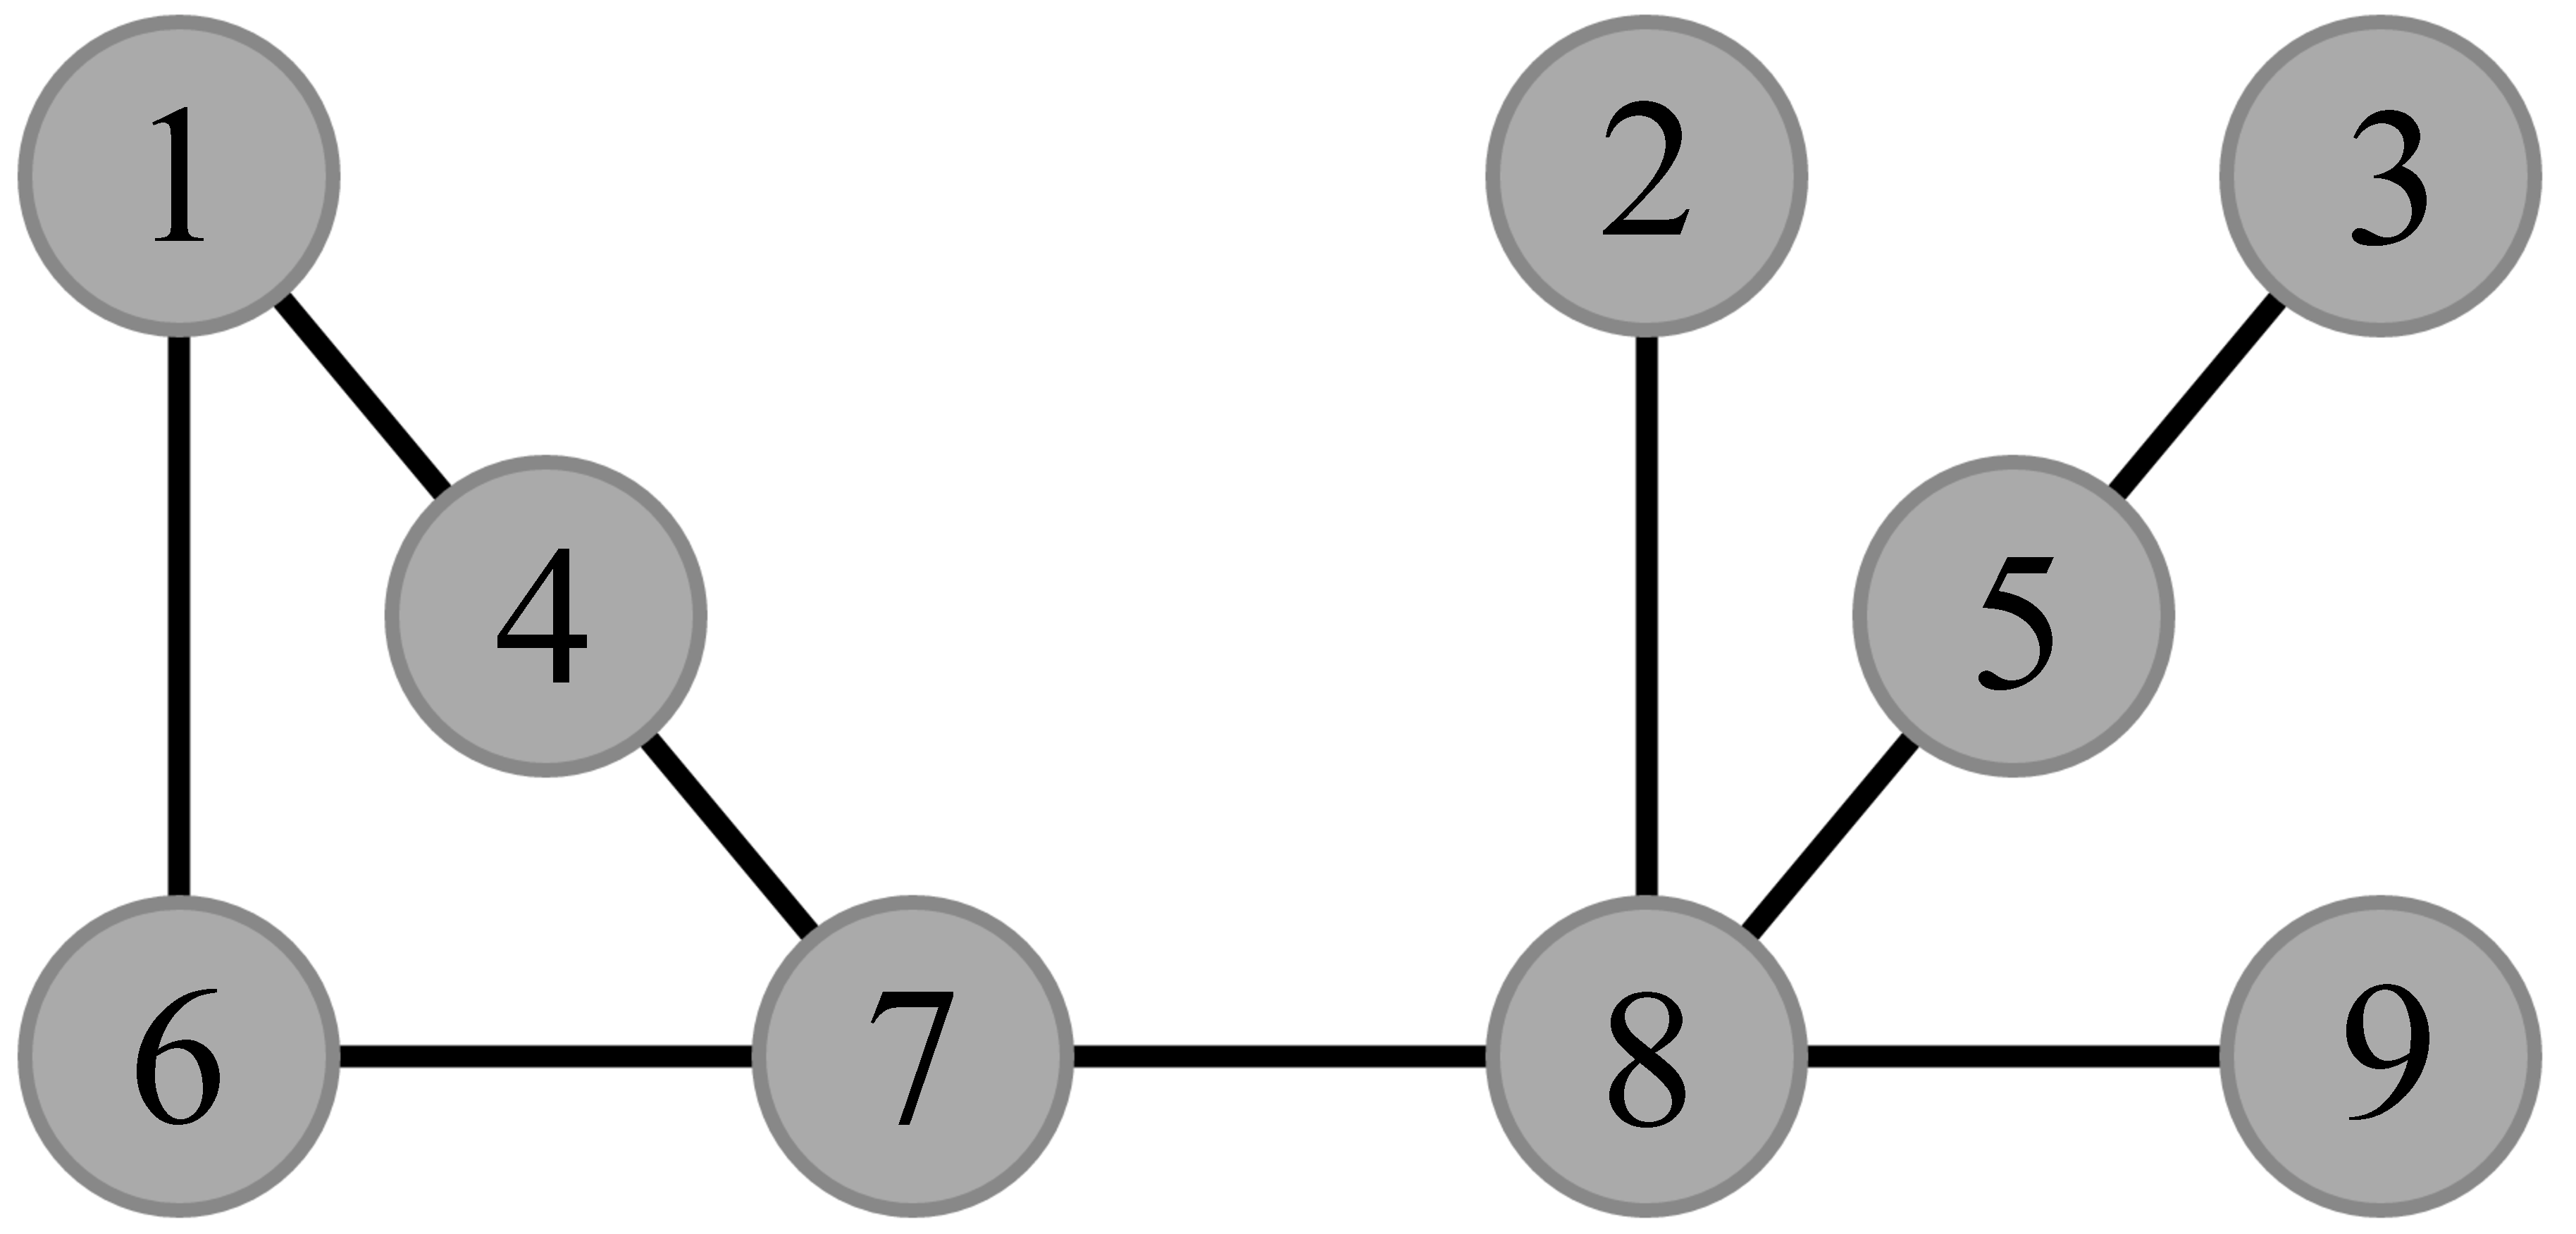
\includegraphics[width=6cm]{../figures/criterion.pdf}
                 \caption*{A simple, undirected graph $G$}
               \end{figure}
            \end{center}
          \end{column}
          \begin{column}{0.5\textwidth}
            \begin{center}
              \begin{figure}
                \centering
                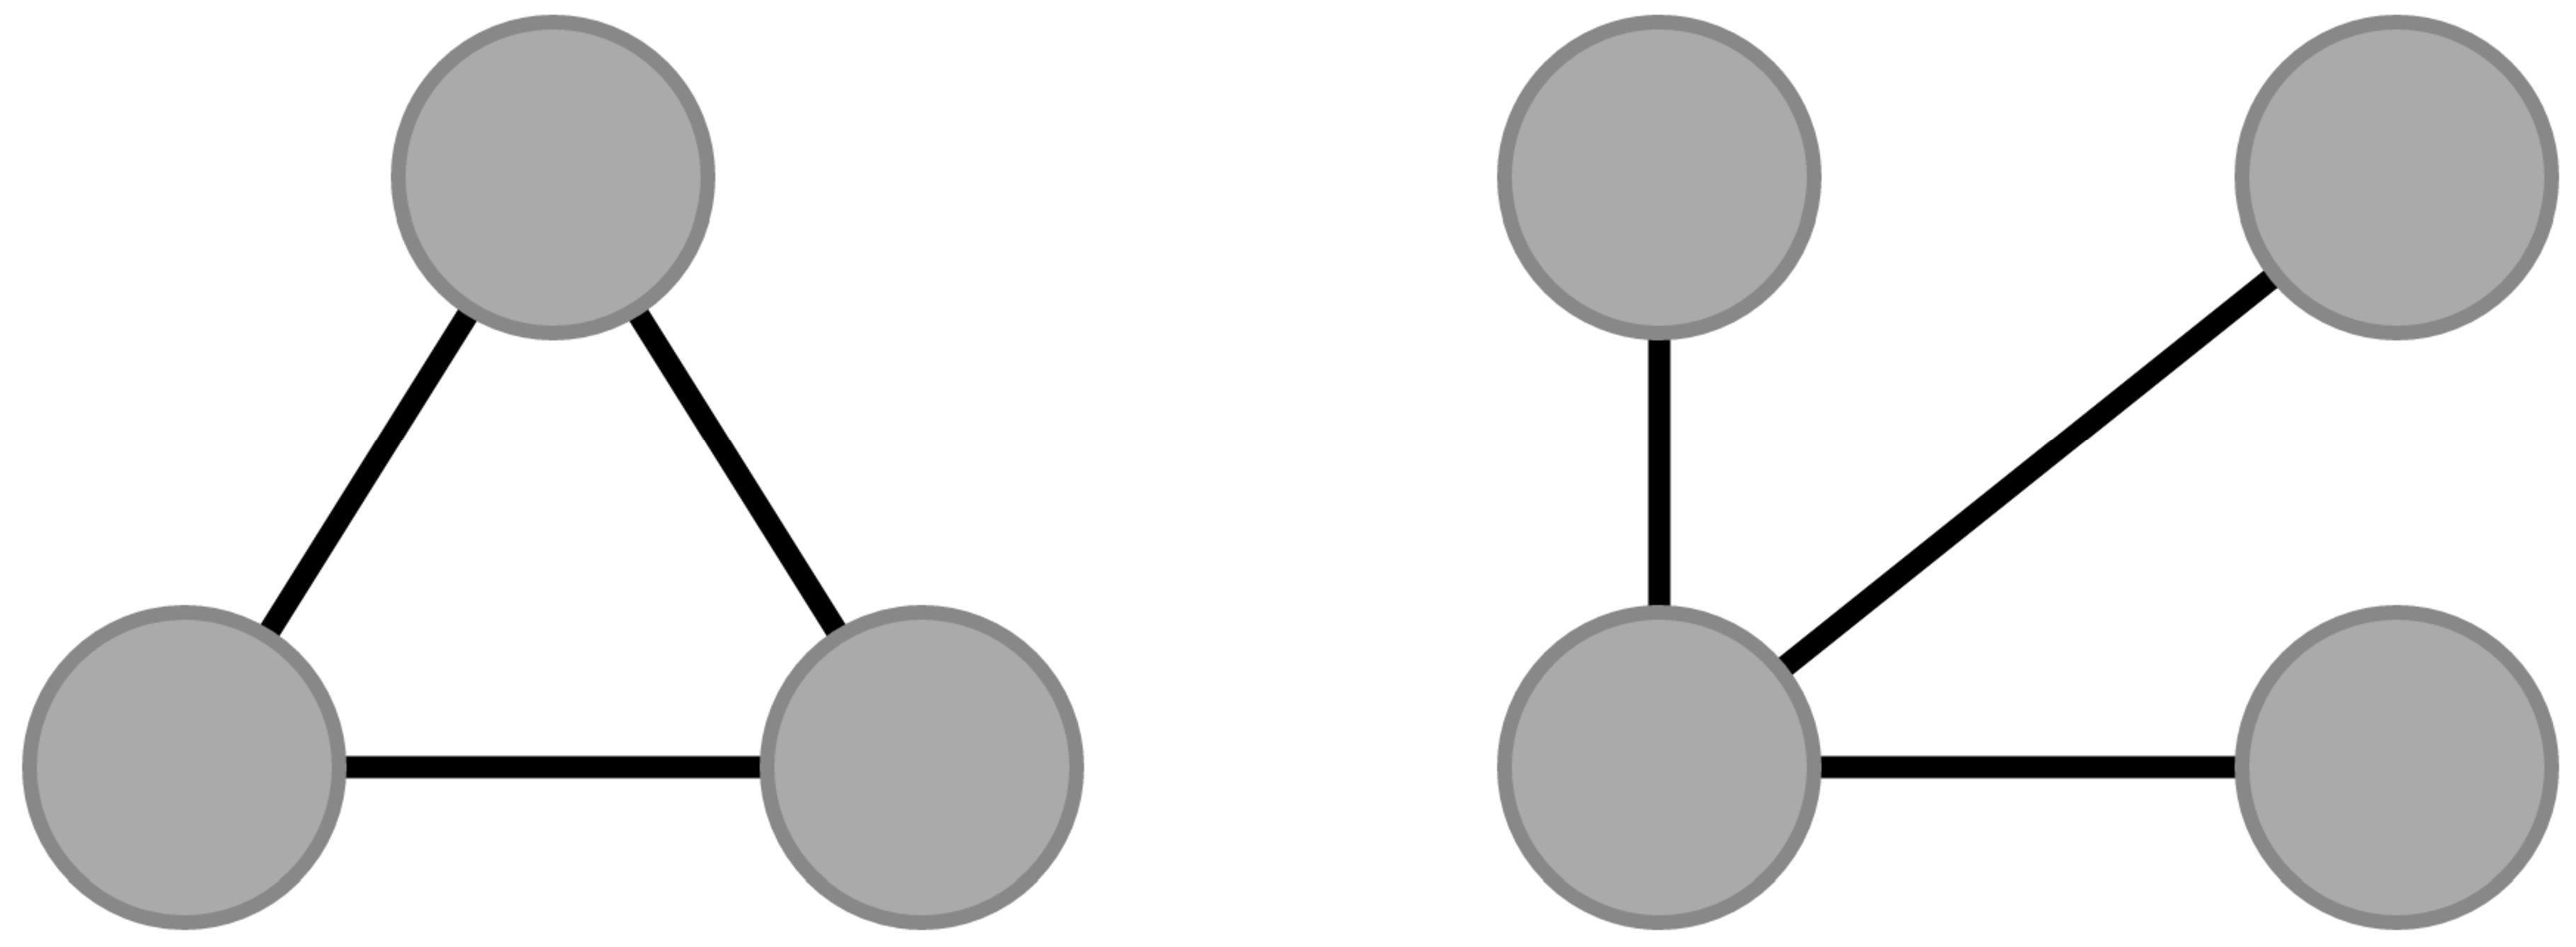
\includegraphics[width=6cm]{../figures/bad-criterion.pdf}
                \caption*{Graphs $K_{3}$ and $K_{4}^{-3}$}
              \end{figure}
            \end{center}
          \end{column}
        \end{columns}
      }

      \only<3>{
        \vspace{0.25cm}
        \begin{columns}
          \begin{column}{0.5\textwidth}
            \begin{center}
              \begin{figure}
                 \centering
                 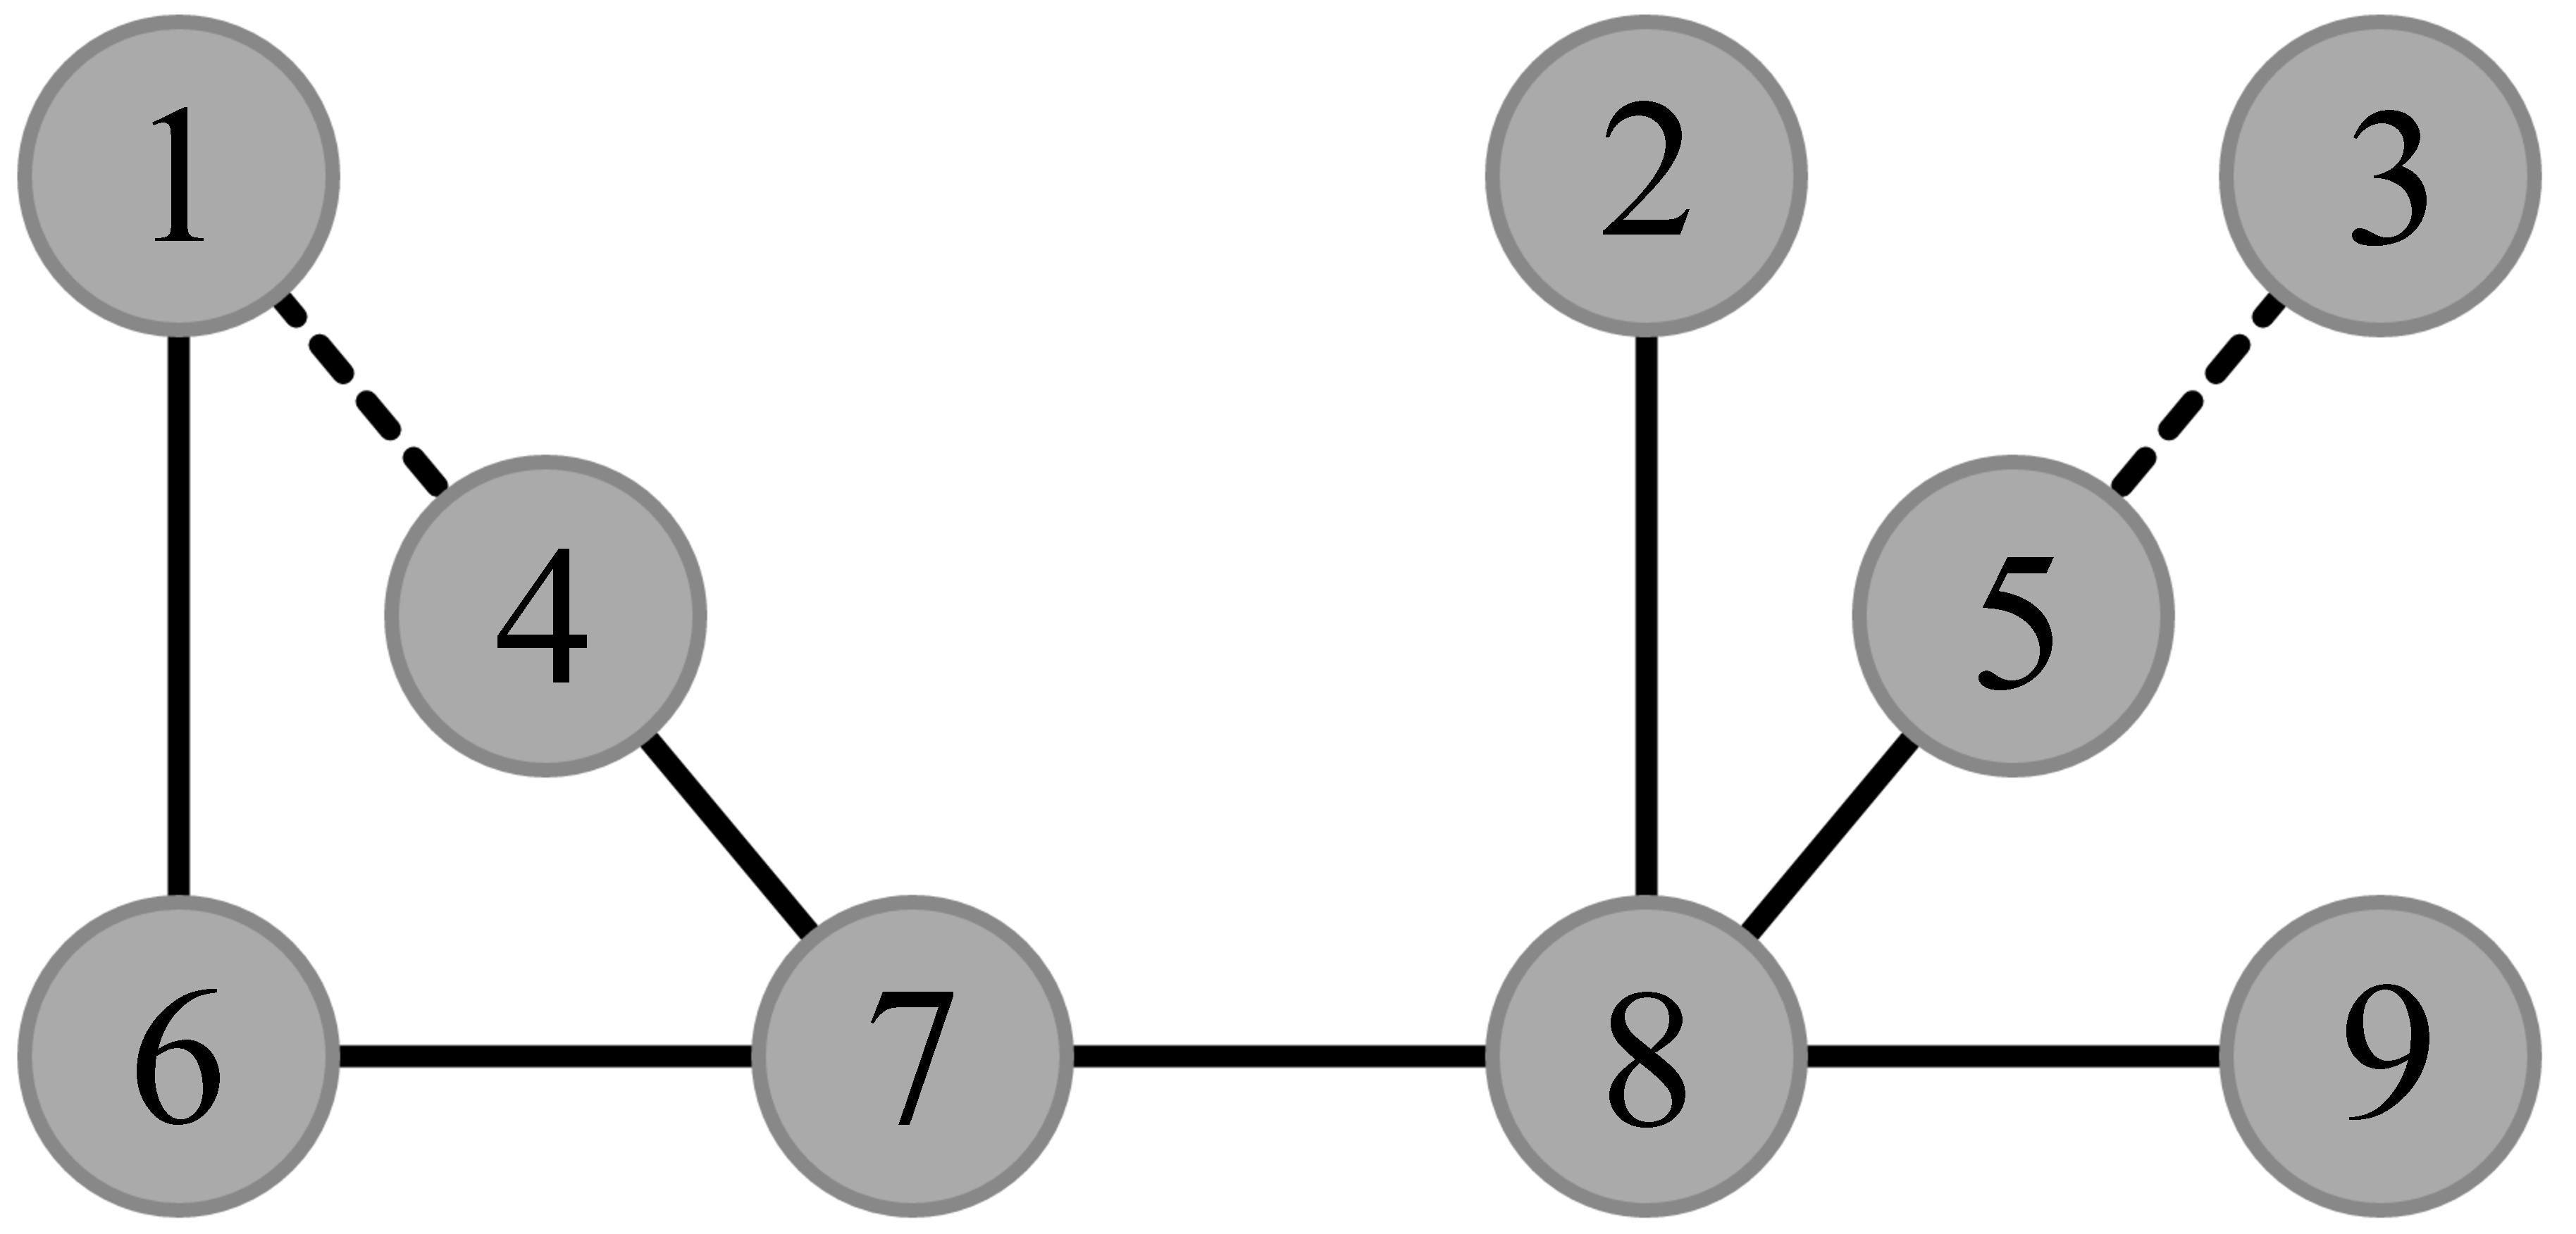
\includegraphics[width=6cm]{../figures/criterion-minor.pdf}
                 \caption*{A simple, undirected graph $G$}
               \end{figure}
            \end{center}
          \end{column}
          \begin{column}{0.5\textwidth}
            \begin{center}
              \begin{figure}
                \centering
                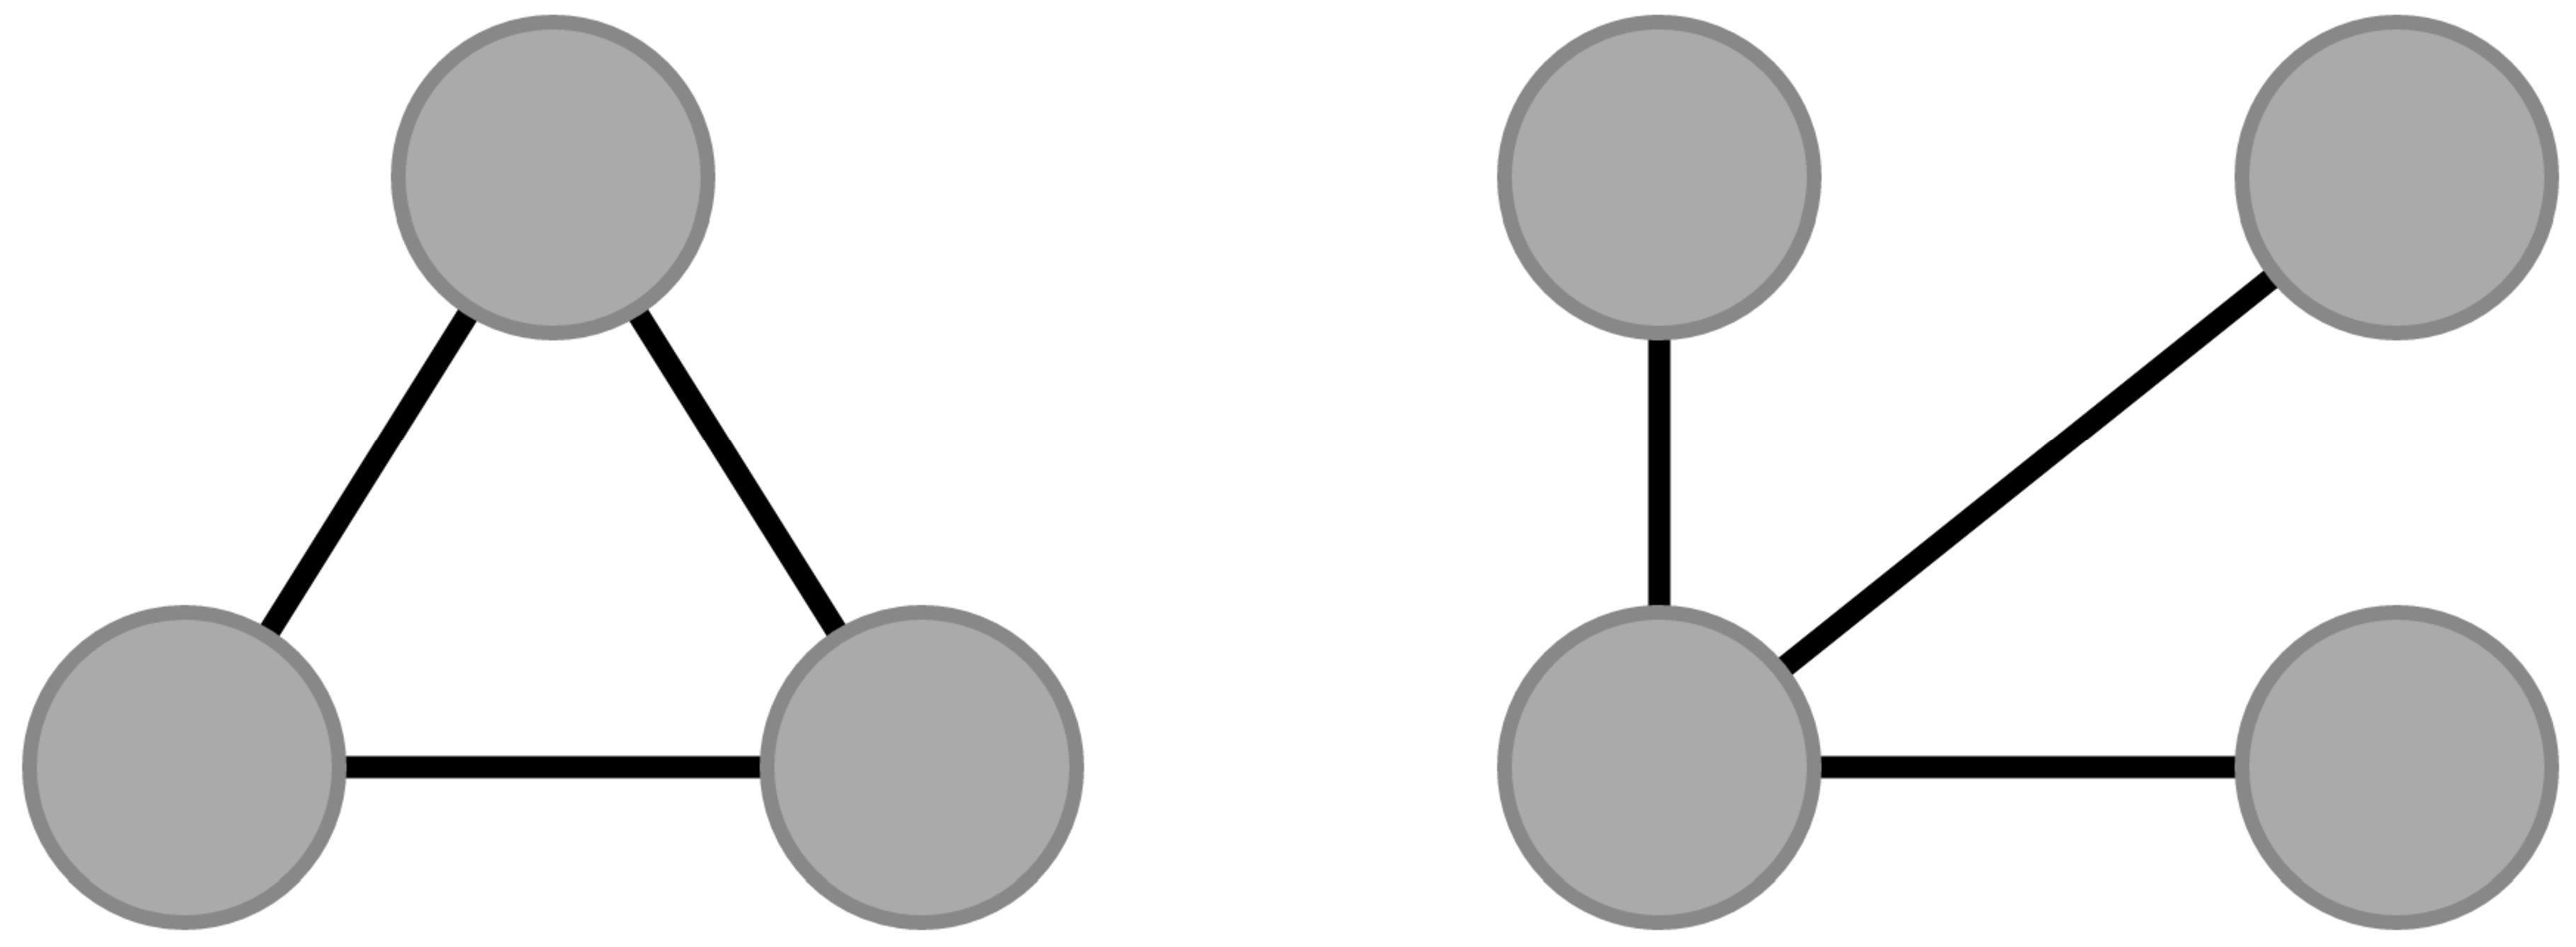
\includegraphics[width=6cm]{../figures/bad-criterion.pdf}
                \caption*{Graphs $K_{3}$ and $K_{4}^{-3}$}
              \end{figure}
            \end{center}
          \end{column}
        \end{columns}
      }
    \end{textblock*}

    \begin{textblock*}{14cm}(1cm, 7.1cm) % {block width} (coords)
      To be conflict-free colored with 1 color, graph $G$ cannot contain $K_3$ or $K_4^{-3}$ as a minor. A graph is a \textbf{minor} if it can be formed by deleting and/or contracting edges from its parent graph. \only<3>{$G$ contains both $K_3$ and $K_4^{-3}$ as a minor and thus {\color{red}\textbf{cannot}} be conflict-free colored with 1 color.}
    \end{textblock*}

  \end{frame}

  \subsection{Distance-3-Sets Algorithm}

  \begin{frame}
    \frametitle{Iterated Elimination of Distance-3-Sets}

    \begin{textblock*}{8cm}(0cm, 8.65cm) % {block width} (coords)
  \begin{center}
    \small
    Colors: $\{1:red,\ 2:blue\}$
  \end{center}
\end{textblock*}

\begin{textblock*}{8cm}(8cm, 7cm) % {block width} (coords)
  \begin{center}
    \only<2-8>{
    $i= 1$
    }

    \only<9-13>{
    $i=2$
    }
  \end{center}
\end{textblock*}

\begin{textblock*}{8cm}(8cm, 7.5cm) % {block width} (coords)
  \only<2-10>{
    \begin{center}
      $P = \{\}$
    \end{center}
  }

  \only<11-13>{
    \begin{center}
      $P = \{\{5\},\{7\}\}$
    \end{center}
  }
\end{textblock*}

\only<1>{
  \begin{columns}
    \begin{column}{0.5\textwidth}
      \begin{algorithm}[H]
        \caption*{\textbf{Algorithm} IEDS}
        \scriptsize
        \begin{algorithmic}[1]
        \State $i \gets 1,\ P \gets \emptyset$
        \State Remove all isolated paths from $G$
        \While{$G$ is not empty}
          \State $D \gets \emptyset$
          \ForAll{components of $G$}
            \State Pick any vertex $v$
            \State $D \gets D \cup \{ v \}$
            \While{$\exists u$ at distance $\geq 3$ $\forall v \in D$}
              \State Pick $u$ at distance 3 from some vertex in $D$
              \State $D \gets D \cup \{ w \}$
            \EndWhile
            \ForAll{$u \in D$}
              \State Color $u$ with color $i$
            \EndFor
            \State $i \gets i + 1$
            \ForAll{$u \in D$}
              \State Remove $N(u)$ from $G$
            \EndFor
            \State Remove all isolated paths from G
          \EndFor
        \EndWhile
        \State Color all removed isolated paths using color $i$
        \end{algorithmic}
      \end{algorithm}
    \end{column}
    \begin{column}{0.5\textwidth}
      \begin{center}
        \begin{textblock*}{8cm}(8cm, 1.2cm) % {block width} (coords)
          \begin{figure}
            \centering
            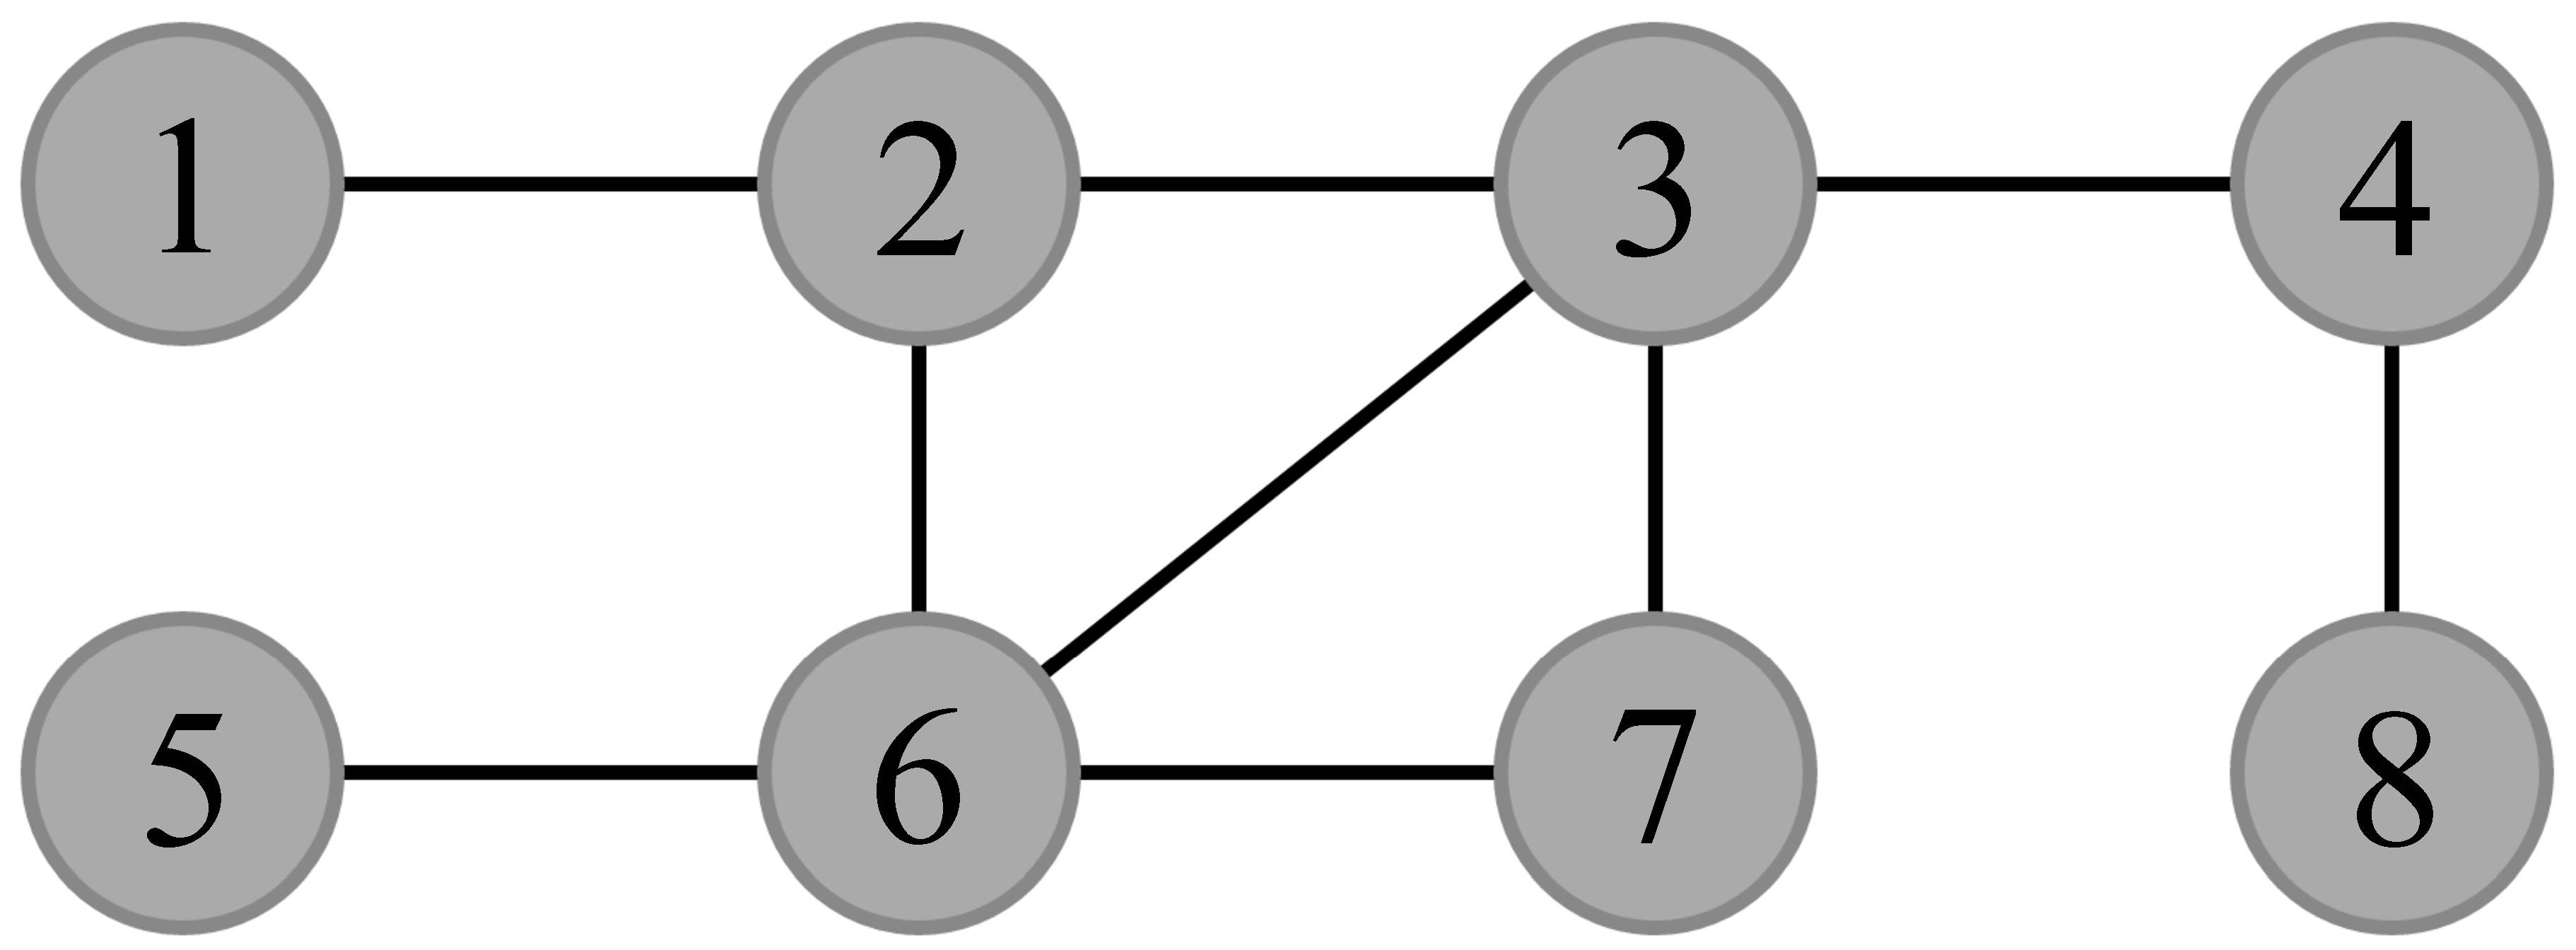
\includegraphics[width=5.7cm]{../figures/algorithm1.pdf}
            \caption*{Coloring of $G$ so far}
          \end{figure}
        \end{textblock*}
        \begin{textblock*}{8cm}(8cm, 4cm) % {block width} (coords)
          \begin{figure}
            \centering
            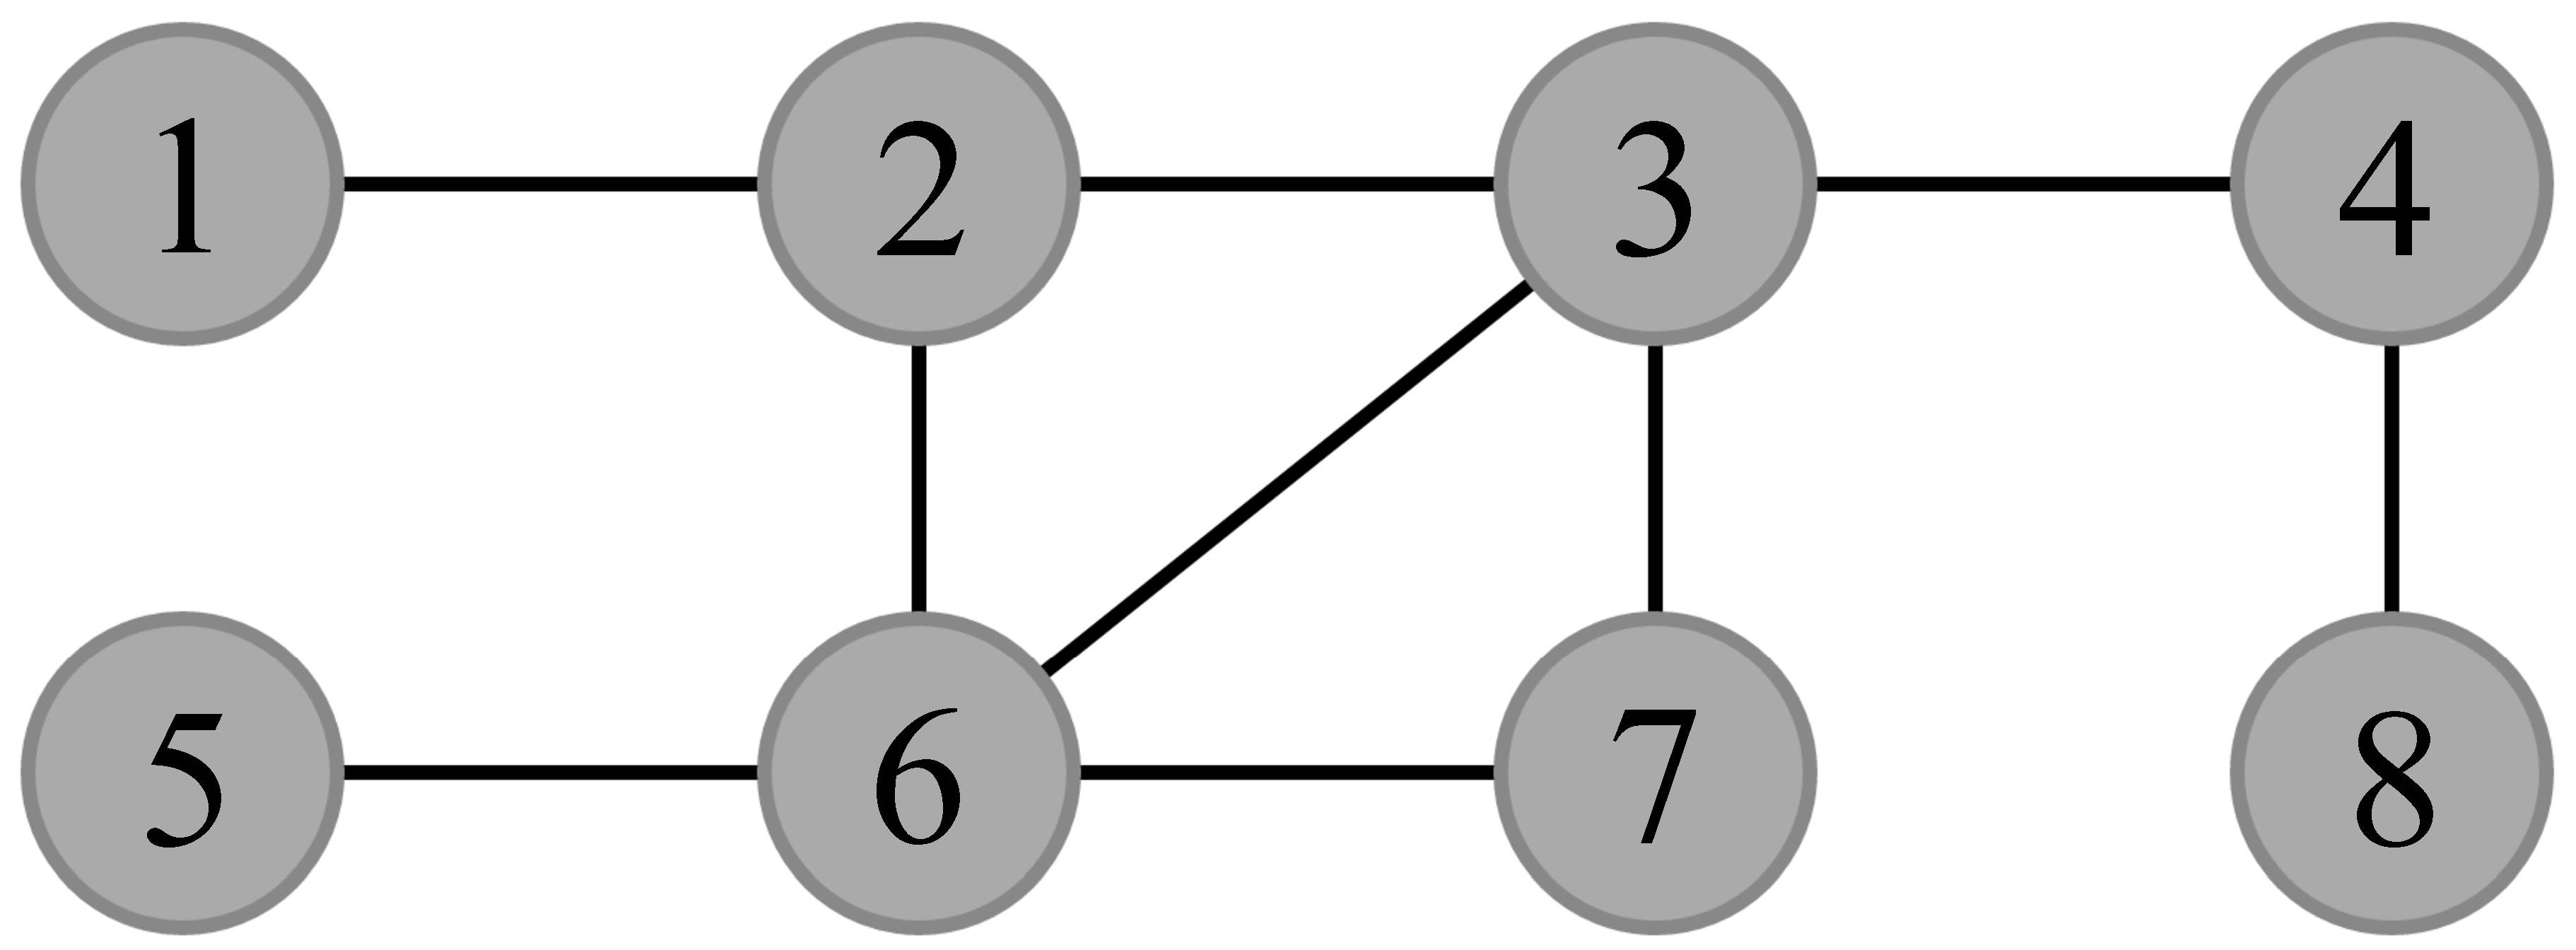
\includegraphics[width=5.7cm]{../figures/algorithm1.pdf}
            \caption*{A simple graph $G$}
          \end{figure}
        \end{textblock*}
      \end{center}
    \end{column}
  \end{columns}
}

\only<2>{
  \begin{columns}
    \begin{column}{0.5\textwidth}
      \begin{algorithm}[H]
        \caption*{\textbf{Algorithm} IEDS}
        \scriptsize
        \begin{algorithmic}[1]
        \CSTATE $i \gets 1,\ P \gets \emptyset$
        \CSTATE Remove all isolated paths from $G$
        \While{$G$ is not empty}
          \State $D \gets \emptyset$
          \ForAll{components of $G$}
            \State Pick any vertex $v$
            \State $D \gets D \cup \{ v \}$
            \While{$\exists u$ at distance $\geq 3$ $\forall v \in D$}
              \State Pick $u$ at distance 3 from some vertex in $D$
              \State $D \gets D \cup \{ w \}$
            \EndWhile
            \ForAll{$u \in D$}
              \State Color $u$ with color $i$
            \EndFor
            \State $i \gets i + 1$
            \ForAll{$u \in D$}
              \State Remove $N(u)$ from $G$
            \EndFor
            \State Remove all isolated paths from G
          \EndFor
        \EndWhile
        \State Color all removed isolated paths using color $i$
        \end{algorithmic}
      \end{algorithm}
    \end{column}
    \begin{column}{0.5\textwidth}
      \begin{center}
        \begin{textblock*}{8cm}(8cm, 1.2cm) % {block width} (coords)
          \begin{figure}
            \centering
            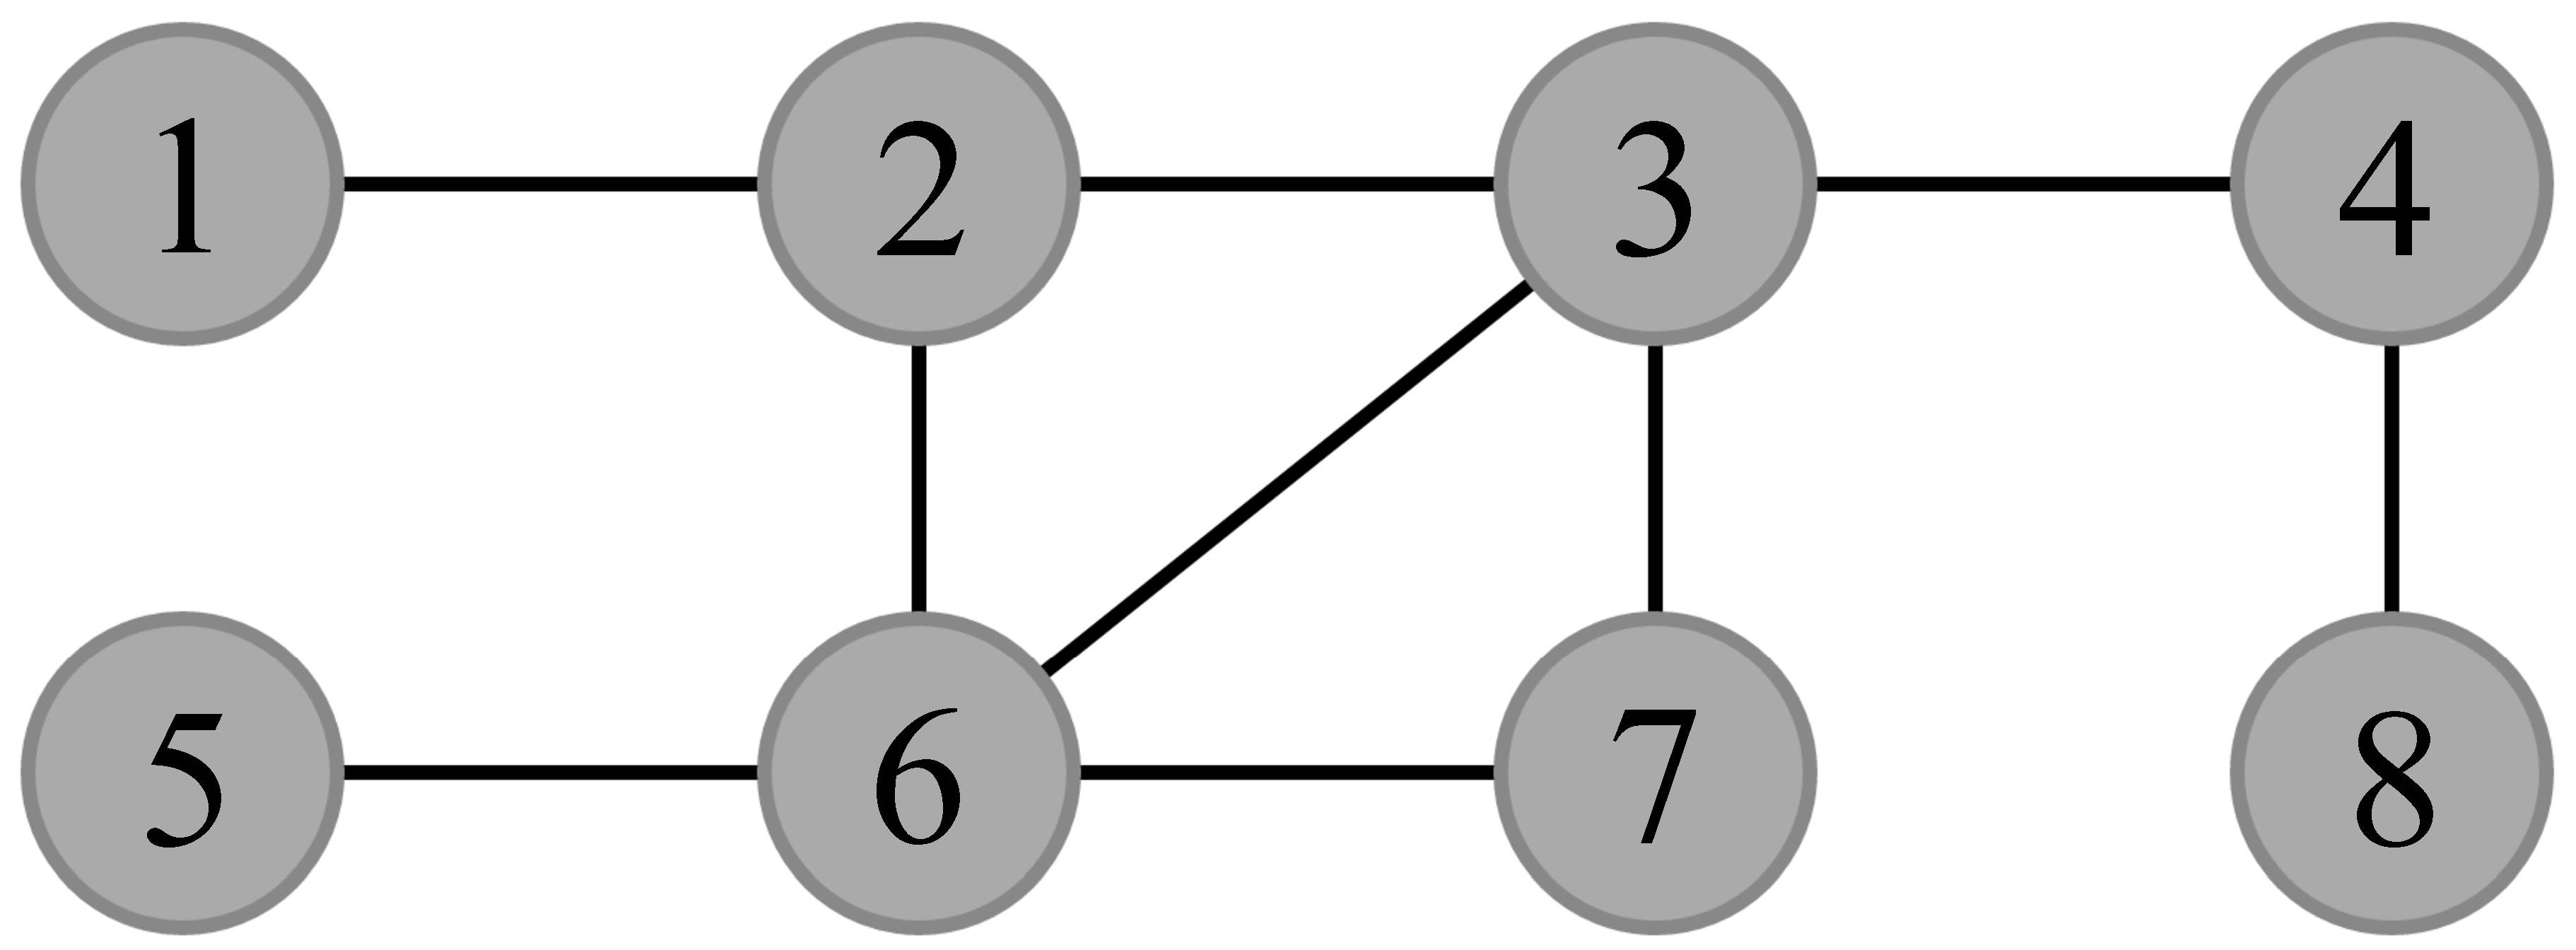
\includegraphics[width=5.7cm]{../figures/algorithm1.pdf}
            \caption*{Coloring of $G$ so far}
          \end{figure}
        \end{textblock*}
        \begin{textblock*}{8cm}(8cm, 4cm) % {block width} (coords)
          \begin{figure}
            \centering
            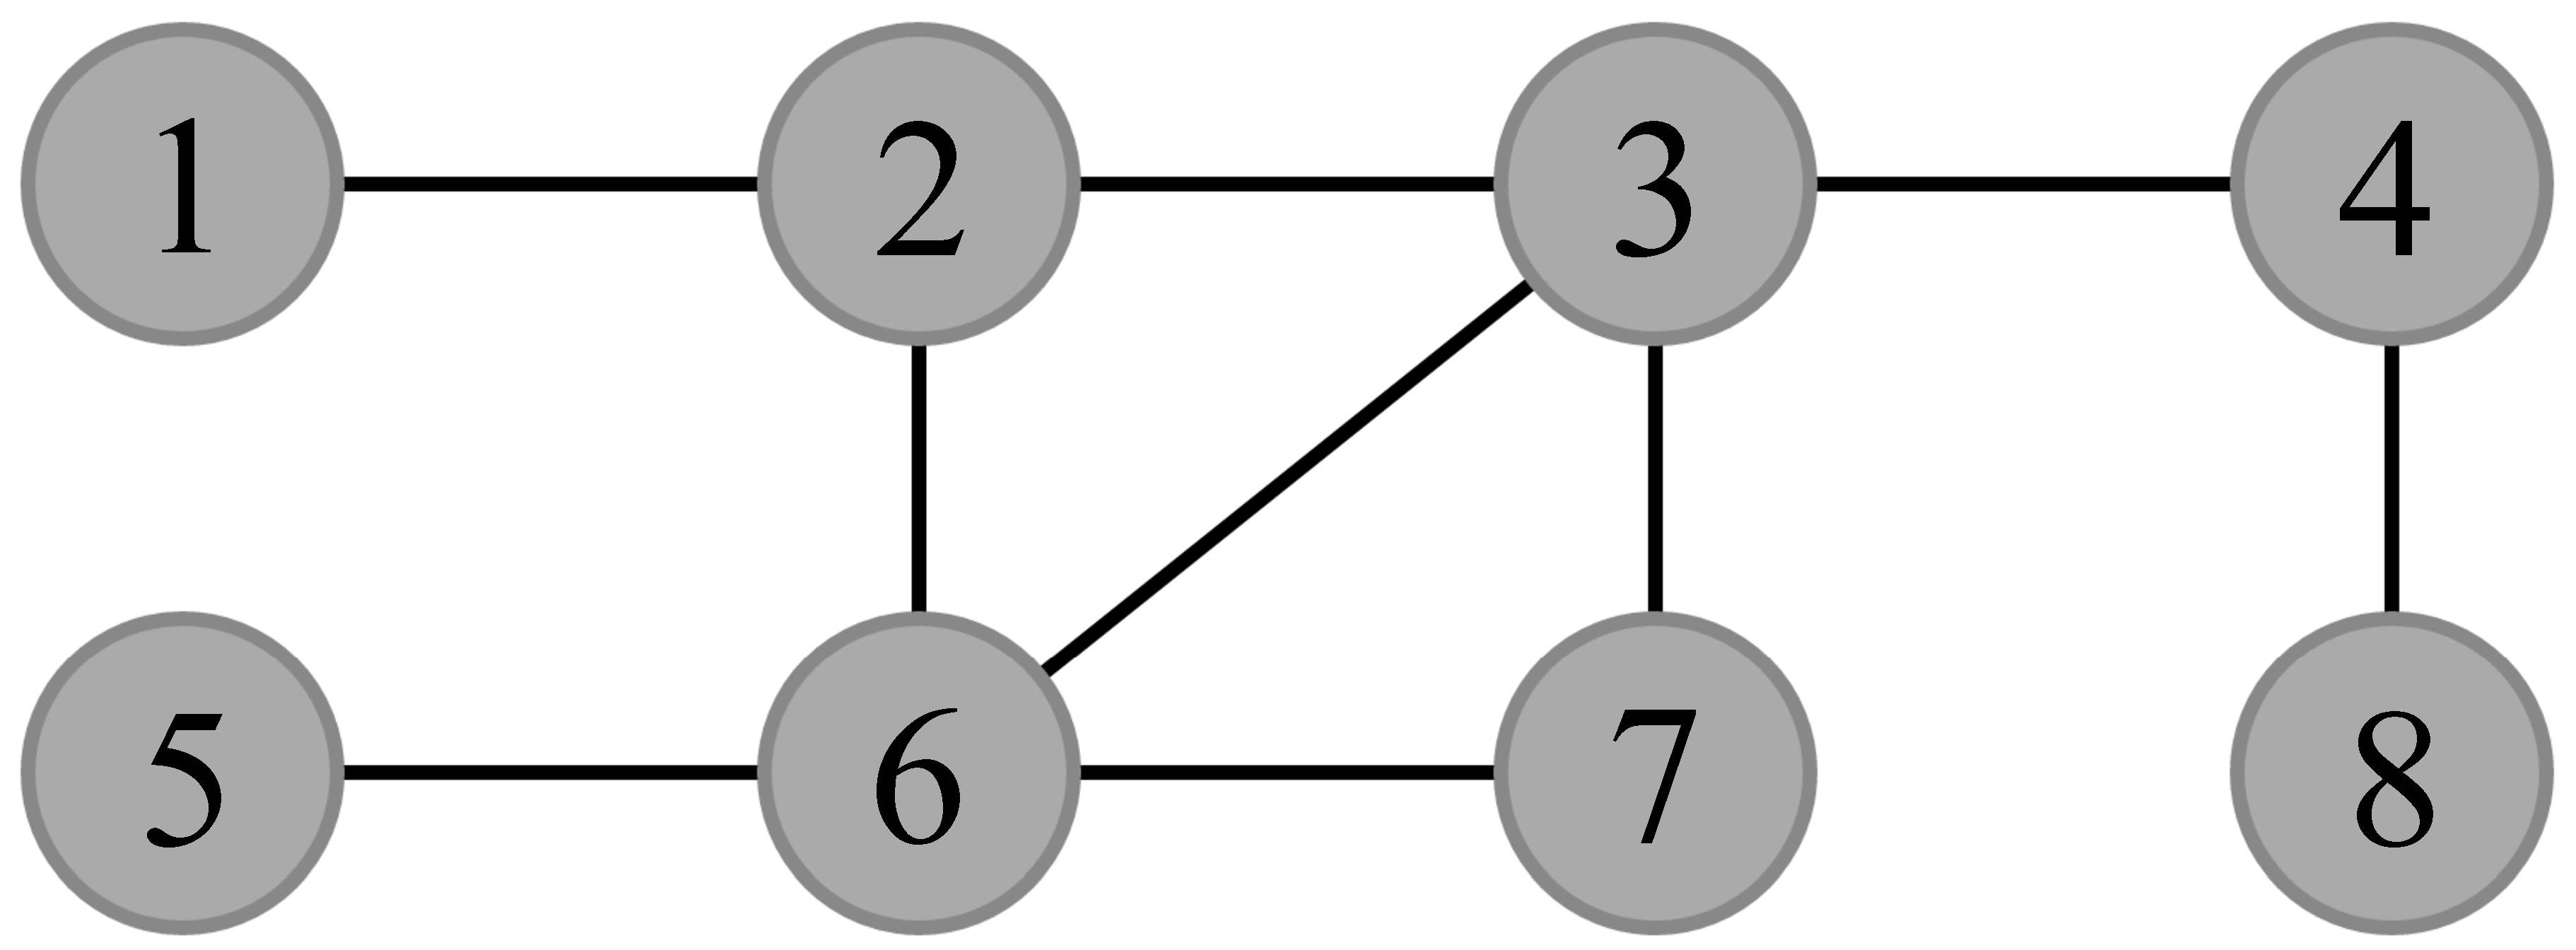
\includegraphics[width=5.7cm]{../figures/algorithm1.pdf}
            \caption*{A simple graph $G$}
          \end{figure}
        \end{textblock*}
      \end{center}
    \end{column}
  \end{columns}
}

\only<3>{
  \begin{textblock*}{8cm}(8cm, 8cm) % {block width} (coords)
    \begin{center}
      $D= \{\}$
    \end{center}
  \end{textblock*}

  \begin{columns}
    \begin{column}{0.5\textwidth}
      \begin{algorithm}[H]
        \caption*{\textbf{Algorithm} IEDS}
        \scriptsize
        \begin{algorithmic}[1]
        \State $i \gets 1,\ P \gets \emptyset$
        \State Remove all isolated paths from $G$
        \While{$G$ is not empty}
          \CSTATE $D \gets \emptyset$
          \ForAll{components of $G$}
            \State Pick any vertex $v$
            \State $D \gets D \cup \{ v \}$
            \While{$\exists u$ at distance $\geq 3$ $\forall v \in D$}
              \State Pick $u$ at distance 3 from some vertex in $D$
              \State $D \gets D \cup \{ w \}$
            \EndWhile
            \ForAll{$u \in D$}
              \State Color $u$ with color $i$
            \EndFor
            \State $i \gets i + 1$
            \ForAll{$u \in D$}
              \State Remove $N(u)$ from $G$
            \EndFor
            \State Remove all isolated paths from G
          \EndFor
        \EndWhile
        \State Color all removed isolated paths using color $i$
        \end{algorithmic}
      \end{algorithm}
    \end{column}
    \begin{column}{0.5\textwidth}
      \begin{center}
        \begin{textblock*}{8cm}(8cm, 1.2cm) % {block width} (coords)
          \begin{figure}
            \centering
            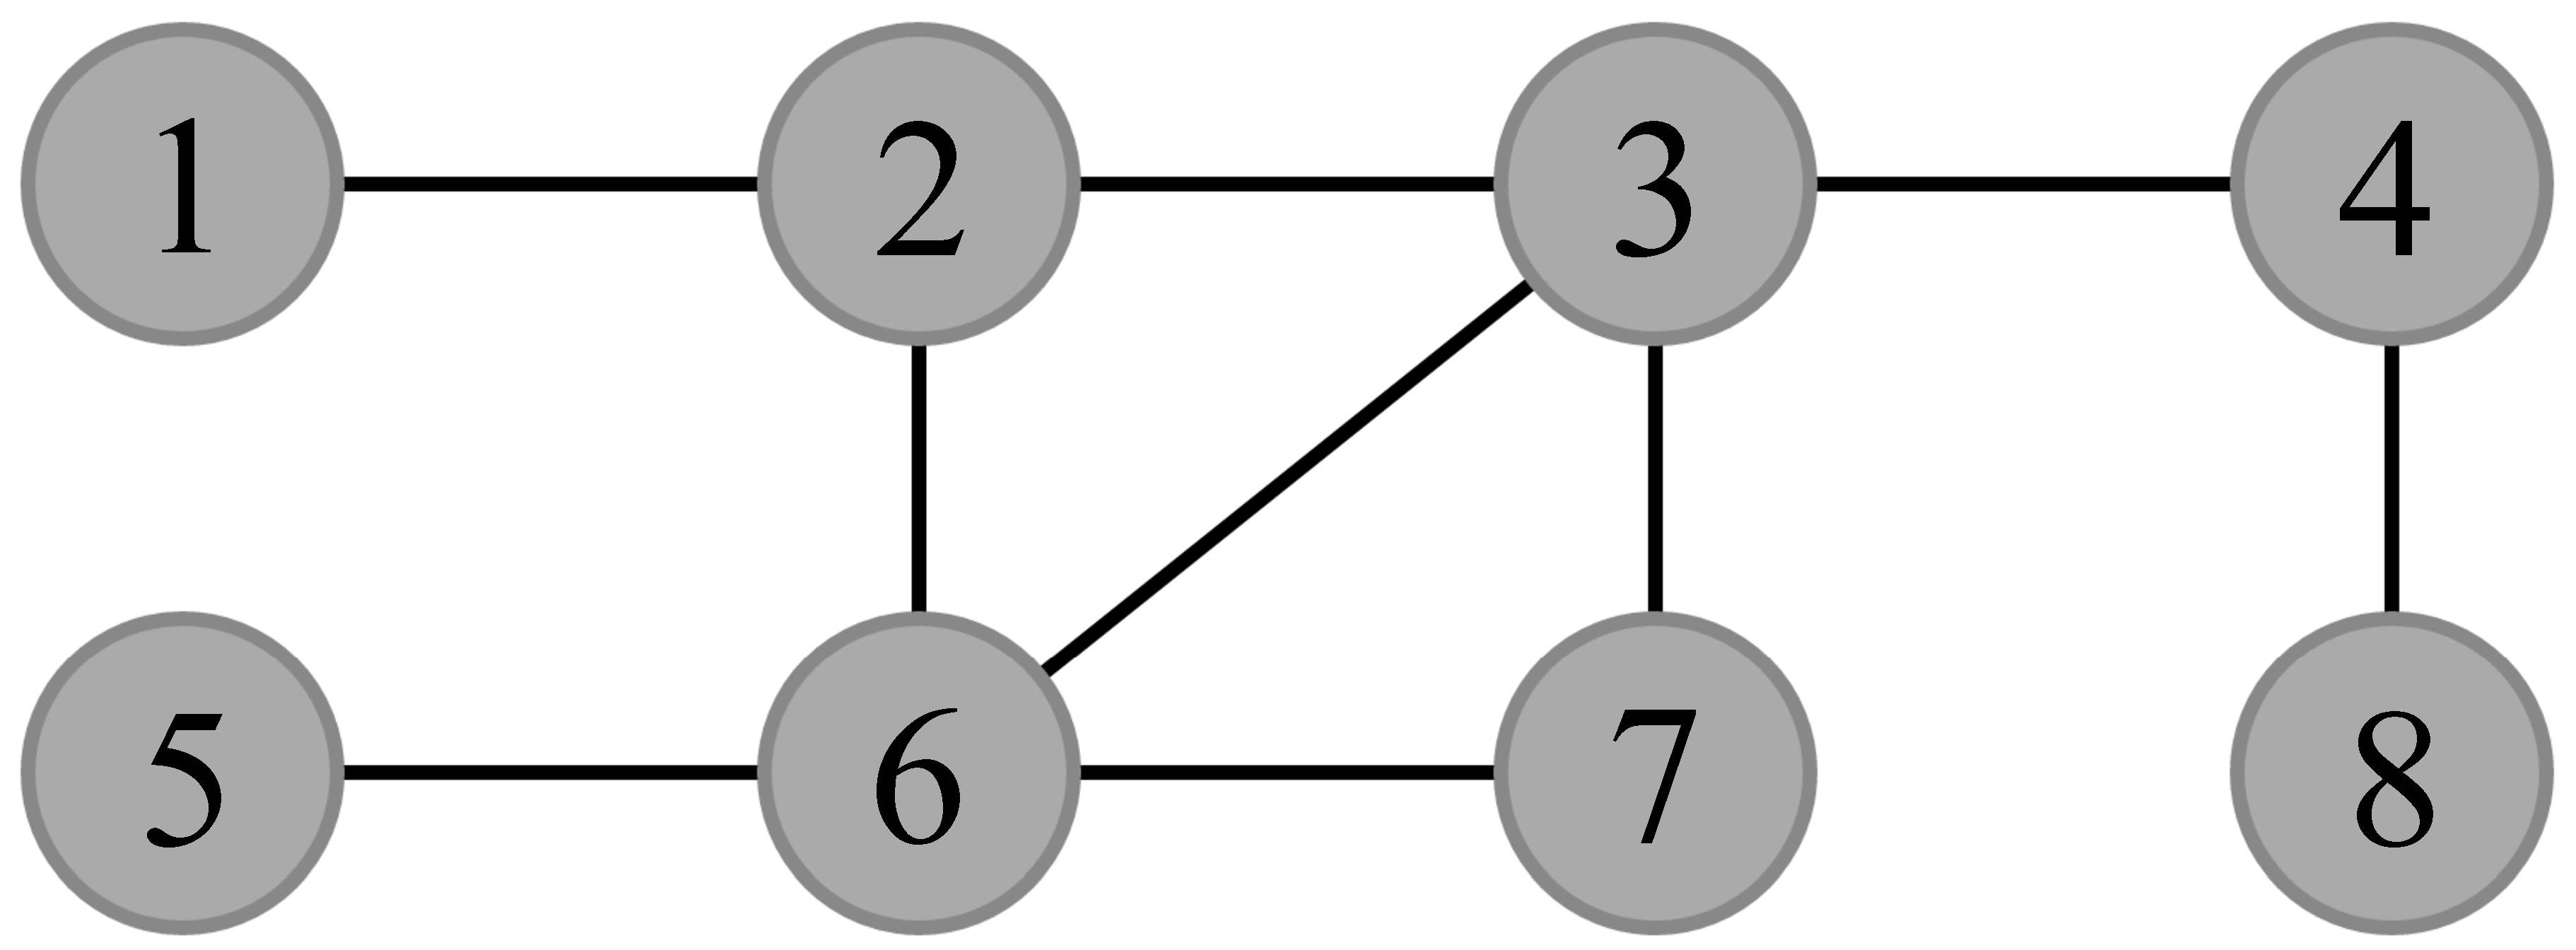
\includegraphics[width=5.7cm]{../figures/algorithm1.pdf}
            \caption*{Coloring of $G$ so far}
          \end{figure}
        \end{textblock*}
        \begin{textblock*}{8cm}(8cm, 4cm) % {block width} (coords)
          \begin{figure}
            \centering
            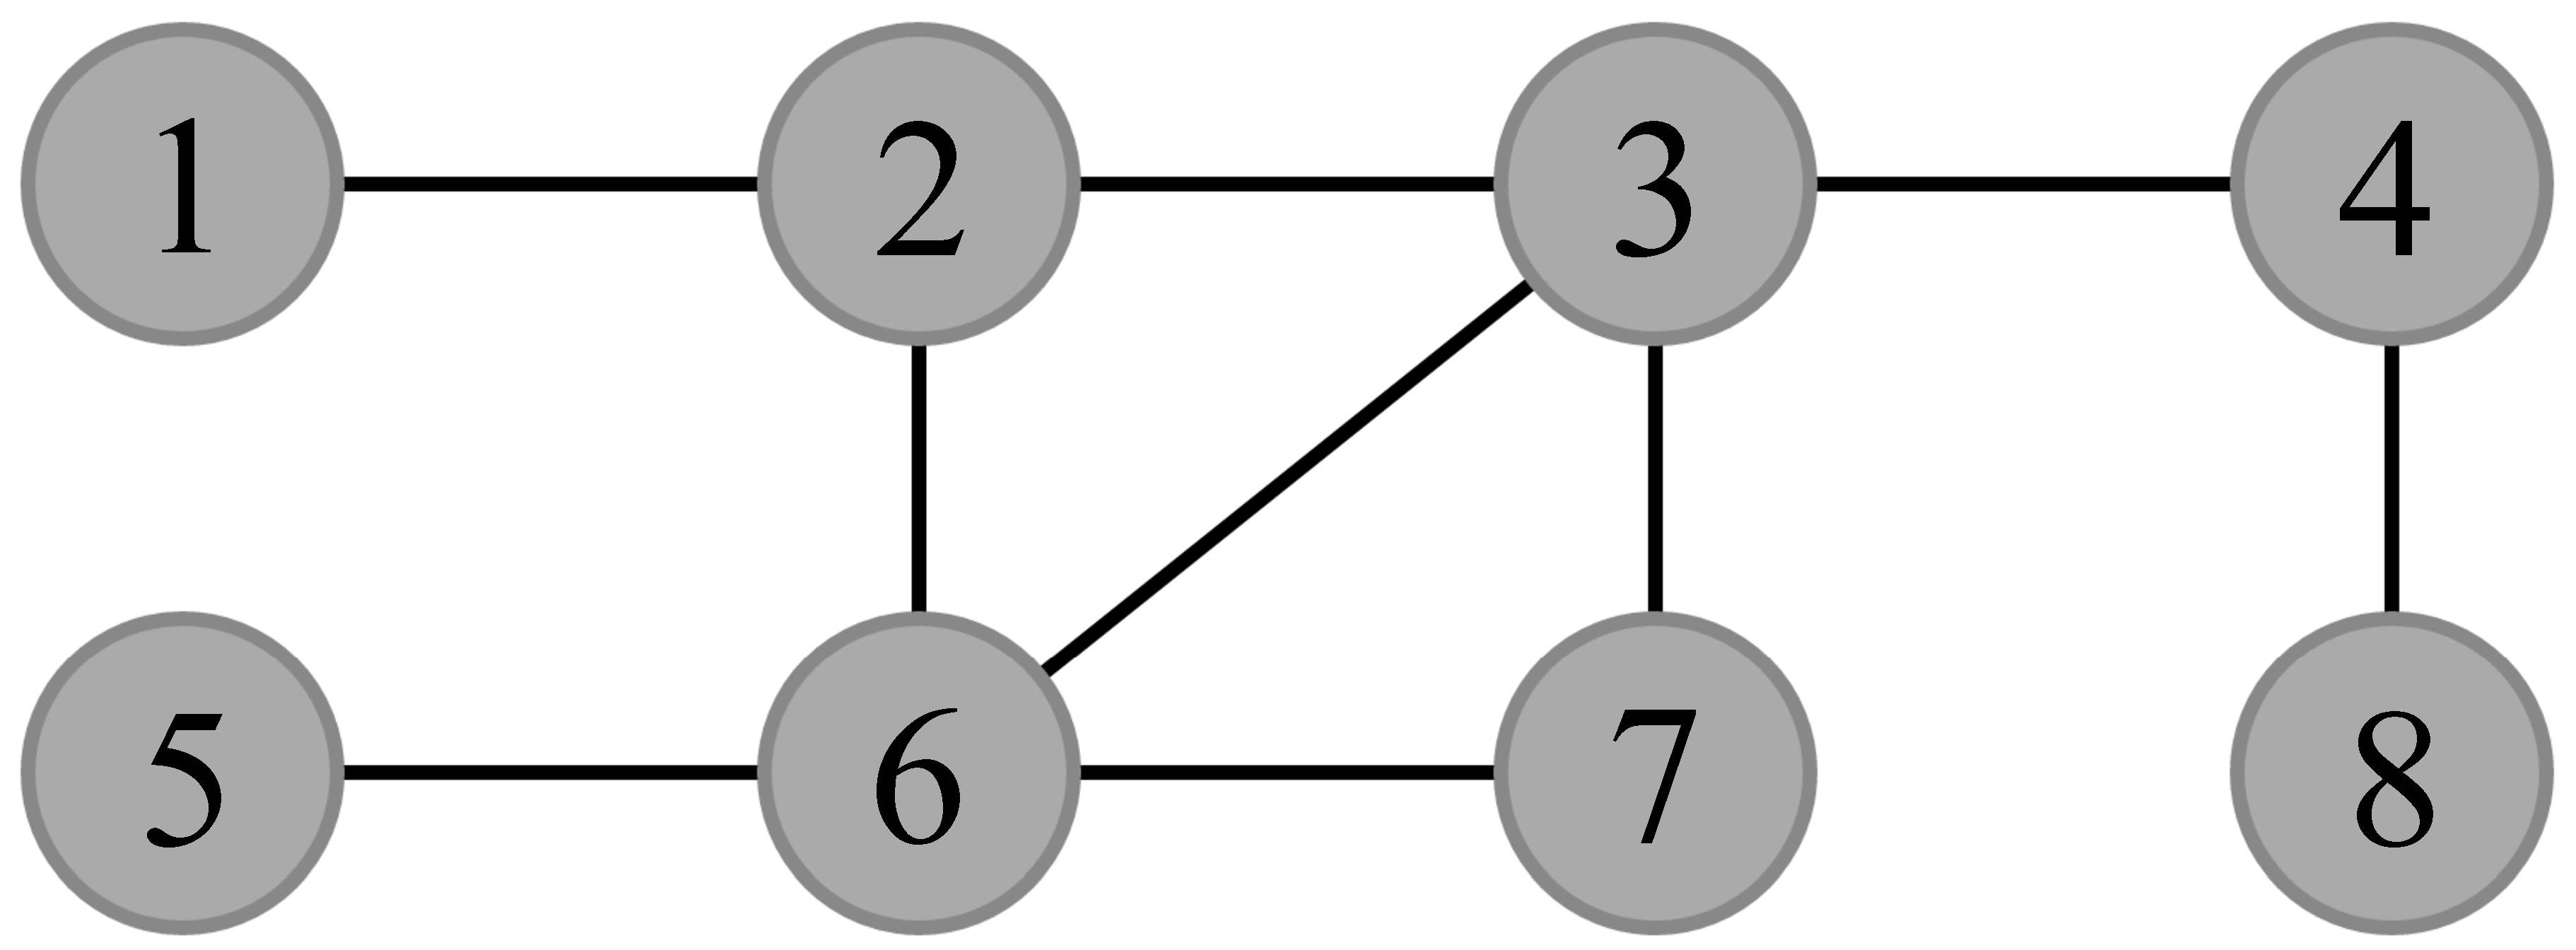
\includegraphics[width=5.7cm]{../figures/algorithm1.pdf}
            \caption*{A simple graph $G$}
          \end{figure}
        \end{textblock*}
      \end{center}
    \end{column}
  \end{columns}
}

\only<4>{
  \begin{textblock*}{8cm}(8cm, 8cm) % {block width} (coords)
    \begin{center}
      $D= \{8\}$
    \end{center}
  \end{textblock*}

  \begin{columns}
    \begin{column}{0.5\textwidth}
      \begin{algorithm}[H]
        \caption*{\textbf{Algorithm} IEDS}
        \scriptsize
        \begin{algorithmic}[1]
        \State $i \gets 1,\ P \gets \emptyset$
        \State Remove all isolated paths from $G$
        \While{$G$ is not empty}
          \State $D \gets \emptyset$
          \ForAll{components of $G$}
            \CSTATE Pick any vertex $v$
            \CSTATE $D \gets D \cup \{ v \}$
            \While{$\exists u$ at distance $\geq 3$ $\forall v \in D$}
              \State Pick $u$ at distance 3 from some vertex in $D$
              \State $D \gets D \cup \{ w \}$
            \EndWhile
            \ForAll{$u \in D$}
              \State Color $u$ with color $i$
            \EndFor
            \State $i \gets i + 1$
            \ForAll{$u \in D$}
              \State Remove $N(u)$ from $G$
            \EndFor
            \State Remove all isolated paths from G
          \EndFor
        \EndWhile
        \State Color all removed isolated paths using color $i$
        \end{algorithmic}
      \end{algorithm}
    \end{column}
    \begin{column}{0.5\textwidth}
      \begin{center}
        \begin{textblock*}{8cm}(8cm, 1.2cm) % {block width} (coords)
          \begin{figure}
            \centering
            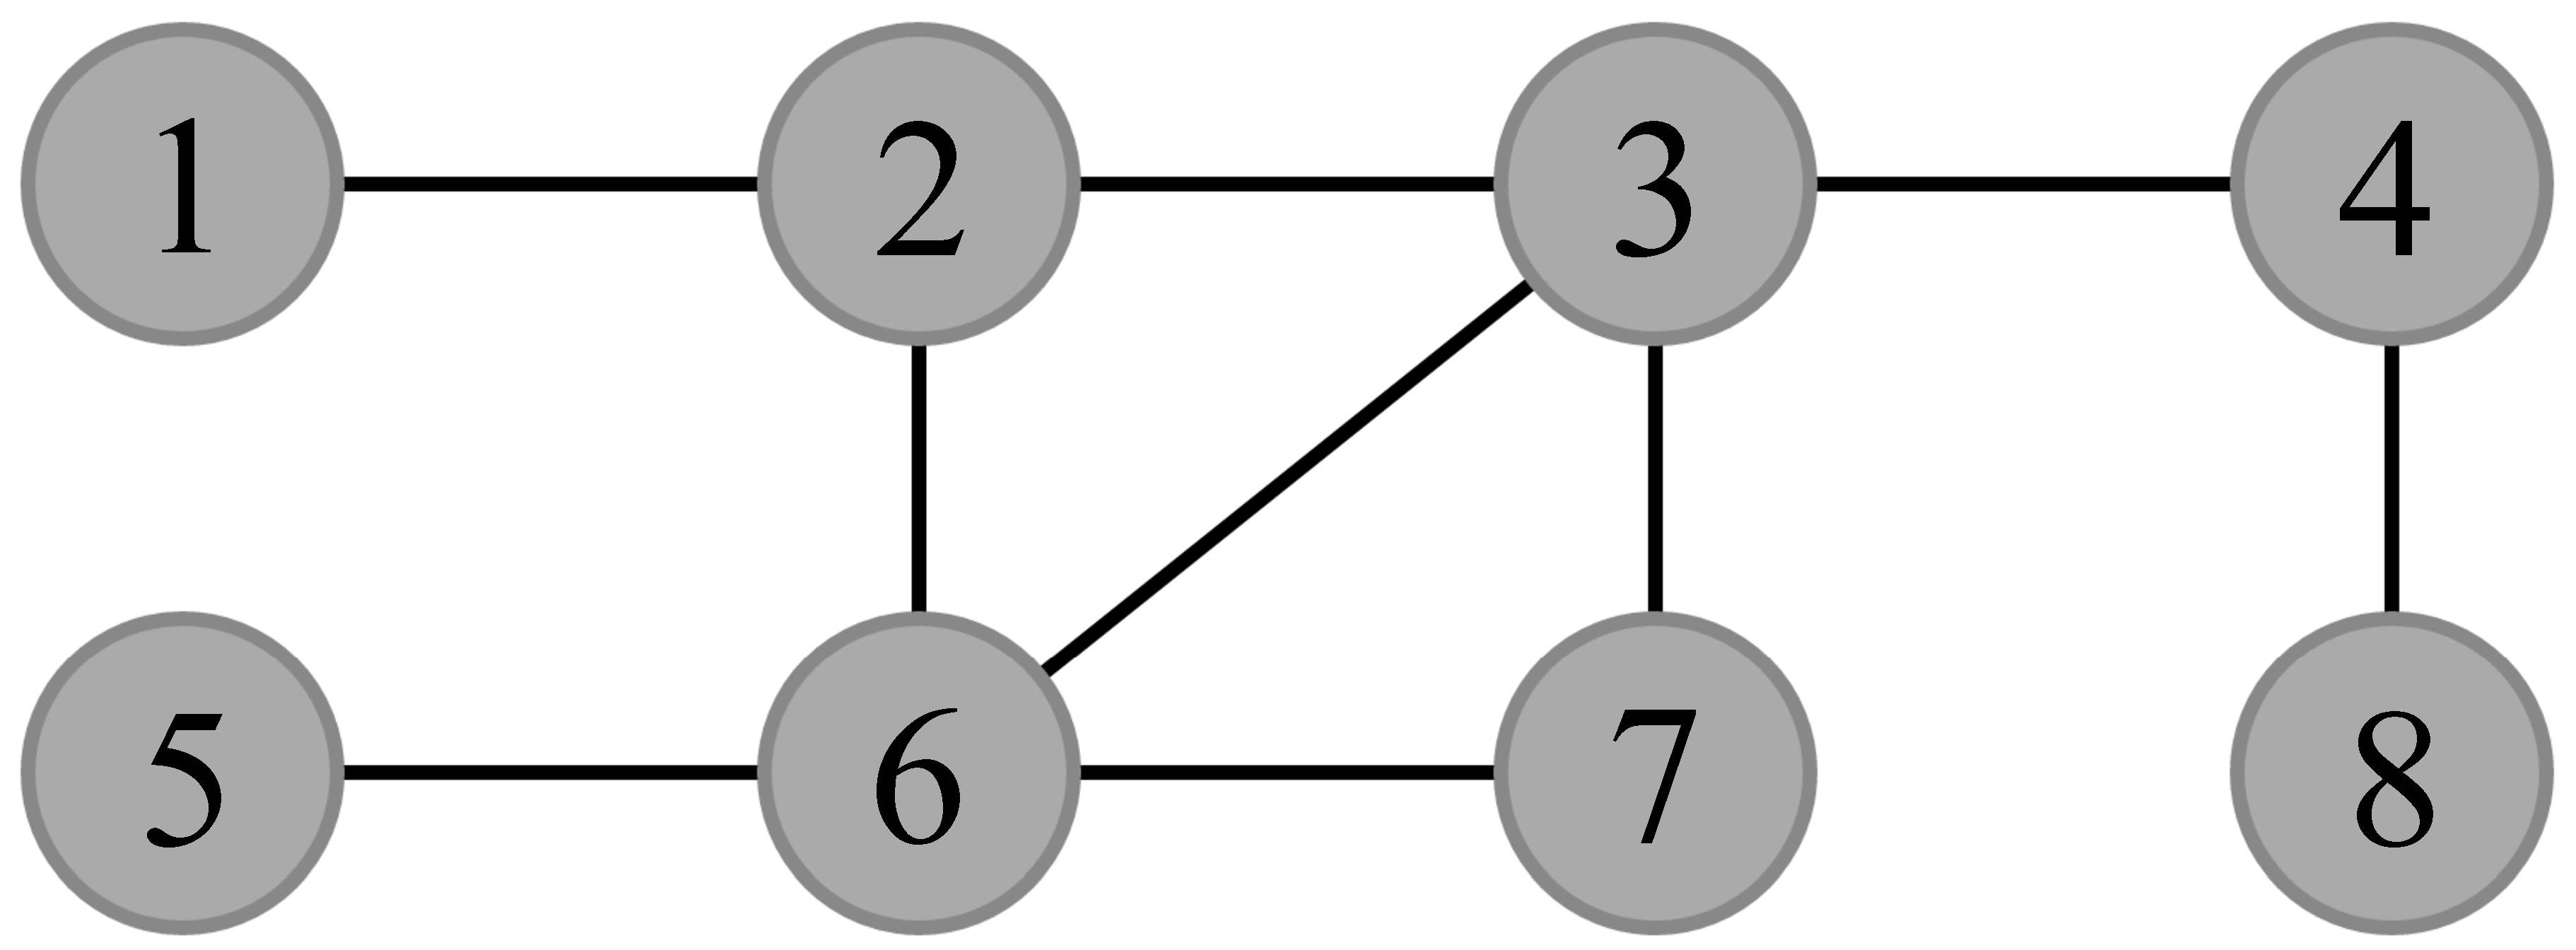
\includegraphics[width=5.7cm]{../figures/algorithm1.pdf}
            \caption*{Coloring of $G$ so far}
          \end{figure}
        \end{textblock*}
        \begin{textblock*}{8cm}(8cm, 4cm) % {block width} (coords)
          \begin{figure}
            \centering
            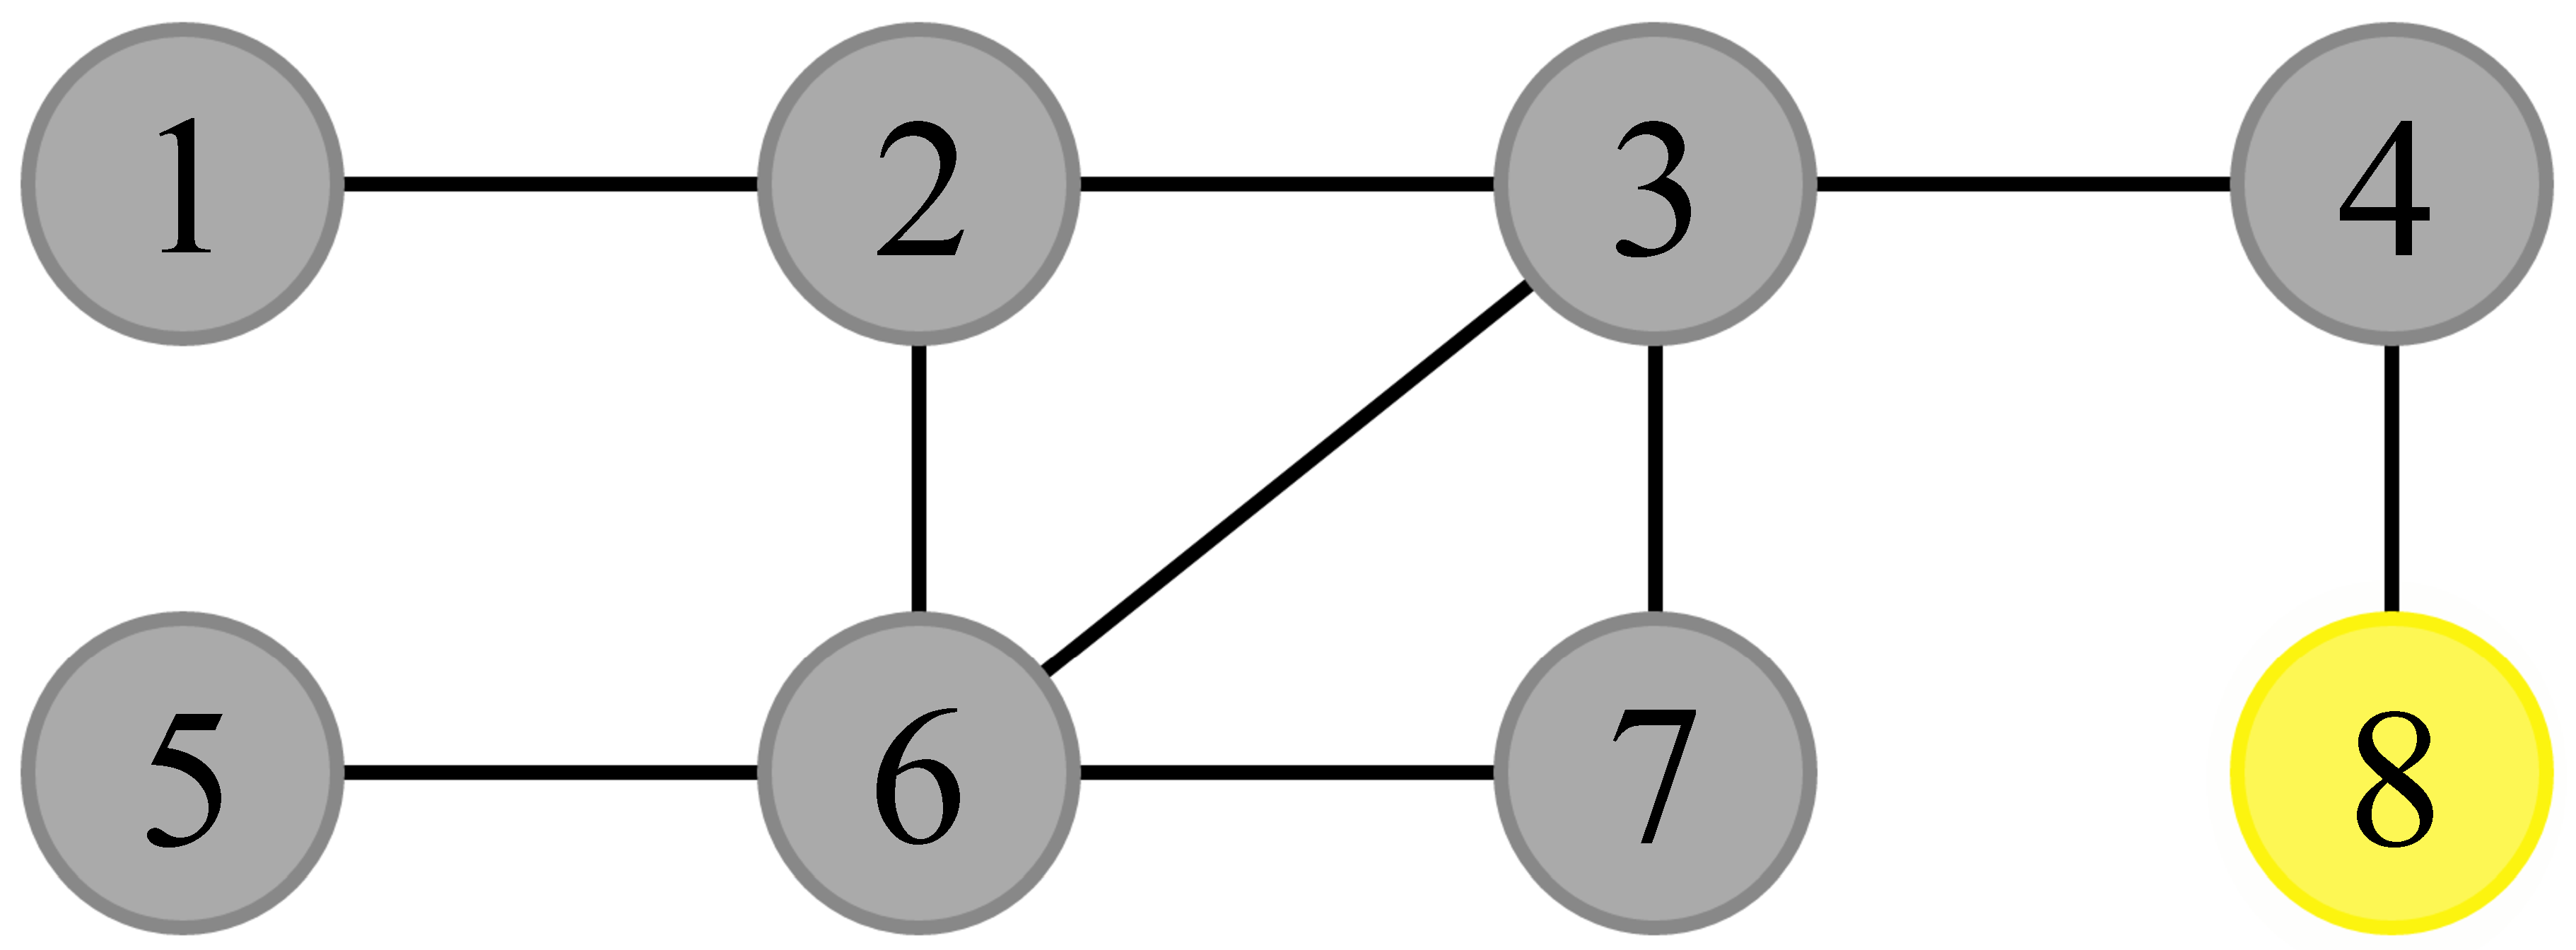
\includegraphics[width=5.7cm]{../figures/algorithm1-slide-1.pdf}
            \caption*{A simple graph $G$}
          \end{figure}
        \end{textblock*}
      \end{center}
    \end{column}
  \end{columns}
}

\only<5>{
  \begin{textblock*}{8cm}(8cm, 8cm) % {block width} (coords)
    \begin{center}
      $D= \{8\}$
    \end{center}
  \end{textblock*}

  \begin{columns}
    \begin{column}{0.5\textwidth}
      \begin{algorithm}[H]
        \caption*{\textbf{Algorithm} IEDS}
        \scriptsize
        \begin{algorithmic}[1]
        \State $i \gets 1,\ P \gets \emptyset$
        \State Remove all isolated paths from $G$
        \While{$G$ is not empty}
          \State $D \gets \emptyset$
          \ForAll{components of $G$}
            \State Pick any vertex $v$
            \State $D \gets D \cup \{ v \}$
            \CWhile{$\exists u$ at distance $\geq 3$ $\forall v \in D$}
              \State Pick $u$ at distance 3 from some vertex in $D$
              \State $D \gets D \cup \{ w \}$
            \EndWhile
            \ForAll{$u \in D$}
              \State Color $u$ with color $i$
            \EndFor
            \State $i \gets i + 1$
            \ForAll{$u \in D$}
              \State Remove $N(u)$ from $G$
            \EndFor
            \State Remove all isolated paths from G
          \EndFor
        \EndWhile
        \State Color all removed isolated paths using color $i$
        \end{algorithmic}
      \end{algorithm}
    \end{column}
    \begin{column}{0.5\textwidth}
      \begin{center}
        \begin{textblock*}{8cm}(8cm, 1.2cm) % {block width} (coords)
          \begin{figure}
            \centering
            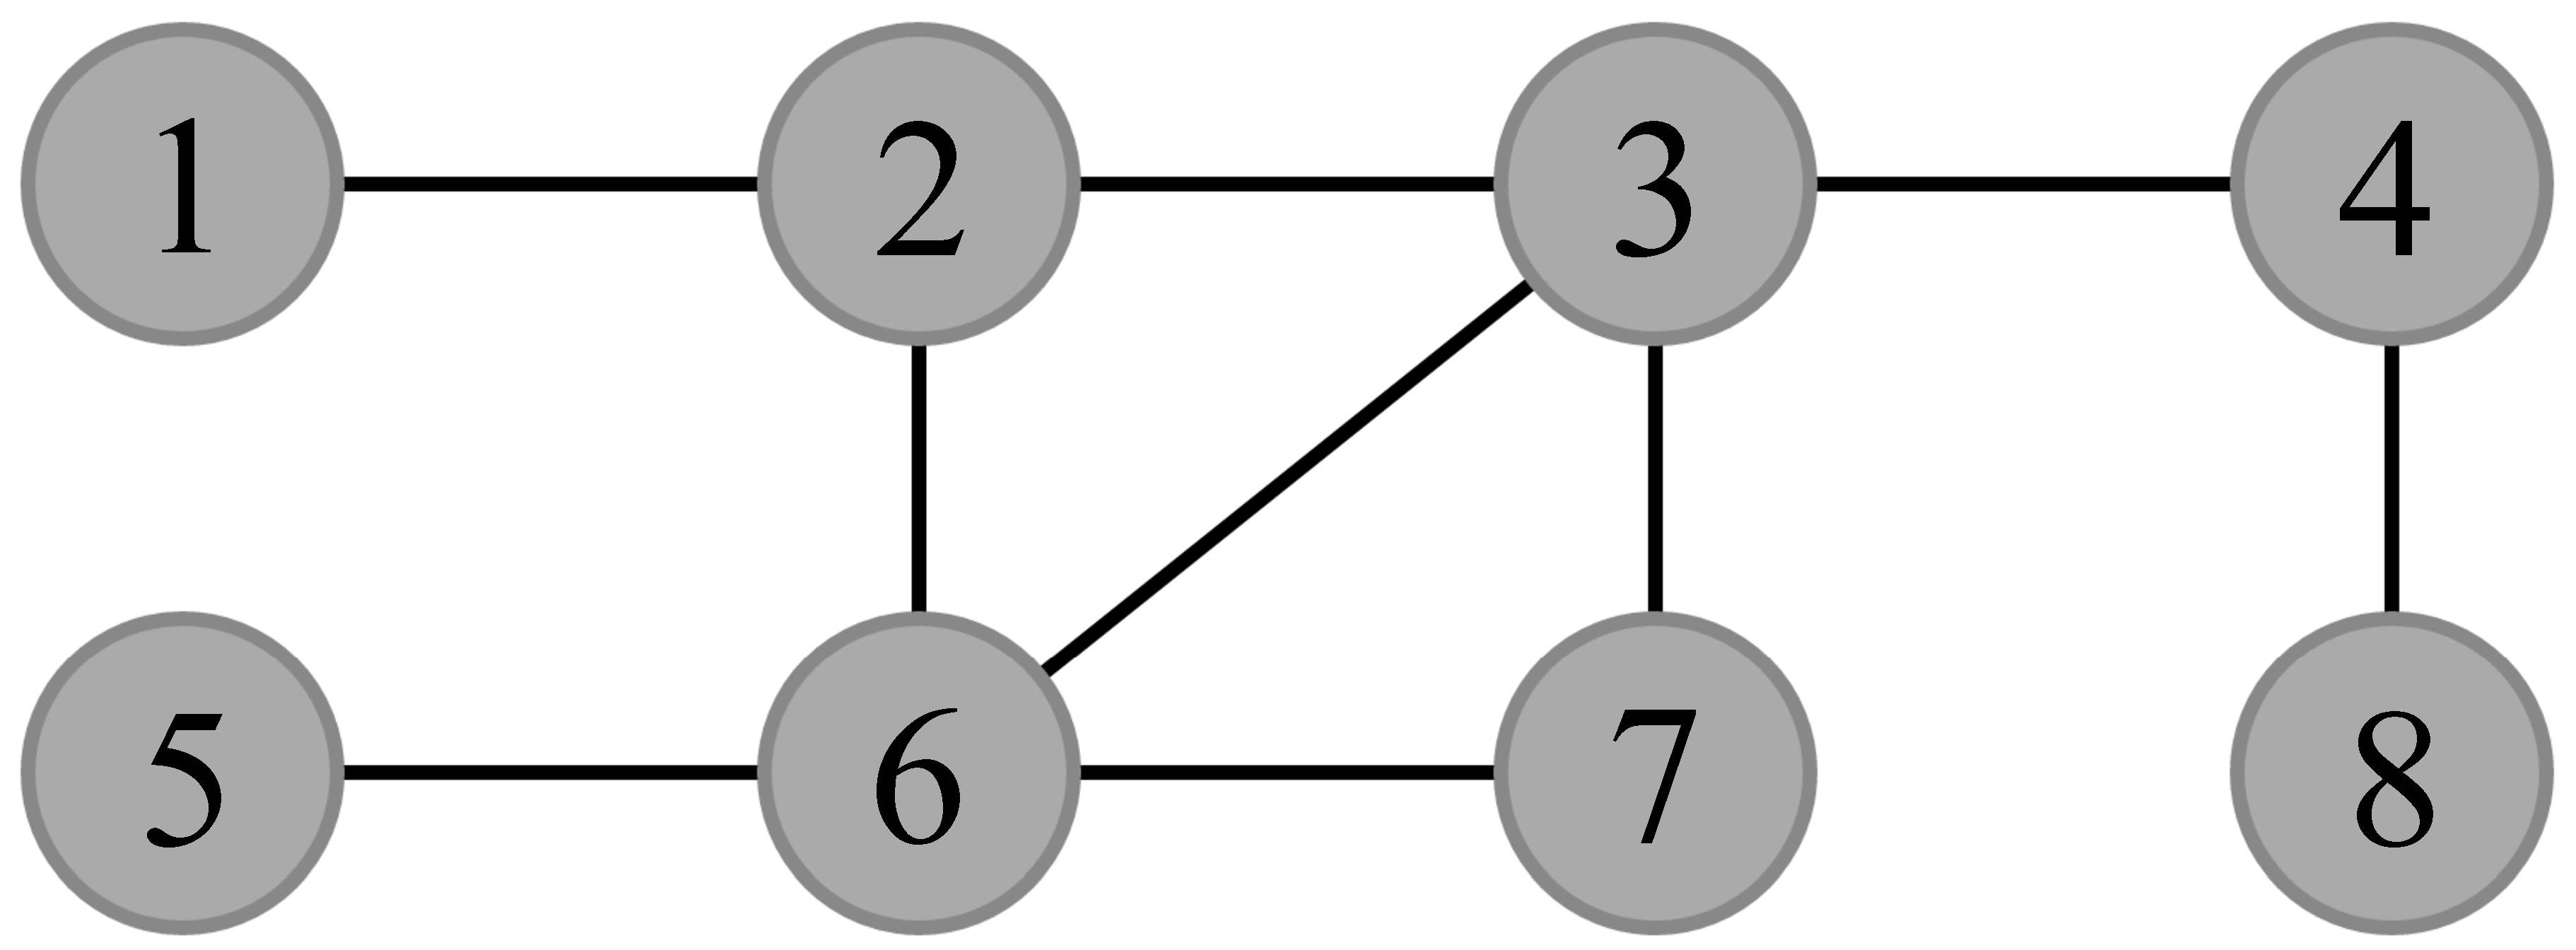
\includegraphics[width=5.7cm]{../figures/algorithm1.pdf}
            \caption*{Coloring of $G$ so far}
          \end{figure}
        \end{textblock*}
        \begin{textblock*}{8cm}(8cm, 4cm) % {block width} (coords)
          \begin{figure}
            \centering
            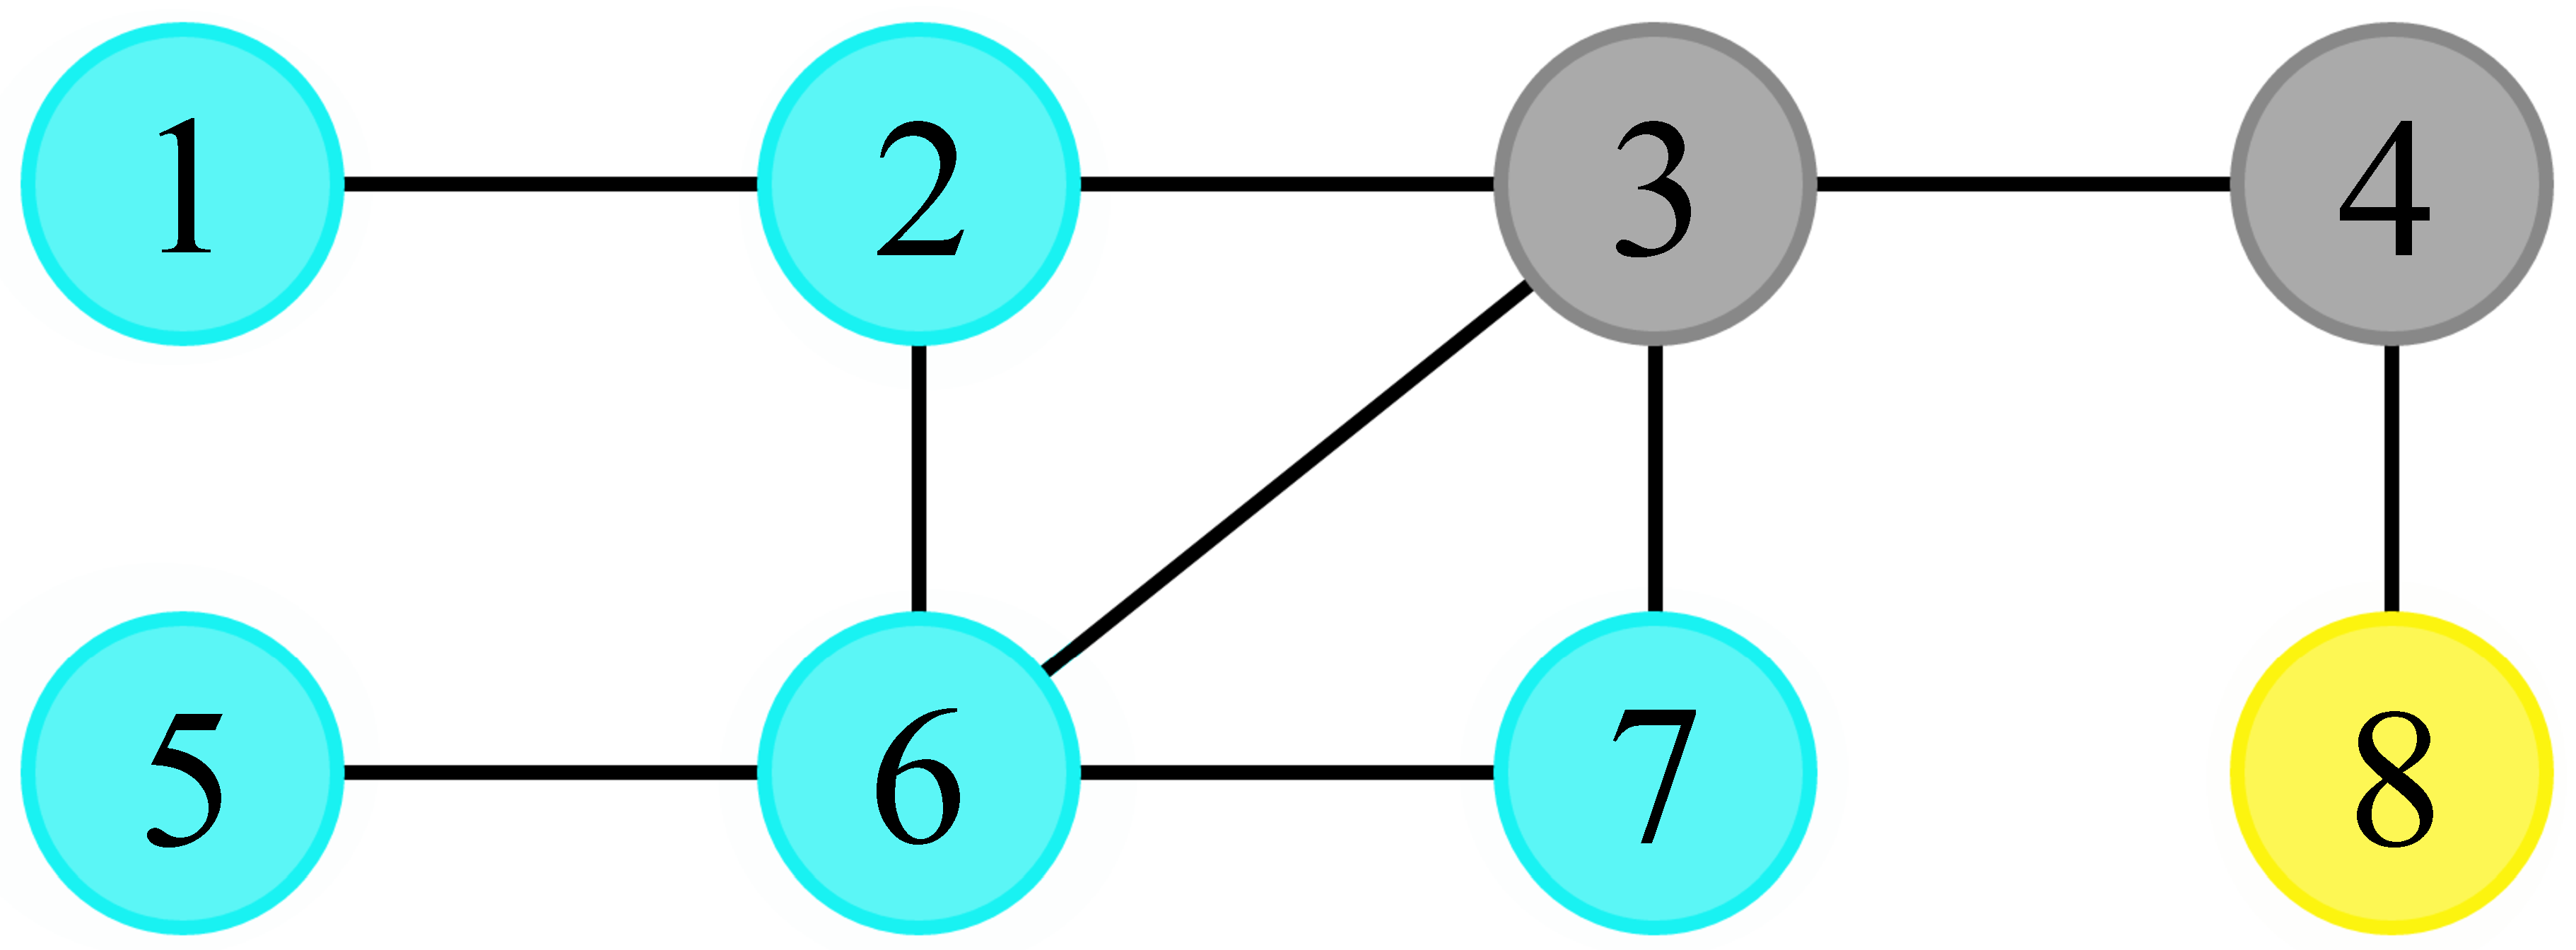
\includegraphics[width=5.7cm]{../figures/algorithm1-slide-25.pdf}
            \caption*{A simple graph $G$}
          \end{figure}
        \end{textblock*}
      \end{center}
    \end{column}
  \end{columns}
}

\only<6>{
  \begin{textblock*}{8cm}(8cm, 8cm) % {block width} (coords)
    \begin{center}
      $D= \{8\}$
    \end{center}
  \end{textblock*}

  \begin{columns}
    \begin{column}{0.5\textwidth}
      \begin{algorithm}[H]
        \caption*{\textbf{Algorithm} IEDS}
        \scriptsize
        \begin{algorithmic}[1]
        \State $i \gets 1,\ P \gets \emptyset$
        \State Remove all isolated paths from $G$
        \While{$G$ is not empty}
          \State $D \gets \emptyset$
          \ForAll{components of $G$}
            \State Pick any vertex $v$
            \State $D \gets D \cup \{ v \}$
            \While{$\exists u$ at distance $\geq 3$ $\forall v \in D$}
              \CSTATE Pick $u$ at distance 3 from some vertex in $D$
              \State $D \gets D \cup \{ w \}$
            \EndWhile
            \ForAll{$u \in D$}
              \State Color $u$ with color $i$
            \EndFor
            \State $i \gets i + 1$
            \ForAll{$u \in D$}
              \State Remove $N(u)$ from $G$
            \EndFor
            \State Remove all isolated paths from G
          \EndFor
        \EndWhile
        \State Color all removed isolated paths using color $i$
        \end{algorithmic}
      \end{algorithm}
    \end{column}
    \begin{column}{0.5\textwidth}
      \begin{center}
        \begin{textblock*}{8cm}(8cm, 1.2cm) % {block width} (coords)
          \begin{figure}
            \centering
            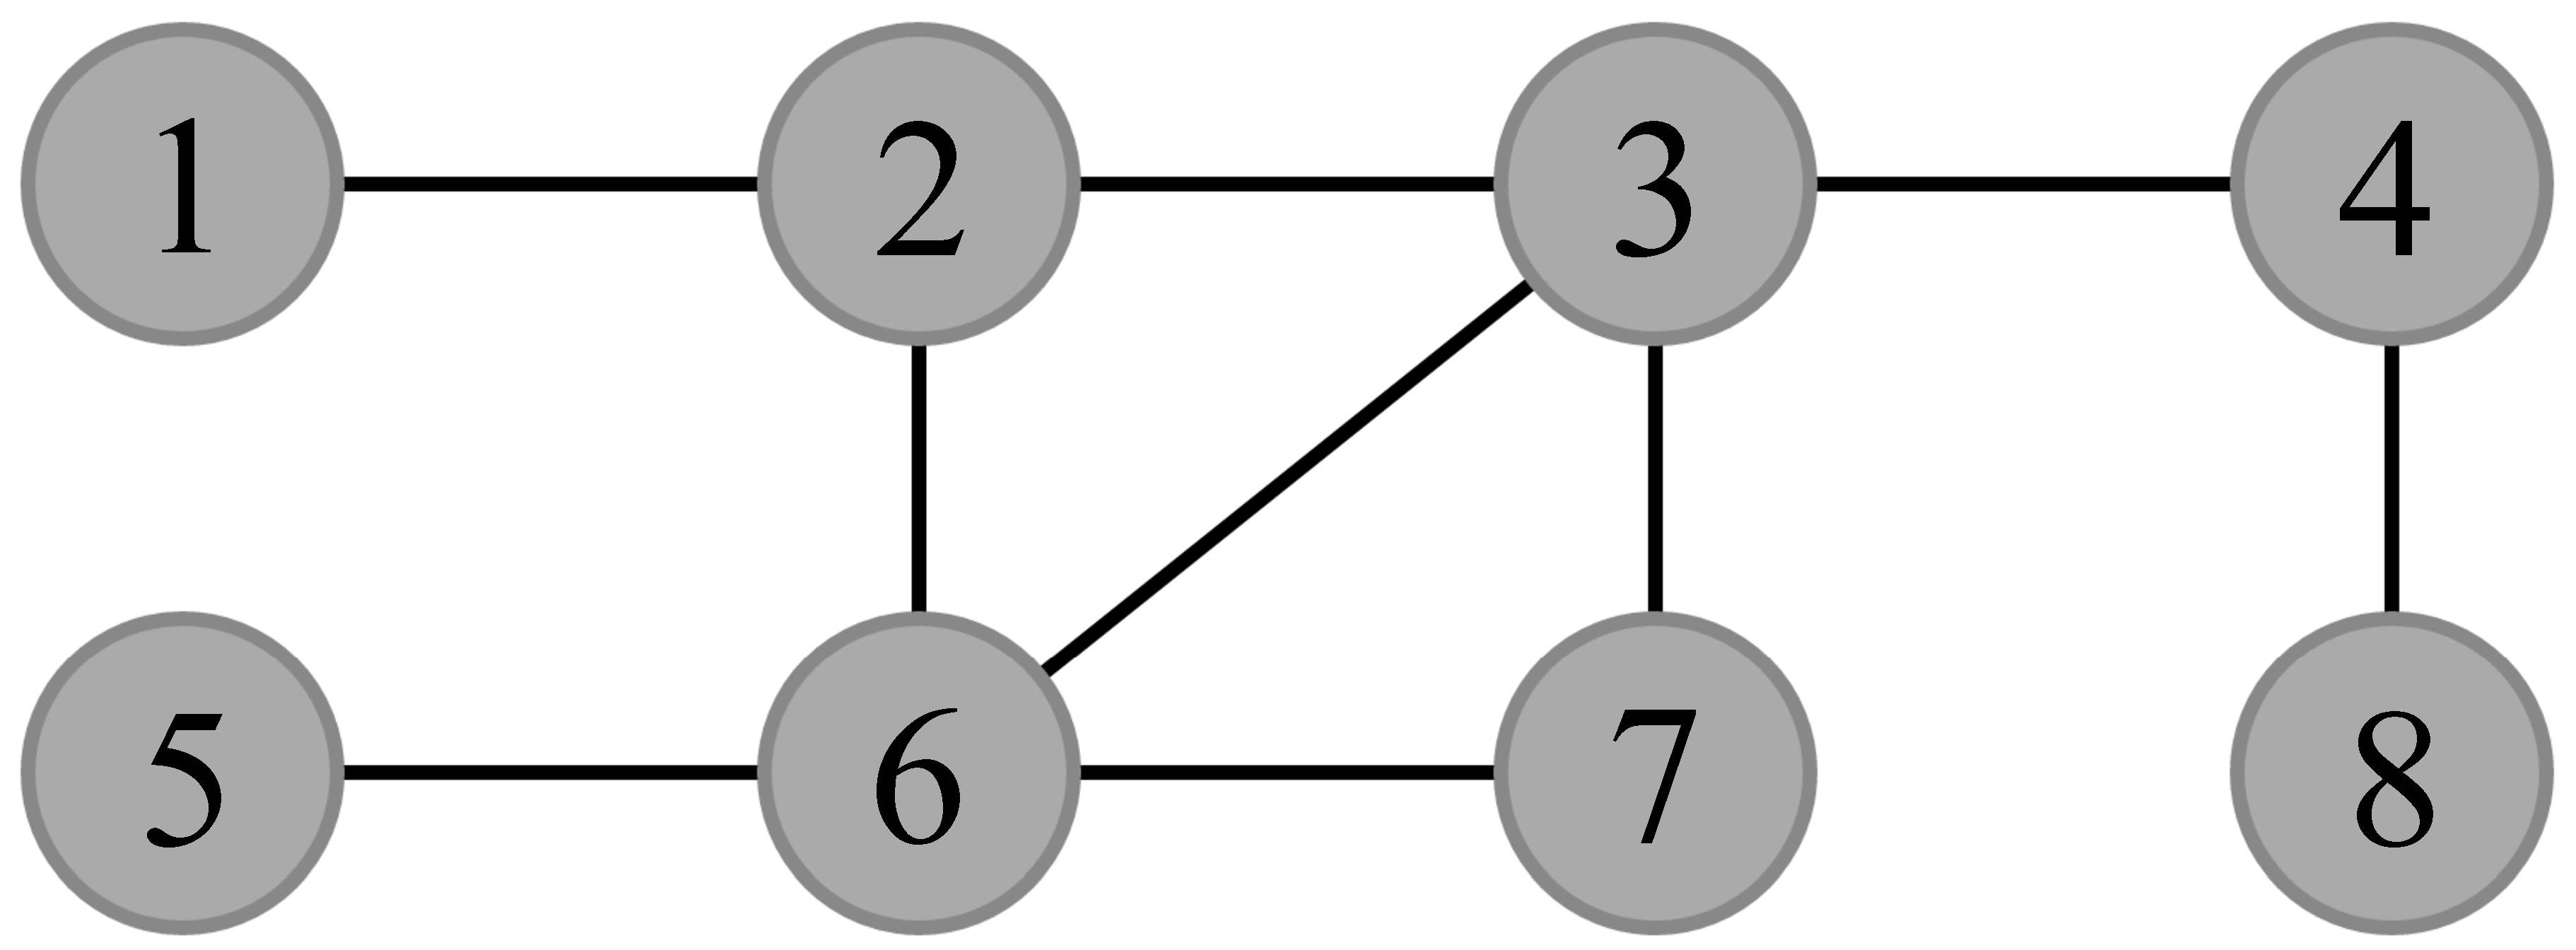
\includegraphics[width=5.7cm]{../figures/algorithm1.pdf}
            \caption*{Coloring of $G$ so far}
          \end{figure}
        \end{textblock*}
        \begin{textblock*}{8cm}(8cm, 4cm) % {block width} (coords)
          \begin{figure}
            \centering
            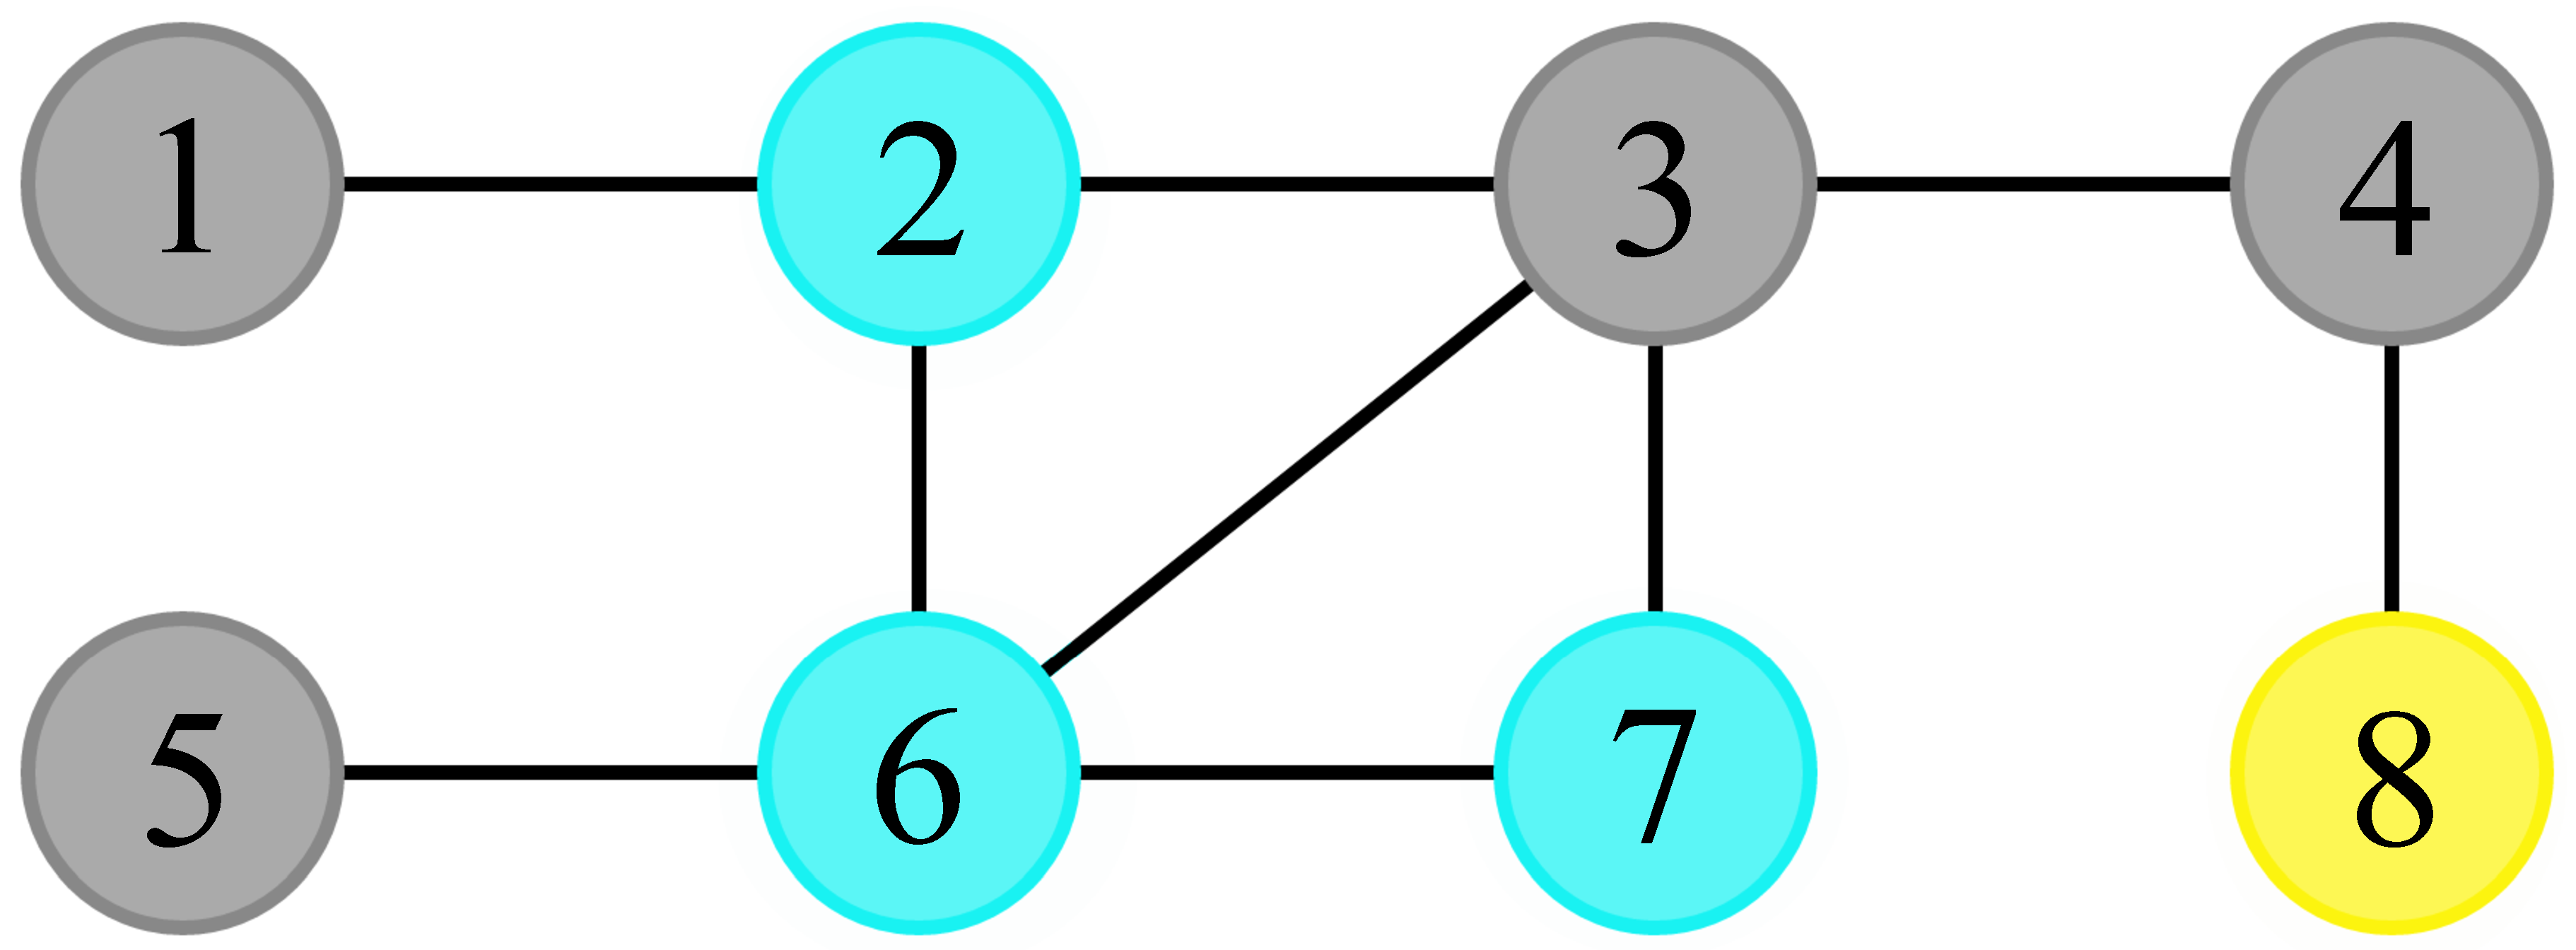
\includegraphics[width=5.7cm]{../figures/algorithm1-slide-2.pdf}
            \caption*{A simple graph $G$}
          \end{figure}
        \end{textblock*}
      \end{center}
    \end{column}
  \end{columns}
}

\only<7>{
  \begin{textblock*}{8cm}(8cm, 8cm) % {block width} (coords)
    \begin{center}
      $D= \{2,8\}$
    \end{center}
  \end{textblock*}

  \begin{columns}
    \begin{column}{0.5\textwidth}
      \begin{algorithm}[H]
        \caption*{\textbf{Algorithm} IEDS}
        \scriptsize
        \begin{algorithmic}[1]
        \State $i \gets 1,\ P \gets \emptyset$
        \State Remove all isolated paths from $G$
        \While{$G$ is not empty}
          \State $D \gets \emptyset$
          \ForAll{components of $G$}
            \State Pick any vertex $v$
            \State $D \gets D \cup \{ v \}$
            \While{$\exists u$ at distance $\geq 3$ $\forall v \in D$}
              \State Pick $u$ at distance 3 from some vertex in $D$
              \CSTATE $D \gets D \cup \{ w \}$
            \EndWhile
            \ForAll{$u \in D$}
              \State Color $u$ with color $i$
            \EndFor
            \State $i \gets i + 1$
            \ForAll{$u \in D$}
              \State Remove $N(u)$ from $G$
            \EndFor
            \State Remove all isolated paths from G
          \EndFor
        \EndWhile
        \State Color all removed isolated paths using color $i$
        \end{algorithmic}
      \end{algorithm}
    \end{column}
    \begin{column}{0.5\textwidth}
      \begin{center}
        \begin{textblock*}{8cm}(8cm, 1.2cm) % {block width} (coords)
          \begin{figure}
            \centering
            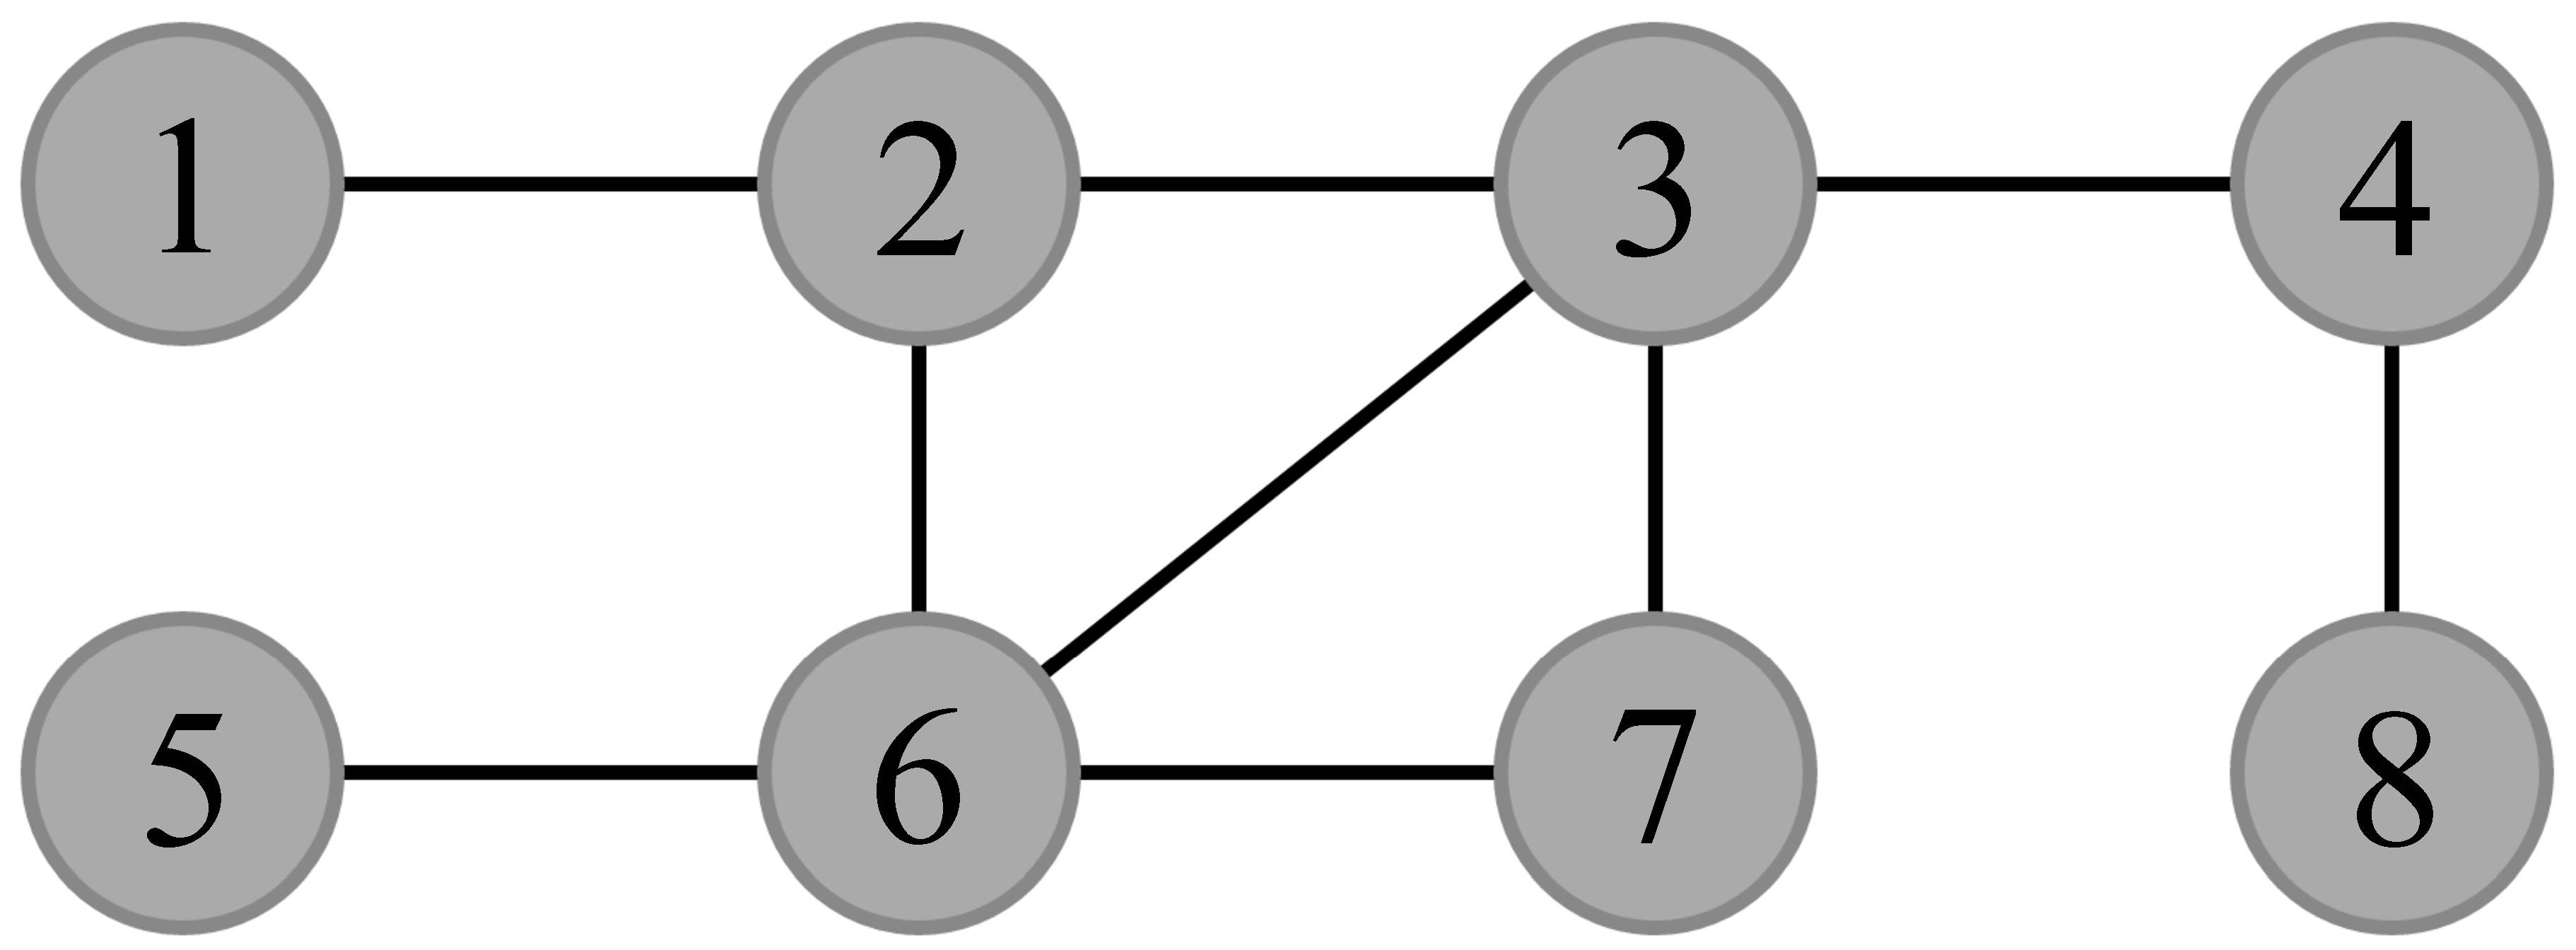
\includegraphics[width=5.7cm]{../figures/algorithm1.pdf}
            \caption*{Coloring of $G$ so far}
          \end{figure}
        \end{textblock*}
        \begin{textblock*}{8cm}(8cm, 4cm) % {block width} (coords)
          \begin{figure}
            \centering
            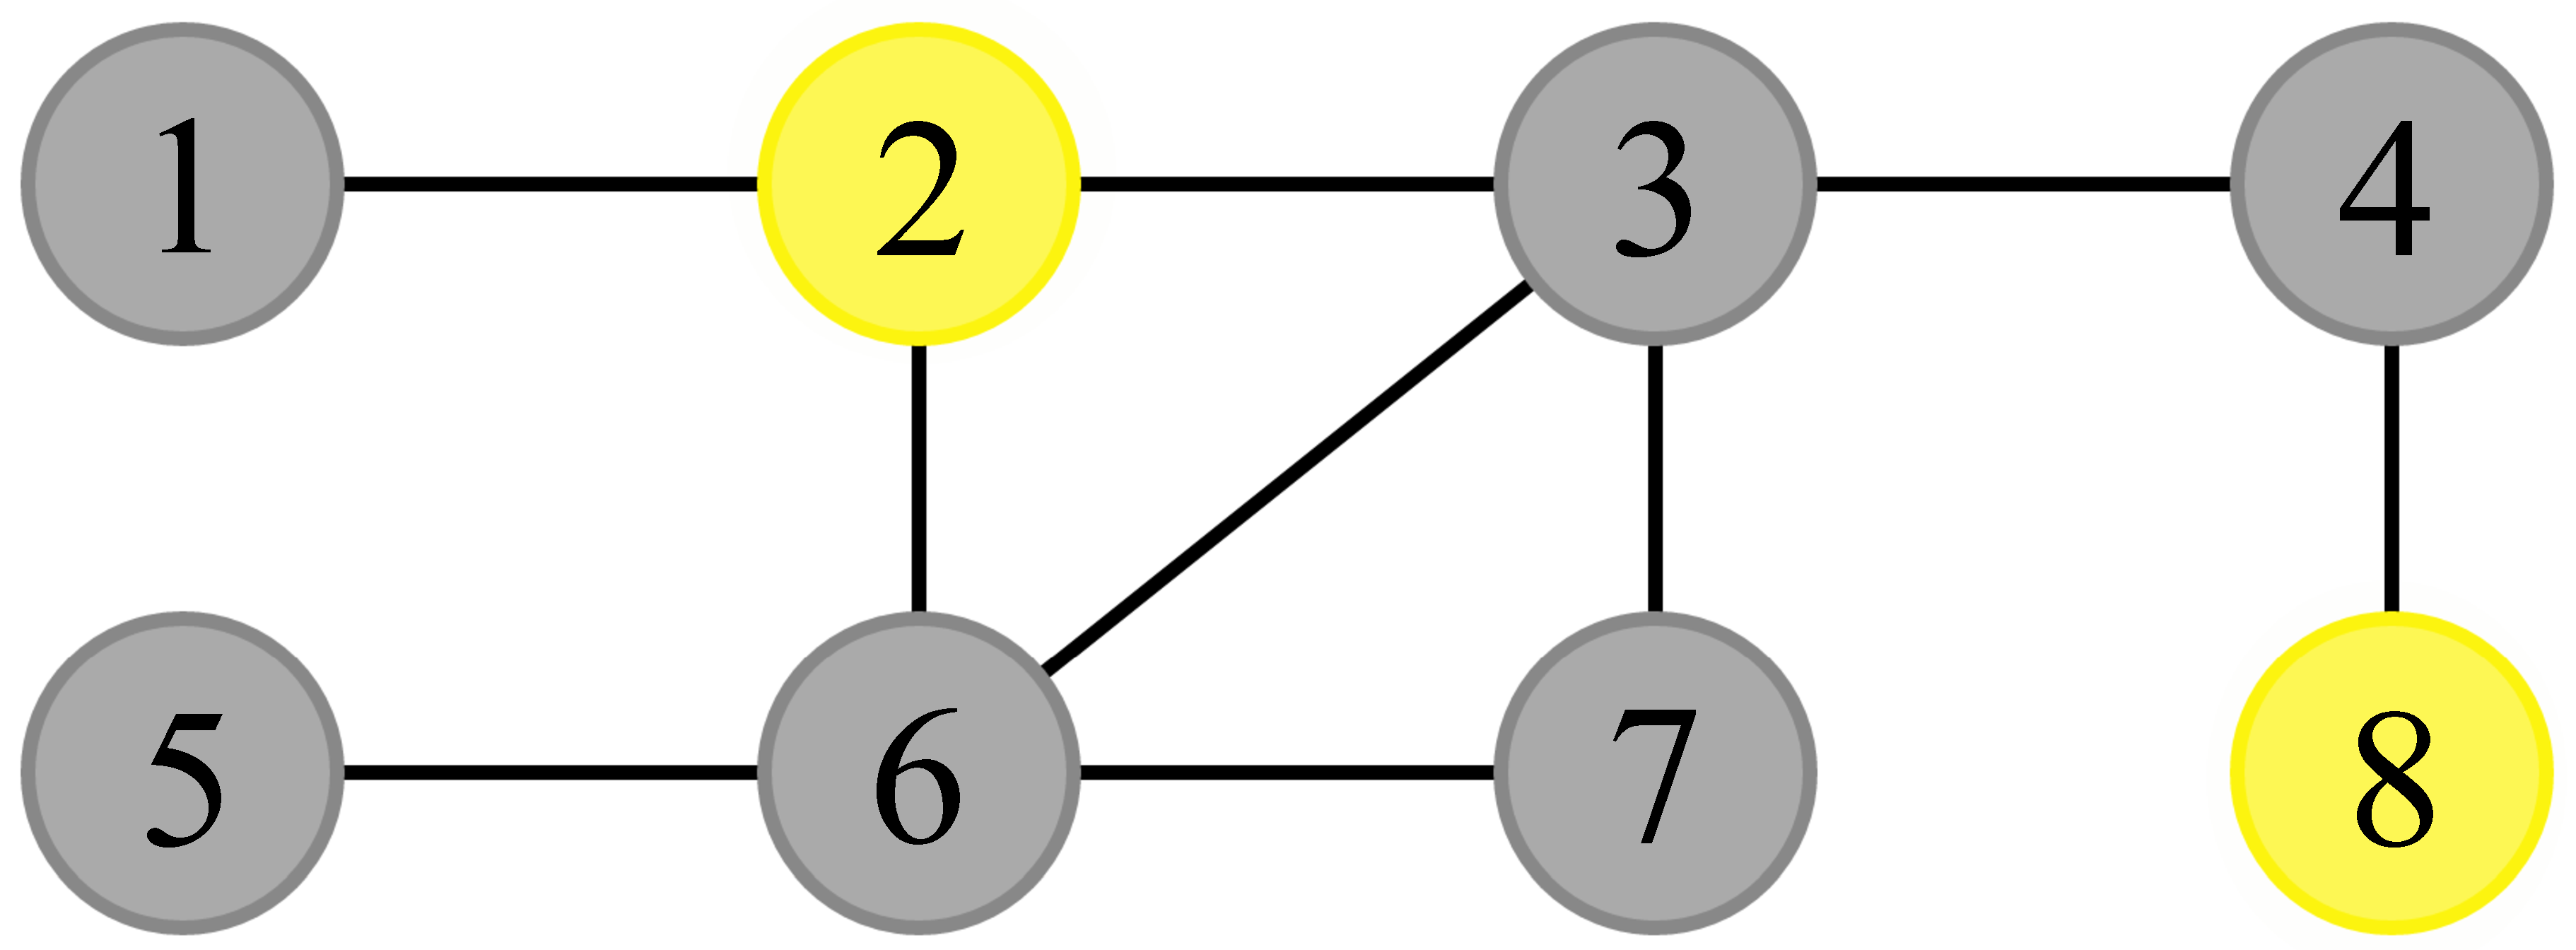
\includegraphics[width=5.7cm]{../figures/algorithm1-slide-3.pdf}
            \caption*{A simple graph $G$}
          \end{figure}
        \end{textblock*}
      \end{center}
    \end{column}
  \end{columns}
}

\only<8>{
  \begin{textblock*}{8cm}(8cm, 8cm) % {block width} (coords)
    \begin{center}
      $D= \{2,8\}$
    \end{center}
  \end{textblock*}

  \begin{columns}
    \begin{column}{0.5\textwidth}
      \begin{algorithm}[H]
        \caption*{\textbf{Algorithm} IEDS}
        \scriptsize
        \begin{algorithmic}[1]
        \State $i \gets 1,\ P \gets \emptyset$
        \State Remove all isolated paths from $G$
        \While{$G$ is not empty}
          \State $D \gets \emptyset$
          \ForAll{components of $G$}
            \State Pick any vertex $v$
            \State $D \gets D \cup \{ v \}$
            \CWhile{$\exists u$ at distance $\geq 3$ $\forall v \in D$}
              \State Pick $u$ at distance 3 from some vertex in $D$
              \State $D \gets D \cup \{ w \}$
            \EndWhile
            \ForAll{$u \in D$}
              \State Color $u$ with color $i$
            \EndFor
            \State $i \gets i + 1$
            \ForAll{$u \in D$}
              \State Remove $N(u)$ from $G$
            \EndFor
            \State Remove all isolated paths from G
          \EndFor
        \EndWhile
        \State Color all removed isolated paths using color $i$
        \end{algorithmic}
      \end{algorithm}
    \end{column}
    \begin{column}{0.5\textwidth}
      \begin{center}
        \begin{textblock*}{8cm}(8cm, 1.2cm) % {block width} (coords)
          \begin{figure}
            \centering
            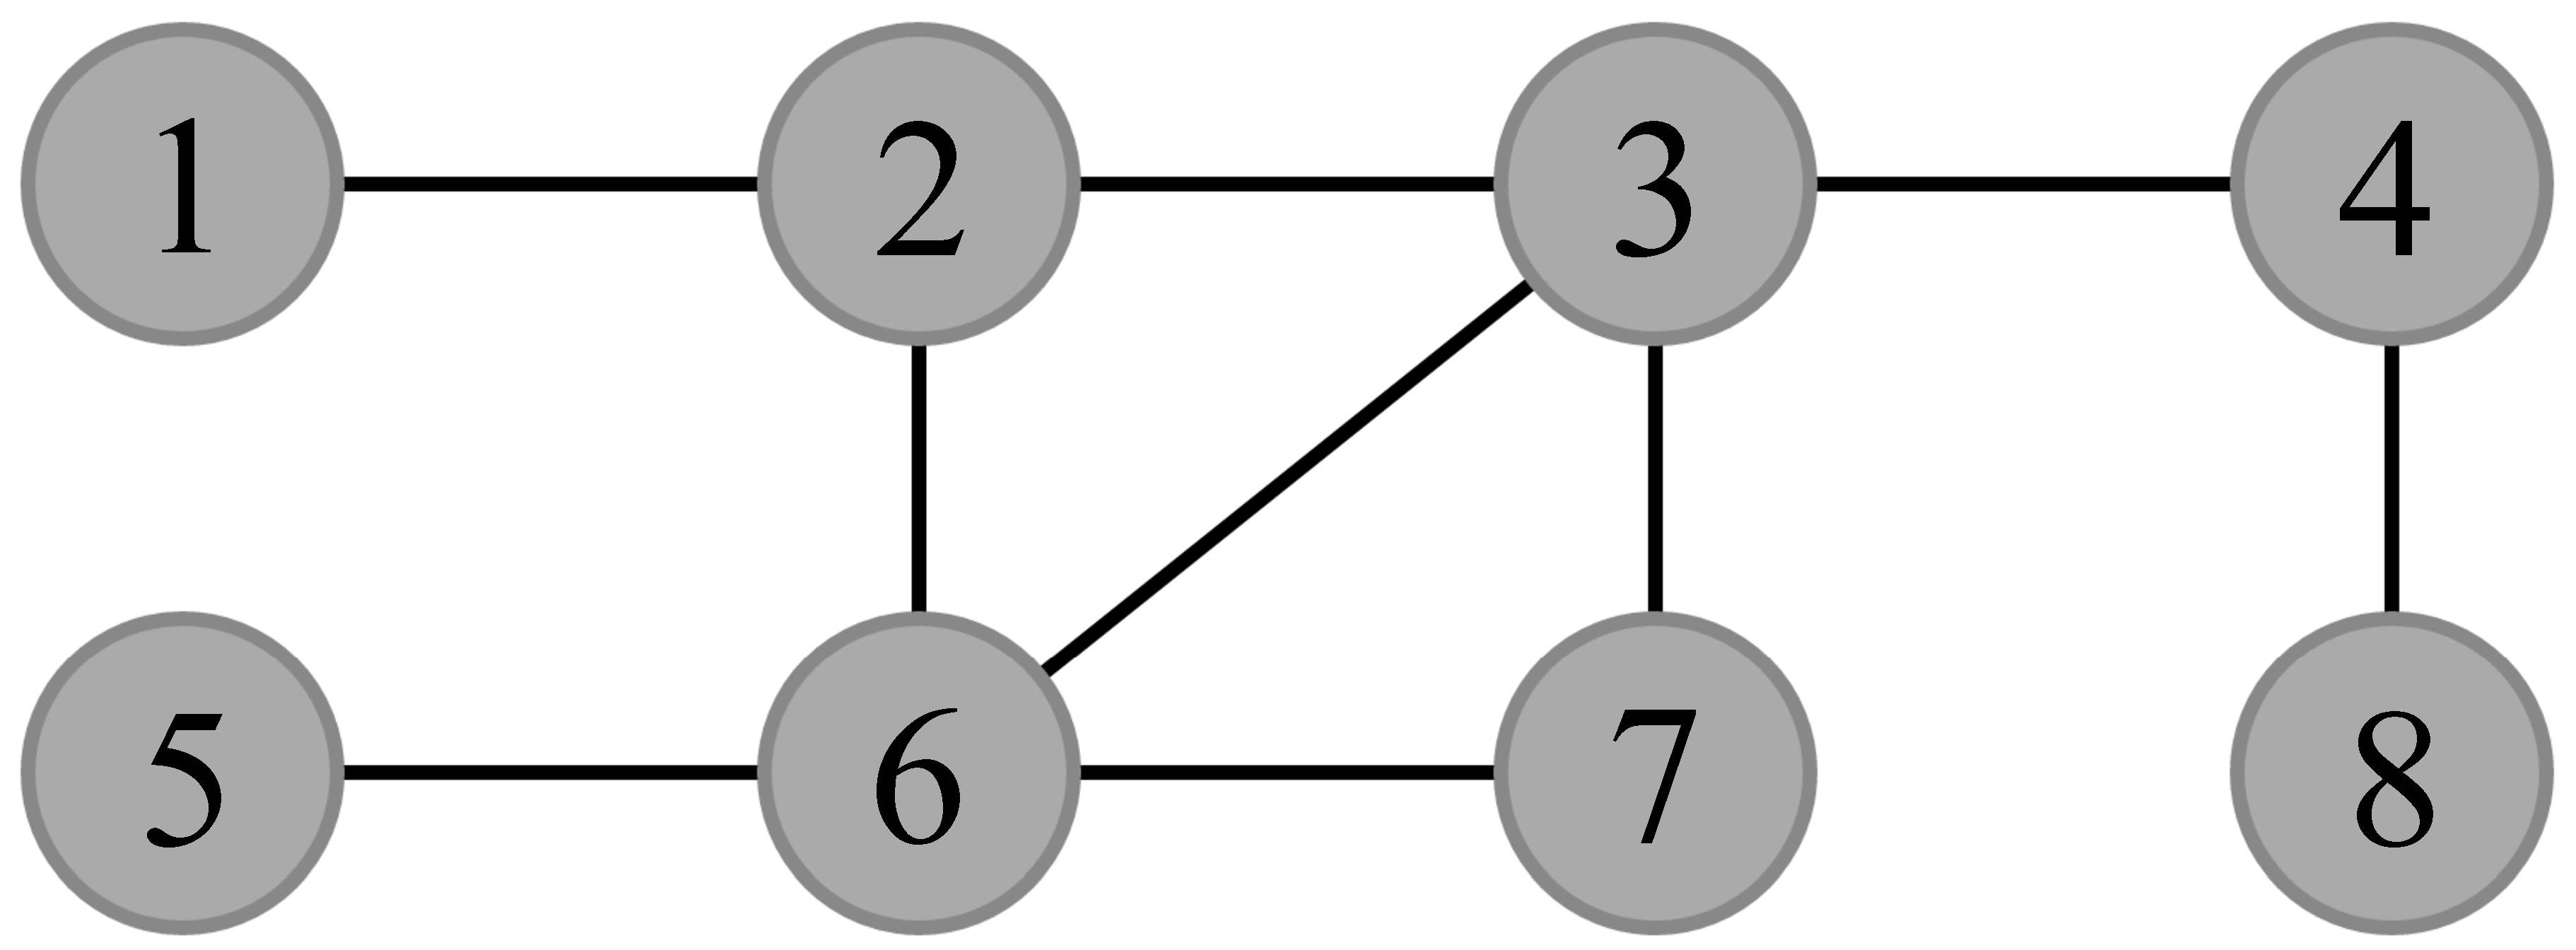
\includegraphics[width=5.7cm]{../figures/algorithm1.pdf}
            \caption*{Coloring of $G$ so far}
          \end{figure}
        \end{textblock*}
        \begin{textblock*}{8cm}(8cm, 4cm) % {block width} (coords)
          \begin{figure}
            \centering
            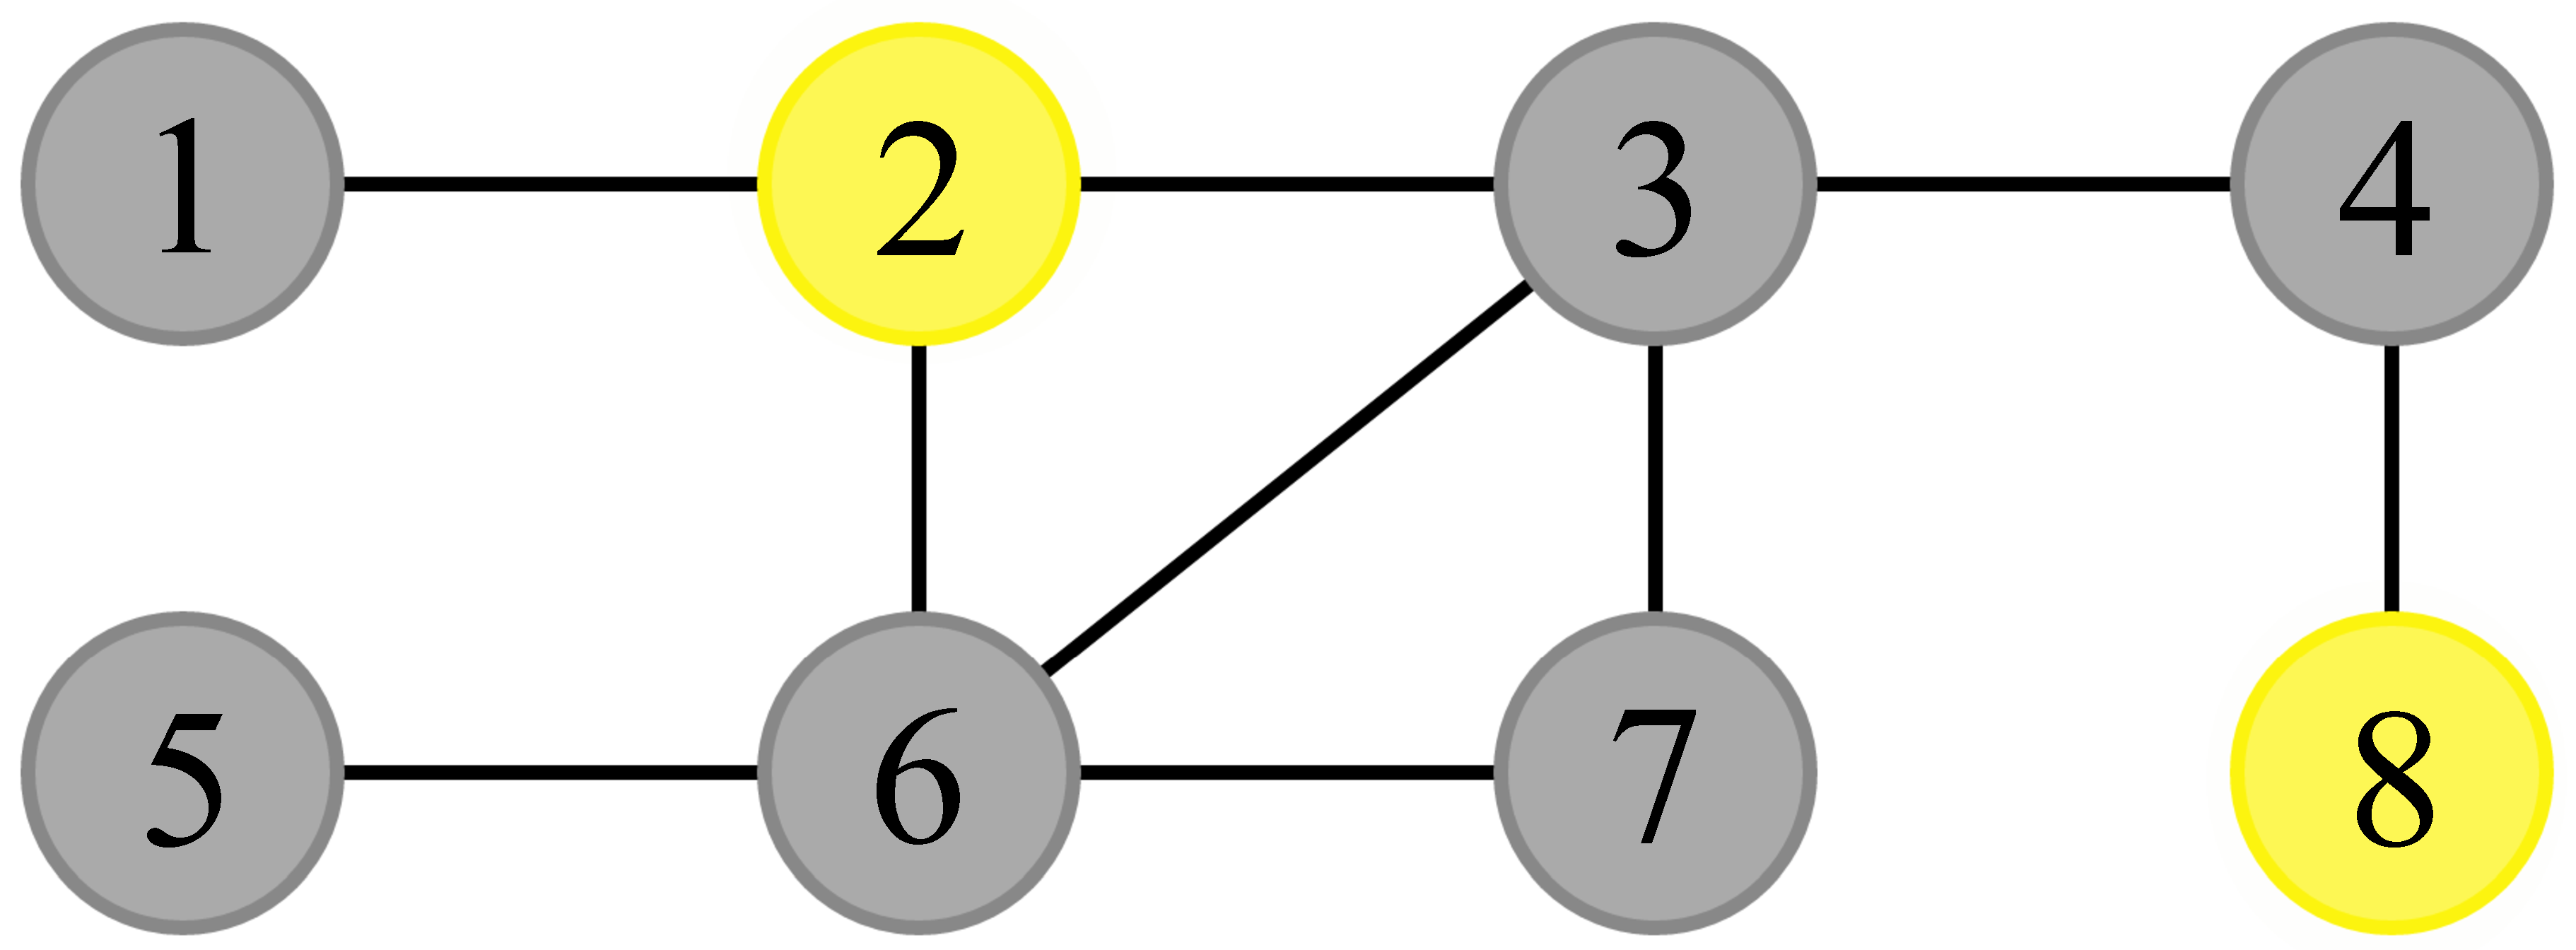
\includegraphics[width=5.7cm]{../figures/algorithm1-slide-3.pdf}
            \caption*{A simple graph $G$}
          \end{figure}
        \end{textblock*}
      \end{center}
    \end{column}
  \end{columns}
}

\only<9>{
  \begin{textblock*}{8cm}(8cm, 8cm) % {block width} (coords)
    \begin{center}
      $D= \{2,8\}$
    \end{center}
  \end{textblock*}

  \begin{columns}
    \begin{column}{0.5\textwidth}
      \begin{algorithm}[H]
        \caption*{\textbf{Algorithm} IEDS}
        \scriptsize
        \begin{algorithmic}[1]
        \State $i \gets 1,\ P \gets \emptyset$
        \State Remove all isolated paths from $G$
        \While{$G$ is not empty}
          \State $D \gets \emptyset$
          \ForAll{components of $G$}
            \State Pick any vertex $v$
            \State $D \gets D \cup \{ v \}$
            \While{$\exists u$ at distance $\geq 3$ $\forall v \in D$}
              \State Pick $u$ at distance 3 from some vertex in $D$
              \State $D \gets D \cup \{ w \}$
            \EndWhile
            \CForAll{$u \in D$}
              \CSTATE Color $u$ with color $i$
            \EndFor
            \CSTATE $i \gets i + 1$
            \ForAll{$u \in D$}
              \State Remove $N(u)$ from $G$
            \EndFor
            \State Remove all isolated paths from G
          \EndFor
        \EndWhile
        \State Color all removed isolated paths using color $i$
        \end{algorithmic}
      \end{algorithm}
    \end{column}
    \begin{column}{0.5\textwidth}
      \begin{center}
        \begin{textblock*}{8cm}(8cm, 1.2cm) % {block width} (coords)
          \begin{figure}
            \centering
            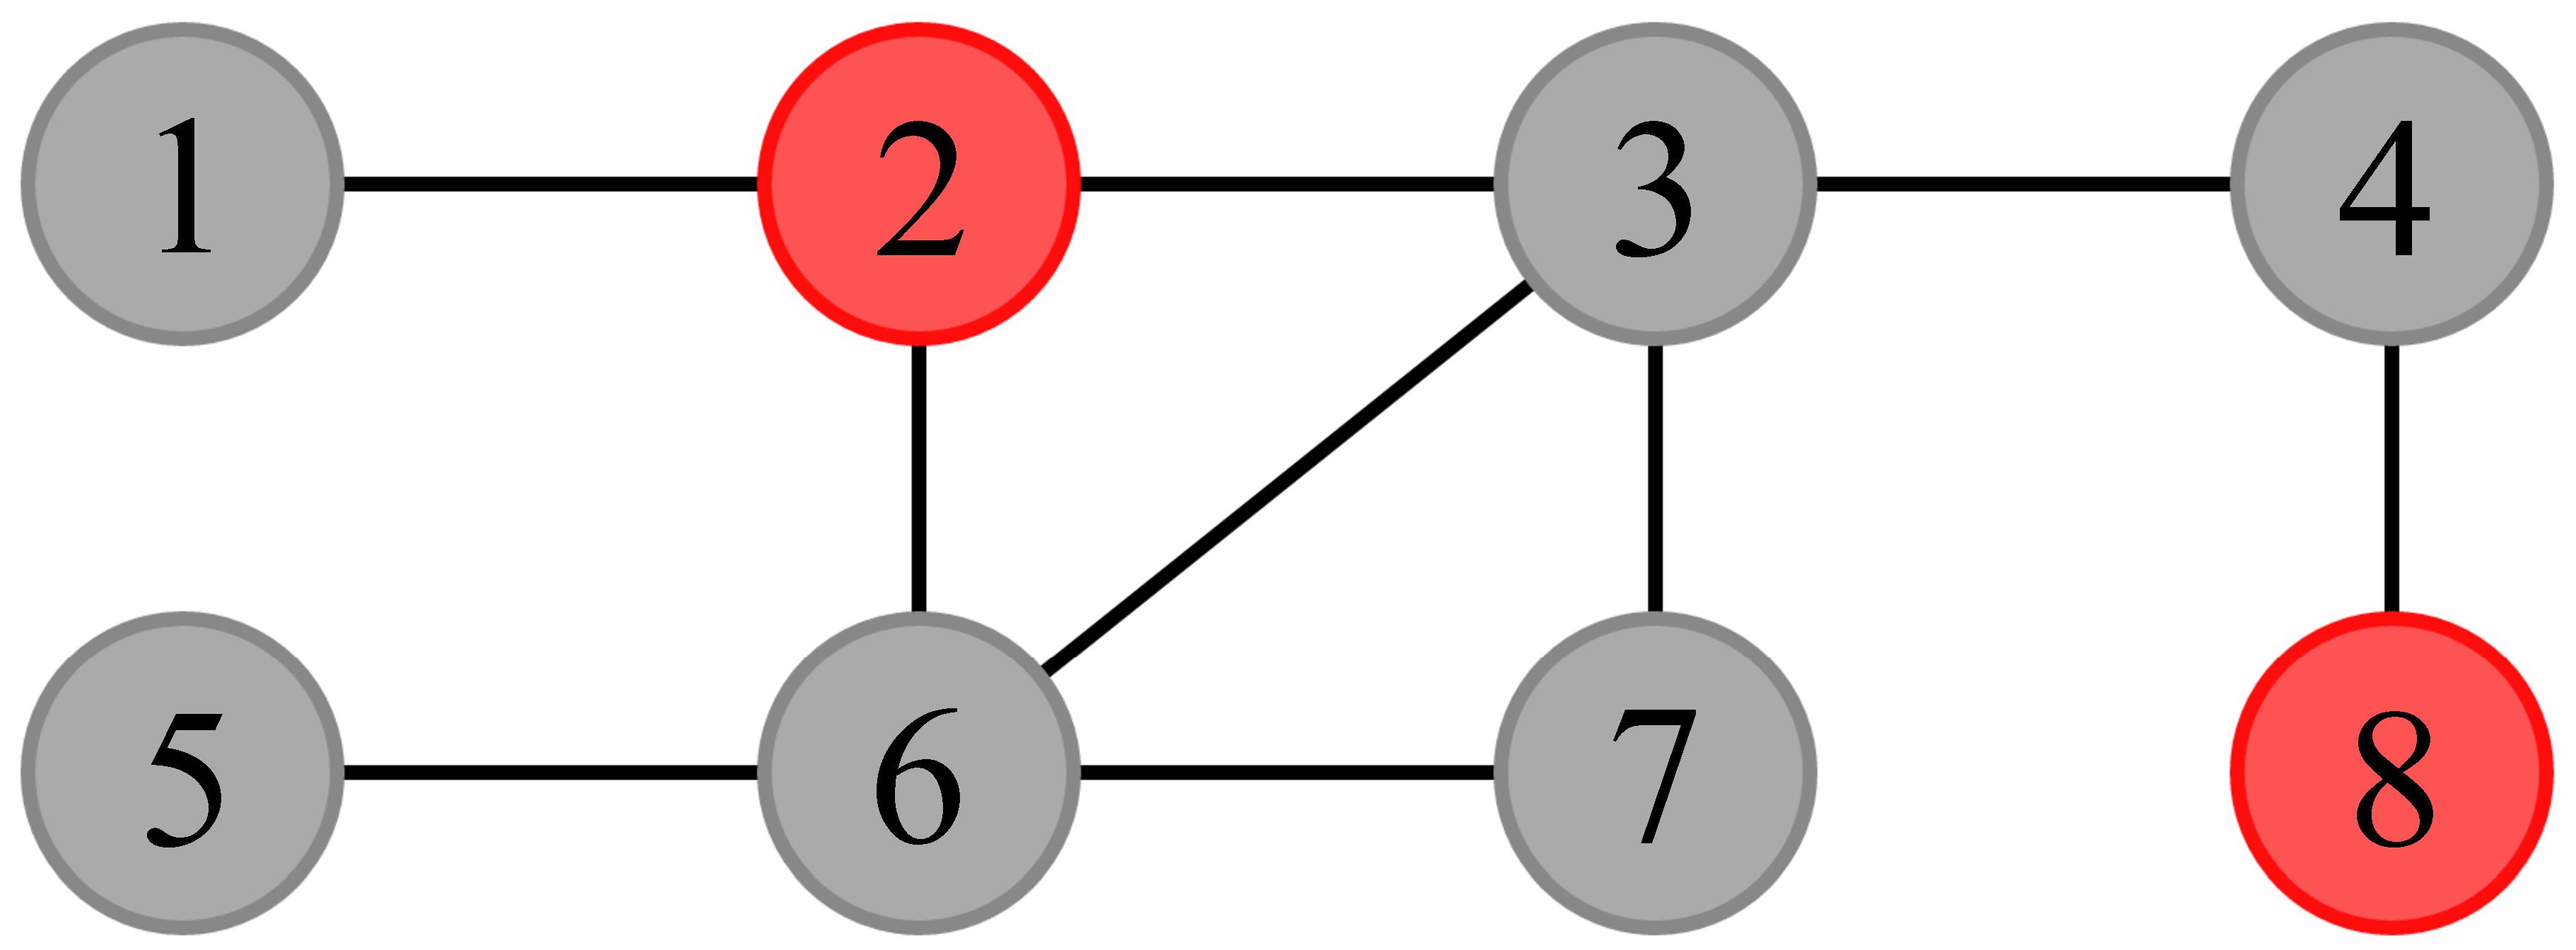
\includegraphics[width=5.7cm]{../figures/algorithm1-step1.pdf}
            \caption*{Coloring of $G$ so far}
          \end{figure}
        \end{textblock*}
        \begin{textblock*}{8cm}(8cm, 4cm) % {block width} (coords)
          \begin{figure}
            \centering
            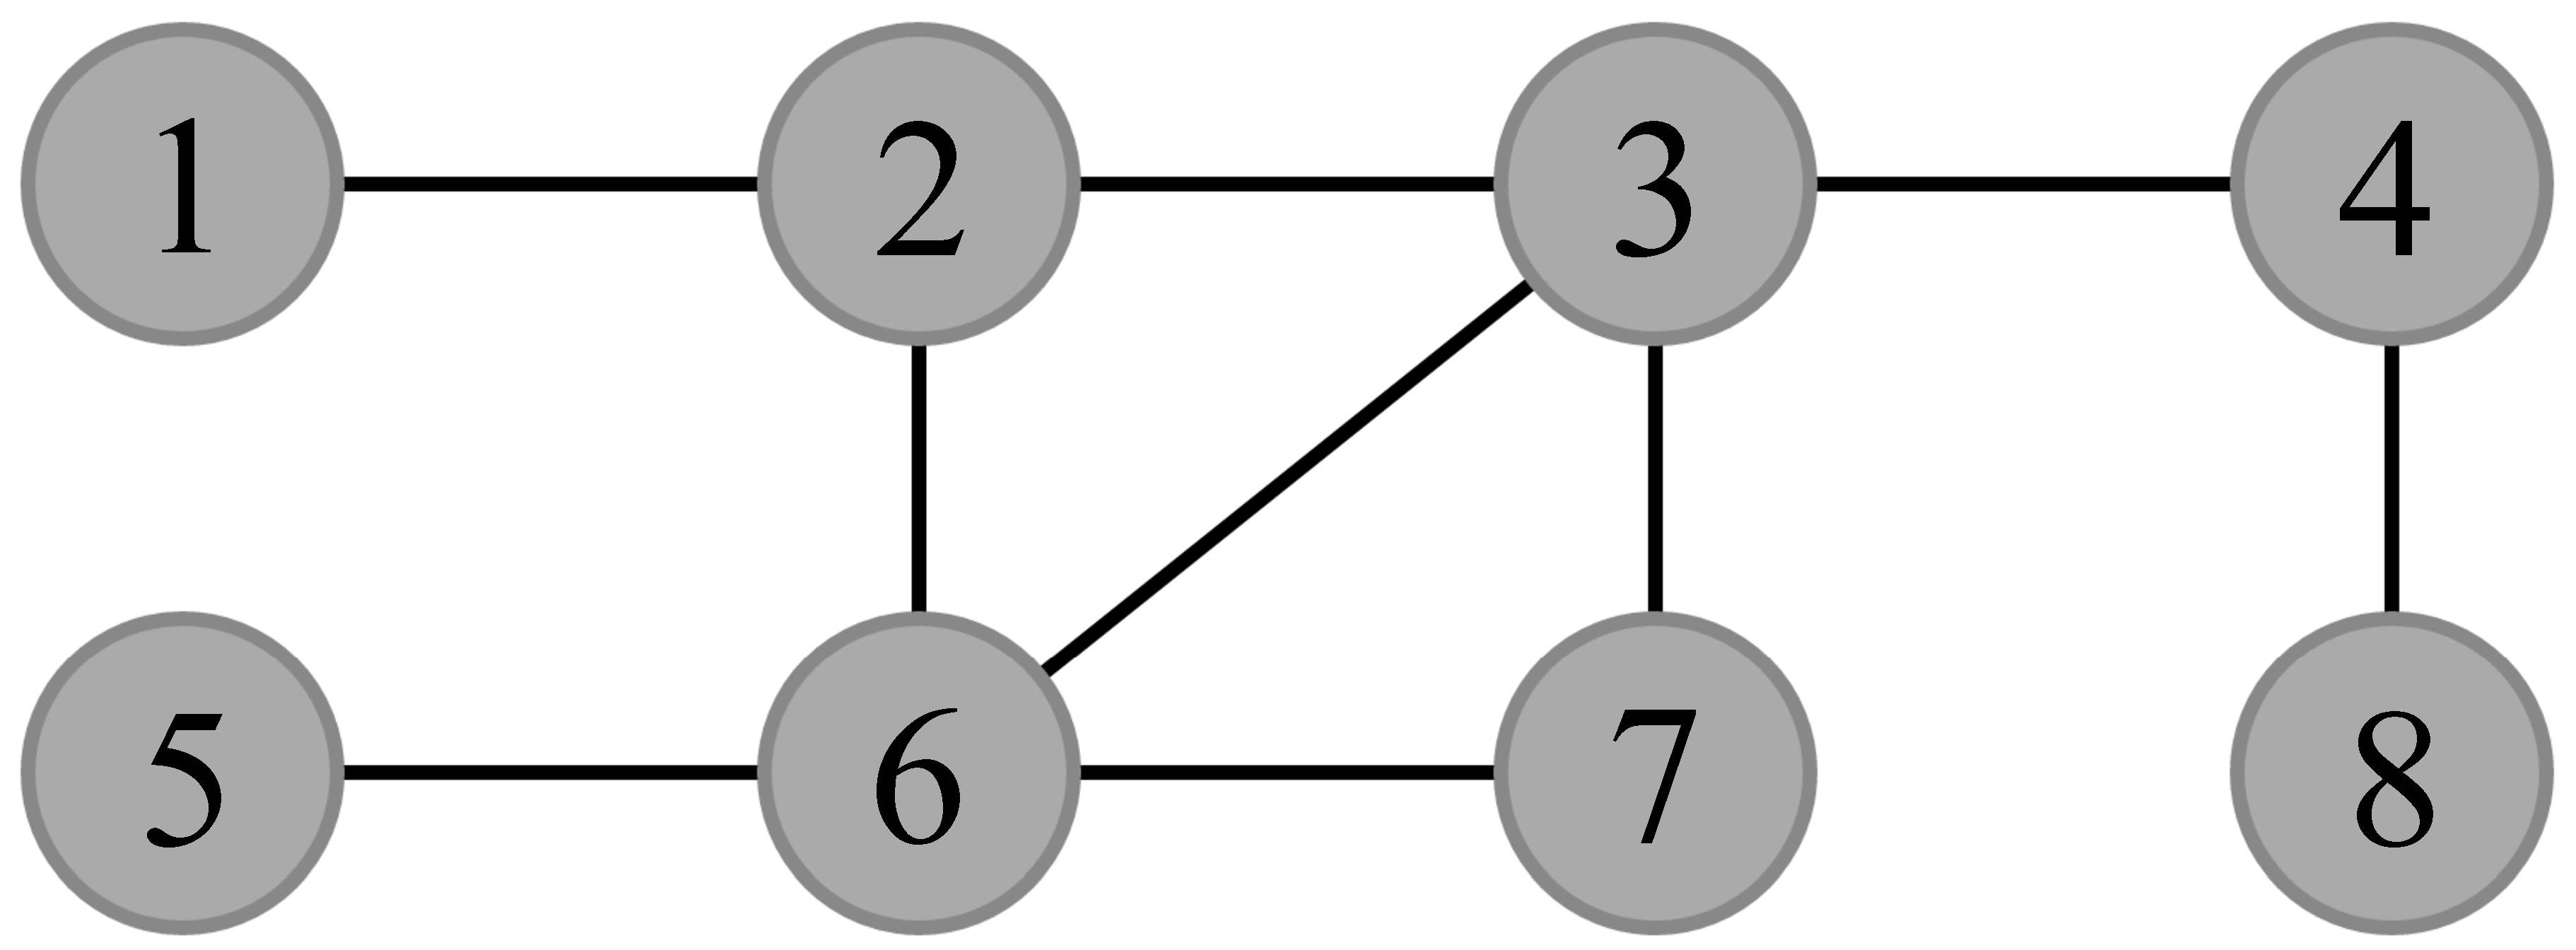
\includegraphics[width=5.7cm]{../figures/algorithm1.pdf}
            \caption*{A simple graph $G$}
          \end{figure}
        \end{textblock*}
      \end{center}
    \end{column}
  \end{columns}
}

\only<10>{
  \begin{textblock*}{8cm}(8cm, 8cm) % {block width} (coords)
    \begin{center}
      $D= \{2,8\}$
    \end{center}
  \end{textblock*}

  \begin{columns}
    \begin{column}{0.5\textwidth}
      \begin{algorithm}[H]
        \caption*{\textbf{Algorithm} IEDS}
        \scriptsize
        \begin{algorithmic}[1]
        \State $i \gets 1,\ P \gets \emptyset$
        \State Remove all isolated paths from $G$
        \While{$G$ is not empty}
          \State $D \gets \emptyset$
          \ForAll{components of $G$}
            \State Pick any vertex $v$
            \State $D \gets D \cup \{ v \}$
            \While{$\exists u$ at distance $\geq 3$ $\forall v \in D$}
              \State Pick $u$ at distance 3 from some vertex in $D$
              \State $D \gets D \cup \{ w \}$
            \EndWhile
            \ForAll{$u \in D$}
              \State Color $u$ with color $i$
            \EndFor
            \State $i \gets i + 1$
            \CForAll{$u \in D$}
              \CSTATE Remove $N(u)$ from $G$
            \EndFor
            \State Remove all isolated paths from G
          \EndFor
        \EndWhile
        \State Color all removed isolated paths using color $i$
        \end{algorithmic}
      \end{algorithm}
    \end{column}
    \begin{column}{0.5\textwidth}
      \begin{center}
        \begin{textblock*}{8cm}(8cm, 1.2cm) % {block width} (coords)
          \begin{figure}
            \centering
            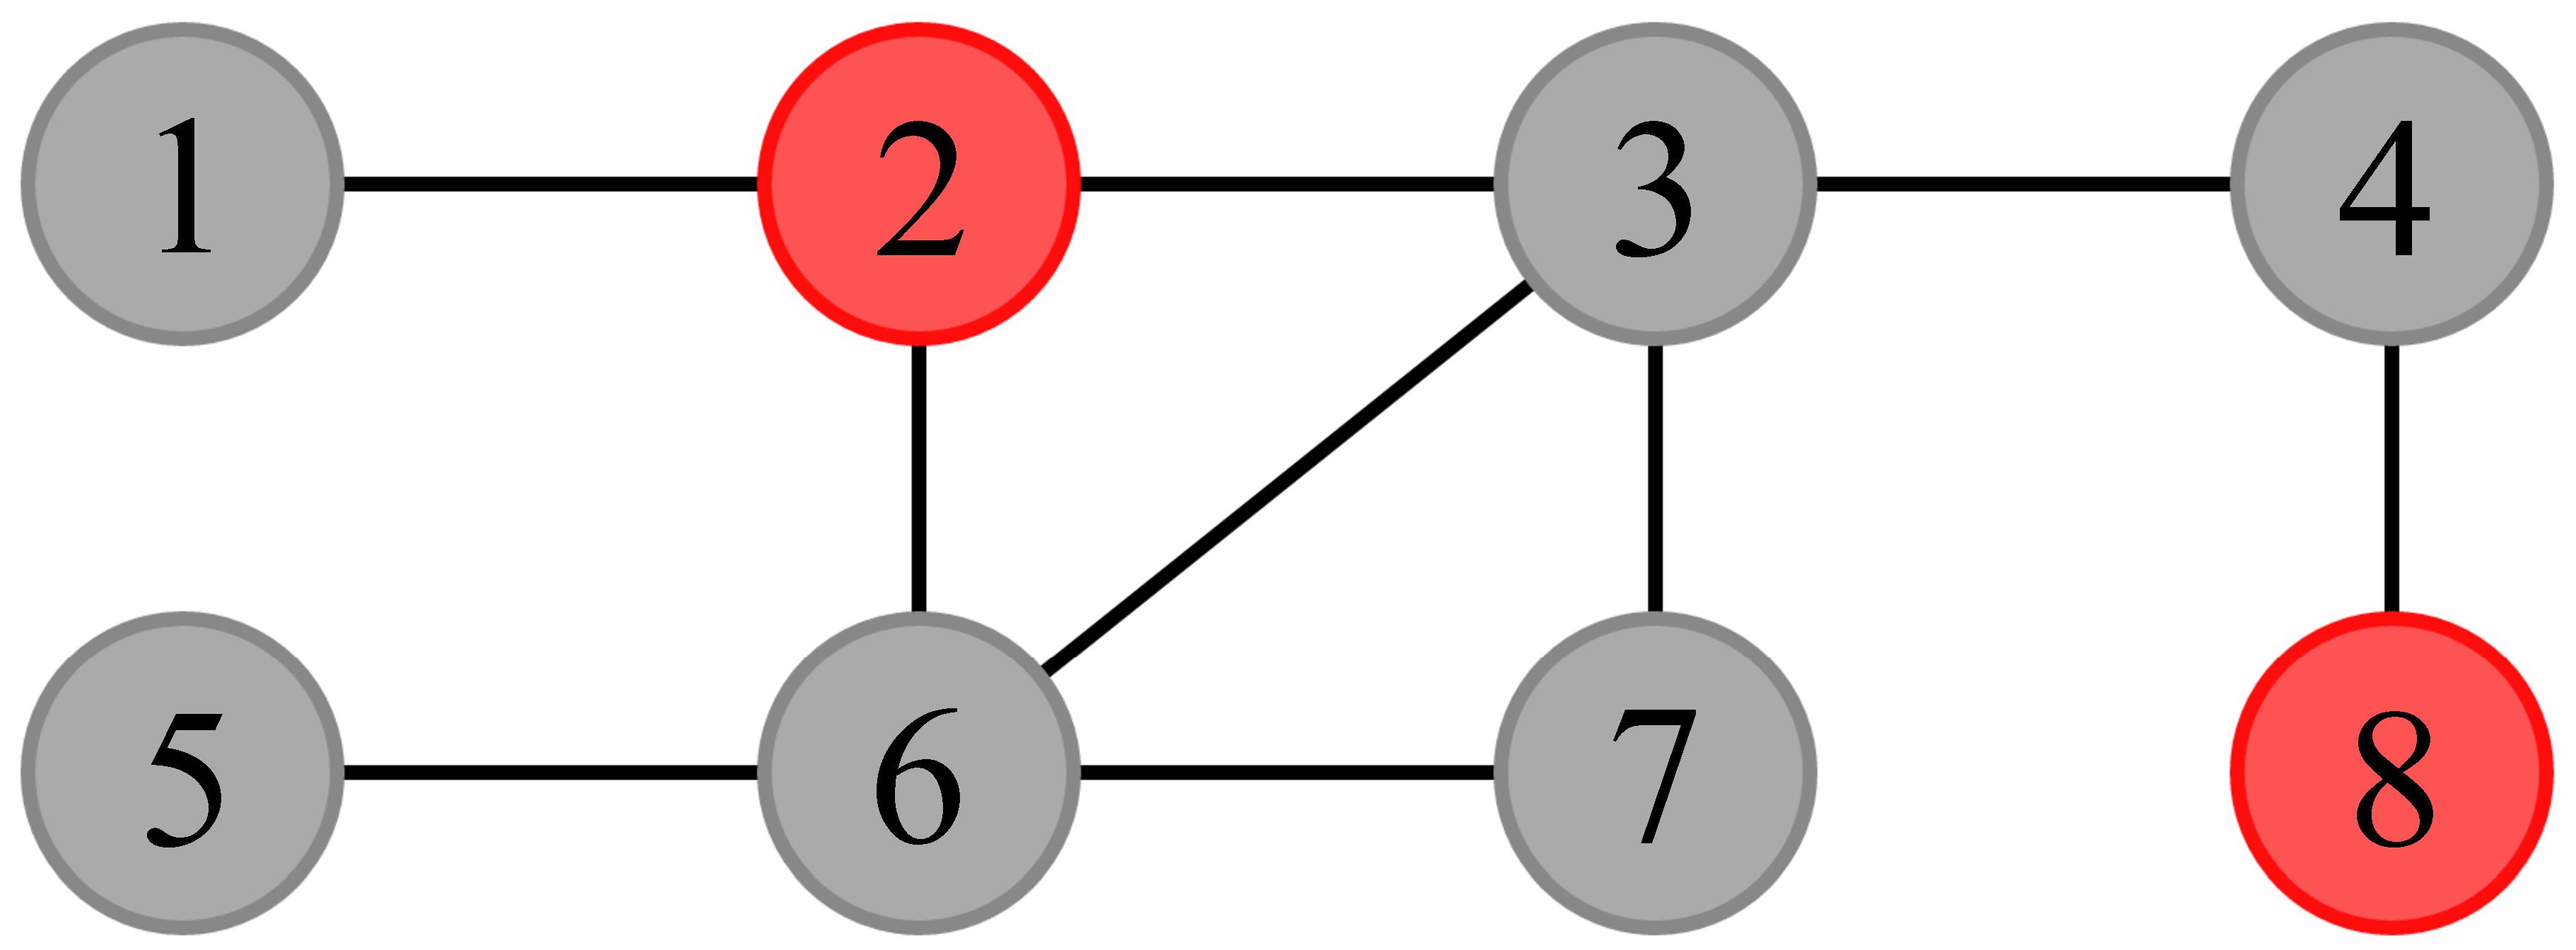
\includegraphics[width=5.7cm]{../figures/algorithm1-step1.pdf}
            \caption*{Coloring of $G$ so far}
          \end{figure}
        \end{textblock*}
        \begin{textblock*}{8cm}(8cm, 4.5cm) % {block width} (coords)
          \begin{figure}
            \centering
            
\includegraphics[width=3.5cm]{../figures/algorithm1-slide-4.pdf}
            \caption*{A simple graph $G$}
          \end{figure}
        \end{textblock*}
      \end{center}
    \end{column}
  \end{columns}
}

\only<11>{
  \begin{textblock*}{8cm}(8cm, 8cm) % {block width} (coords)
    \begin{center}
      $D= \{2,8\}$
    \end{center}
  \end{textblock*}

  \begin{columns}
    \begin{column}{0.5\textwidth}
      \begin{algorithm}[H]
        \caption*{\textbf{Algorithm} IEDS}
        \scriptsize
        \begin{algorithmic}[1]
        \State $i \gets 1,\ P \gets \emptyset$
        \State Remove all isolated paths from $G$
        \While{$G$ is not empty}
          \State $D \gets \emptyset$
          \ForAll{components of $G$}
            \State Pick any vertex $v$
            \State $D \gets D \cup \{ v \}$
            \While{$\exists u$ at distance $\geq 3$ $\forall v \in D$}
              \State Pick $u$ at distance 3 from some vertex in $D$
              \State $D \gets D \cup \{ w \}$
            \EndWhile
            \ForAll{$u \in D$}
              \State Color $u$ with color $i$
            \EndFor
            \State $i \gets i + 1$
            \ForAll{$u \in D$}
              \State Remove $N(u)$ from $G$
            \EndFor
            \CSTATE Remove all isolated paths from G
          \EndFor
        \EndWhile
        \State Color all removed isolated paths using color $i$
        \end{algorithmic}
      \end{algorithm}
    \end{column}
    \begin{column}{0.5\textwidth}
      \begin{center}
        \begin{textblock*}{8cm}(8cm, 1.2cm) % {block width} (coords)
          \begin{figure}
            \centering
            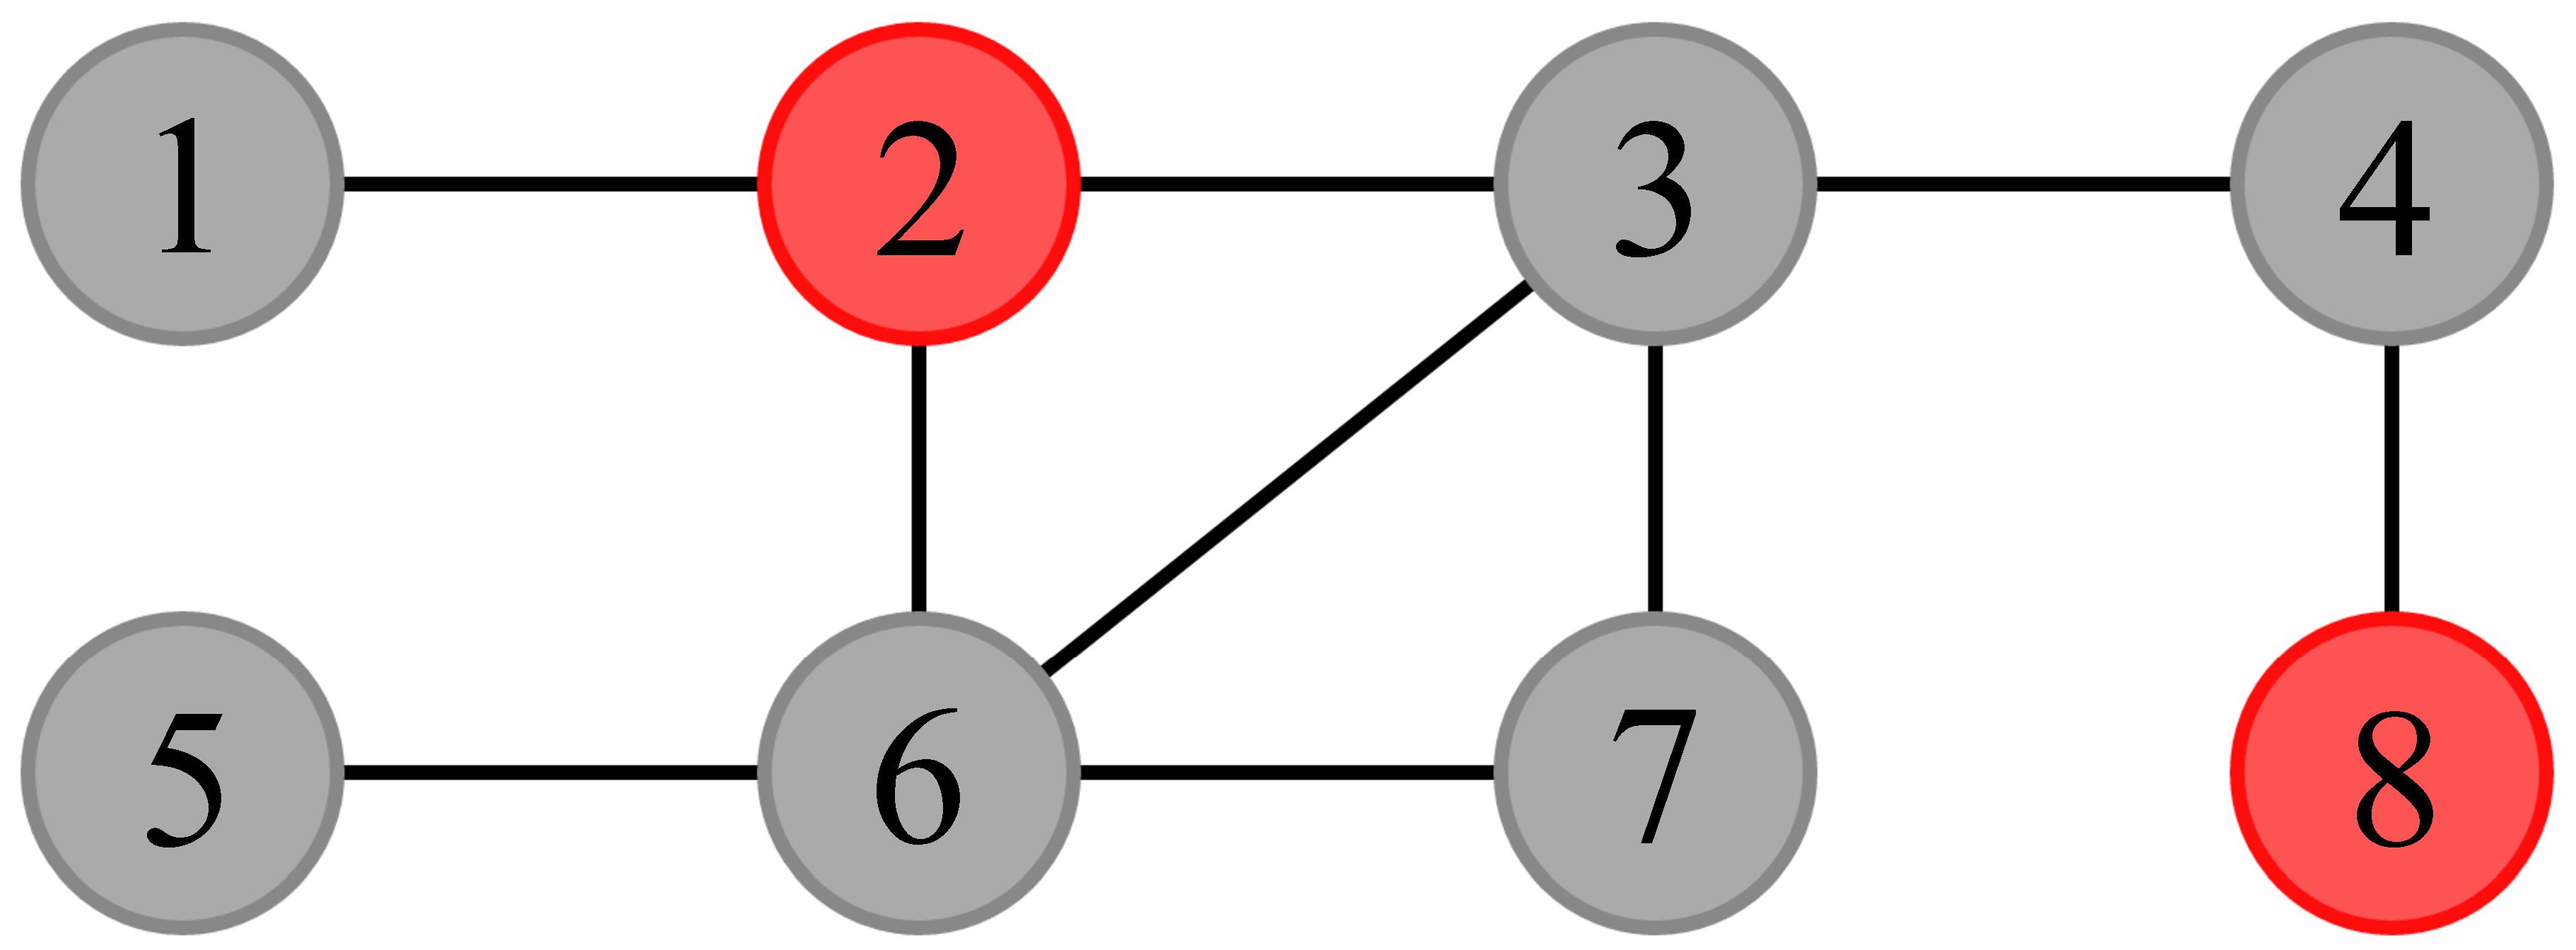
\includegraphics[width=5.7cm]{../figures/algorithm1-step1.pdf}
            \caption*{Coloring of $G$ so far}
          \end{figure}
        \end{textblock*}
        \begin{textblock*}{8cm}(8cm, 5cm) % {block width} (coords)
          \begin{figure}
            \centering
            \caption*{$G$ is now empty}
          \end{figure}
        \end{textblock*}
      \end{center}
    \end{column}
  \end{columns}
}

\only<12>{
  \begin{textblock*}{8cm}(8cm, 8cm) % {block width} (coords)
    \begin{center}
      $D= \{2,8\}$
    \end{center}
  \end{textblock*}

  \begin{columns}
    \begin{column}{0.5\textwidth}
      \begin{algorithm}[H]
        \caption*{\textbf{Algorithm} IEDS}
        \scriptsize
        \begin{algorithmic}[1]
        \State $i \gets 1,\ P \gets \emptyset$
        \State Remove all isolated paths from $G$
        \While{$G$ is not empty}
          \State $D \gets \emptyset$
          \ForAll{components of $G$}
            \State Pick any vertex $v$
            \State $D \gets D \cup \{ v \}$
            \While{$\exists u$ at distance $\geq 3$ $\forall v \in D$}
              \State Pick $u$ at distance 3 from some vertex in $D$
              \State $D \gets D \cup \{ w \}$
            \EndWhile
            \ForAll{$u \in D$}
              \State Color $u$ with color $i$
            \EndFor
            \State $i \gets i + 1$
            \ForAll{$u \in D$}
              \State Remove $N(u)$ from $G$
            \EndFor
            \State Remove all isolated paths from G
          \EndFor
        \EndWhile
        \CSTATE Color all removed isolated paths using color $i$
        \end{algorithmic}
      \end{algorithm}
    \end{column}
    \begin{column}{0.5\textwidth}
      \begin{center}
        \begin{textblock*}{8cm}(8cm, 1.2cm) % {block width} (coords)
          \begin{figure}
            \centering
            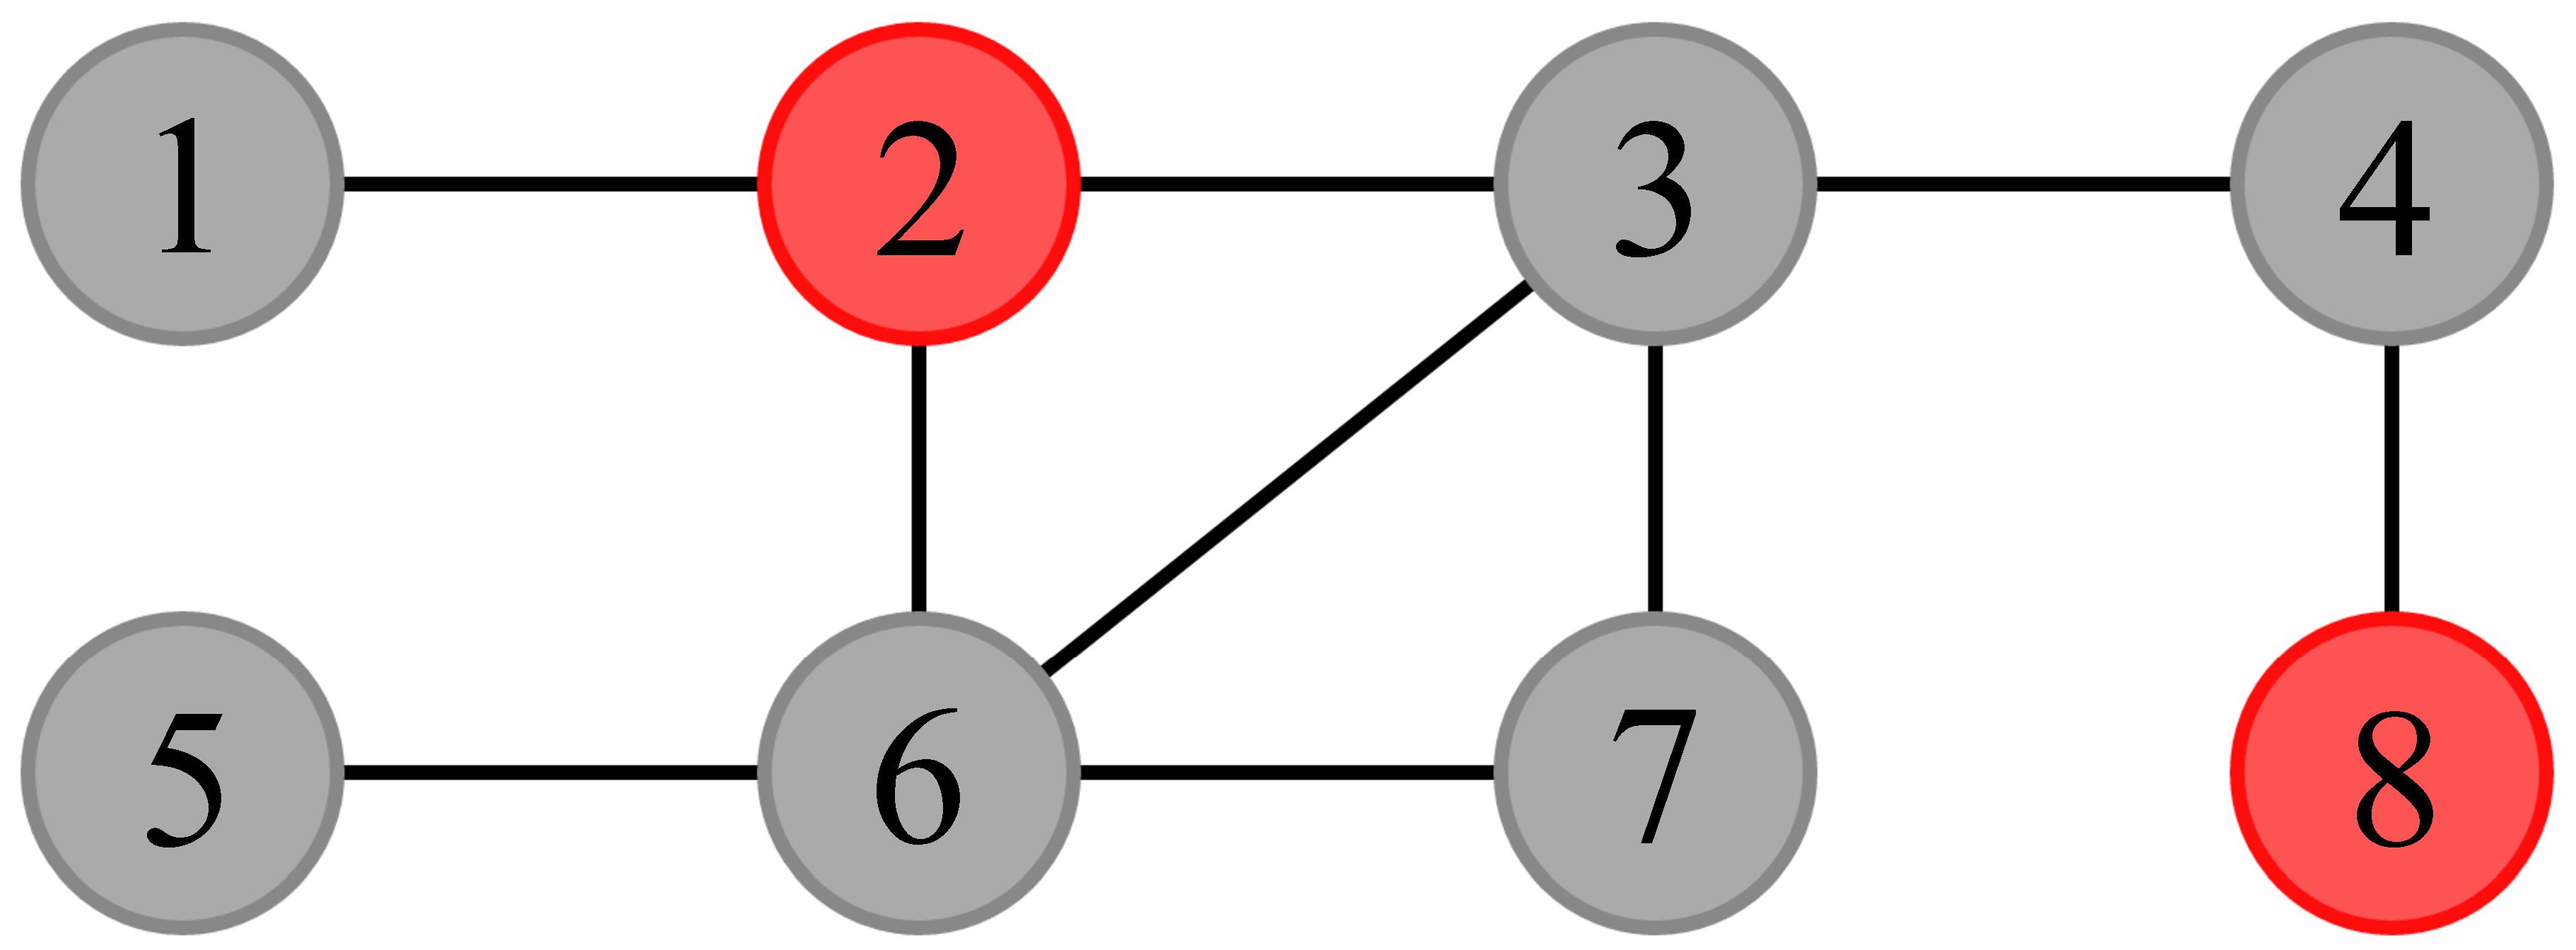
\includegraphics[width=5.7cm]{../figures/algorithm1-step1.pdf}
            \caption*{Coloring of $G$ so far}
          \end{figure}
        \end{textblock*}
        \begin{textblock*}{8cm}(8cm, 4.5cm) % {block width} (coords)
          \begin{figure}
            \centering
            
\includegraphics[width=3.5cm]{../figures/algorithm1-slide-5.pdf}
            \caption*{Coloring removed isolated paths}
          \end{figure}
        \end{textblock*}
      \end{center}
    \end{column}
  \end{columns}
}

\only<13>{
  \begin{textblock*}{8cm}(8cm, 8cm) % {block width} (coords)
    \begin{center}
      $D= \{2,8\}$
    \end{center}
  \end{textblock*}

  \begin{columns}
    \begin{column}{0.5\textwidth}
      \begin{algorithm}[H]
        \caption*{\textbf{Algorithm} IEDS}
        \scriptsize
        \begin{algorithmic}[1]
        \State $i \gets 1,\ P \gets \emptyset$
        \State Remove all isolated paths from $G$
        \While{$G$ is not empty}
          \State $D \gets \emptyset$
          \ForAll{components of $G$}
            \State Pick any vertex $v$
            \State $D \gets D \cup \{ v \}$
            \While{$\exists u$ at distance $\geq 3$ $\forall v \in D$}
              \State Pick $u$ at distance 3 from some vertex in $D$
              \State $D \gets D \cup \{ w \}$
            \EndWhile
            \ForAll{$u \in D$}
              \State Color $u$ with color $i$
            \EndFor
            \State $i \gets i + 1$
            \ForAll{$u \in D$}
              \State Remove $N(u)$ from $G$
            \EndFor
            \State Remove all isolated paths from G
          \EndFor
        \EndWhile
        \State Color all removed isolated paths using color $i$
        \end{algorithmic}
      \end{algorithm}
    \end{column}
    \begin{column}{0.5\textwidth}
      \begin{center}
        \begin{textblock*}{8cm}(8cm, 1.2cm) % {block width} (coords)
          \begin{figure}
            \centering
            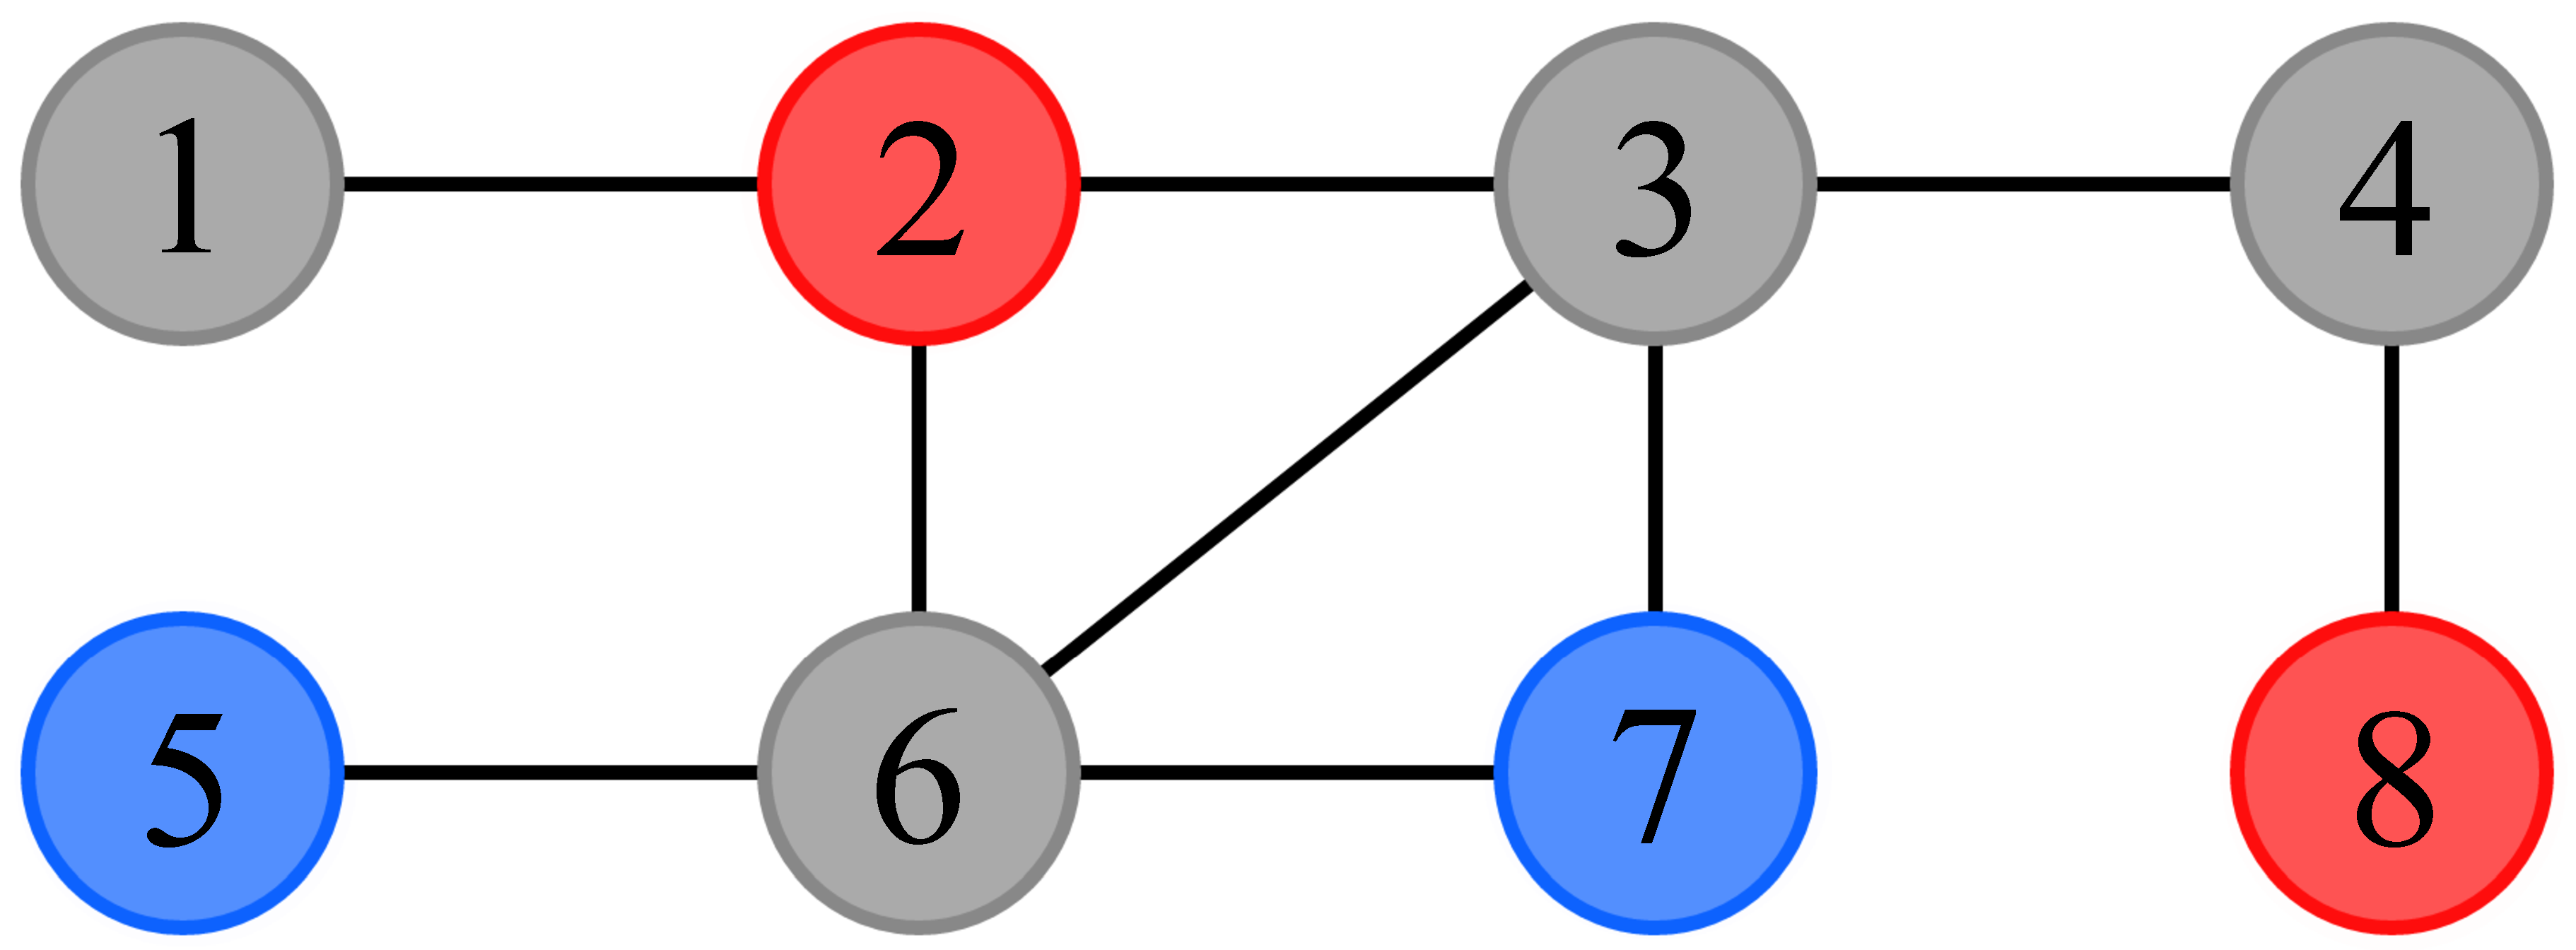
\includegraphics[width=5.7cm]{../figures/algorithm1-step3.pdf}
            \caption*{Final coloring of $G$}
          \end{figure}
        \end{textblock*}

      \end{center}
    \end{column}
  \end{columns}
}


  \end{frame}

  \addtocontents{toc}{\protect\vspace{7pt}}

  \section{Coloring for Planar Graphs}

  \subsection{Bounds for Planar Graphs}
  \begin{frame}
    \frametitle{Bounds on Planar Graphs}

    \only<3>{
      \begin{figure}[h]
        \centering
        \includegraphics[width=8cm,trim=4 4 4 4,clip]{../figures/four.pdf}
        \caption*{A vertex and conflict-free coloring, respectively}
      \end{figure}
    }

    \begin{theorem}
    Every loopless planar graph admits a proper \textbf{vertex coloring} with at most {\color{red} four} distinct colors.
    \end{theorem}

    \pause

    \begin{theorem}
    Every loopless planar graph admits a \textbf{conflict-free coloring} with at most {\color{red} three} distinct colors.
    \end{theorem}

  \end{frame}

  \subsection{Dominating Set Algorithm}
  \begin{frame}
    \frametitle{Conflict-Free Coloring via Dominating Set}

    \begin{textblock*}{8cm}(8cm, 6cm) % {block width} (coords)
  \begin{center}
    \only<2-12>{
      $D = \{2, 6, 8\}$
    }
  \end{center}
\end{textblock*}

\begin{textblock*}{8cm}(8cm, 6.5cm) % {block width} (coords)
  \begin{center}
    \only<3-4>{
      $V \setminus D = \{1, 3, 4, 5, 7\}$
    }

    \only<5-7>{
      $V \setminus D = \{3, 4, 5, 7\}$
    }

    \only<8>{
      $V \setminus D = \{4, 5, 7\}$
    }

    \only<9-12>{
      $V \setminus D = \{\}$
    }
  \end{center}
\end{textblock*}

\begin{textblock*}{8cm}(8cm,7cm) % {block width} (coords)
  \begin{center}
    \only<3-5>{
      $v \in V \setminus D = 1$
    }

    \only<6-7>{
      $v \in V \setminus D = 3$
    }
  \end{center}
\end{textblock*}

\begin{textblock*}{8cm}(8cm,7.5cm) % {block width} (coords)
  \begin{center}
    \only<4>{
      $u \in D = 2, \{1, 2\} \in E$
    }

    \only<7>{
      $u \in D = 2, \{2, 3\} \in E$
    }
  \end{center}
\end{textblock*}

\only<1>{
  \begin{columns}
    \begin{column}{0.5\textwidth}
      \begin{algorithm}[H]
        \caption*{\textbf{Algorithm} Dominating Set}
        \footnotesize
        \begin{algorithmic}[1]
        \State Find a dominating set, $D$, of $G$
        \ForAll{$v \in V \setminus D$}
        	\State Pick a vertex $u \in D$ where $\{u, v\} \in E$
        	\State Contract the edge $\{u,v\}$ towards $u$
        \EndFor
        \State Find a proper vertex coloring of $G$
        \State Color the original $G$ with the found coloring
        \end{algorithmic}
      \end{algorithm}
    \end{column}
    \begin{column}{0.5\textwidth}
      \begin{center}
        \begin{textblock*}{8cm}(8cm, 2cm) % {block width} (coords)
          \begin{figure}
            \centering
            \includegraphics[width=6cm]{../figures/algorithm1.pdf}
            \caption*{A simple, undirected graph $G = (V, E)$}
          \end{figure}
        \end{textblock*}
      \end{center}
    \end{column}
  \end{columns}
}

\only<2>{
  \begin{columns}
    \begin{column}{0.5\textwidth}
      \begin{algorithm}[H]
        \caption*{\textbf{Algorithm} Dominating Set}
        \footnotesize
        \begin{algorithmic}[1]
        \CSTATE Find a dominating set, $D$, of $G$
        \ForAll{$v \in V \setminus D$}
        	\State Pick a vertex $u \in D$ where $\{u, v\} \in E$
        	\State Contract the edge $\{u,v\}$ towards $u$
        \EndFor
        \State Find a proper vertex coloring of $G$
        \State Color the original $G$ with the found coloring
        \end{algorithmic}
      \end{algorithm}
    \end{column}
    \begin{column}{0.5\textwidth}
      \begin{center}
        \begin{textblock*}{8cm}(8cm, 2cm) % {block width} (coords)
          \begin{figure}
            \centering
            \includegraphics[width=6cm]{../figures/algorithm2-slide-1.pdf}
            \caption*{A dominating set of $G$}
          \end{figure}
        \end{textblock*}
      \end{center}
    \end{column}
  \end{columns}
}

\only<3>{
  \begin{columns}
    \begin{column}{0.5\textwidth}
      \begin{algorithm}[H]
        \caption*{\textbf{Algorithm} Dominating Set}
        \footnotesize
        \begin{algorithmic}[1]
        \State Find a dominating set, $D$, of $G$
        \CForAll{$v \in V \setminus D$}
        	\State Pick a vertex $u \in D$ where $\{u, v\} \in E$
        	\State Contract the edge $\{u,v\}$ towards $u$
        \EndFor
        \State Find a proper vertex coloring of $G$
        \State Color the original $G$ with the found coloring
        \end{algorithmic}
      \end{algorithm}
    \end{column}
    \begin{column}{0.5\textwidth}
      \begin{center}
        \begin{textblock*}{8cm}(8cm, 2cm) % {block width} (coords)
          \begin{figure}
            \centering
            \includegraphics[width=6cm]{../figures/algorithm2-slide-2.pdf}
            \caption*{Pick $v$ to be vertex 1}
          \end{figure}
        \end{textblock*}
      \end{center}
    \end{column}
  \end{columns}
}

\only<4>{
  \begin{columns}
    \begin{column}{0.5\textwidth}
      \begin{algorithm}[H]
        \caption*{\textbf{Algorithm} Dominating Set}
        \footnotesize
        \begin{algorithmic}[1]
        \State Find a dominating set, $D$, of $G$
        \ForAll{$v \in V \setminus D$}
        	\CSTATE Pick a vertex $u \in D$ where $\{u, v\} \in E$
        	\State Contract the edge $\{u,v\}$ towards $u$
        \EndFor
        \State Find a proper vertex coloring of $G$
        \State Color the original $G$ with the found coloring
        \end{algorithmic}
      \end{algorithm}
    \end{column}
    \begin{column}{0.5\textwidth}
      \begin{center}
        \begin{textblock*}{8cm}(8cm, 2cm) % {block width} (coords)
          \begin{figure}
            \centering
            \includegraphics[width=6cm]{../figures/algorithm2-slide-4.pdf}
            \caption*{Pick $u$ to be vertex 2}
          \end{figure}
        \end{textblock*}
      \end{center}
    \end{column}
  \end{columns}
}

\only<5>{
  \begin{columns}
    \begin{column}{0.5\textwidth}
      \begin{algorithm}[H]
        \caption*{\textbf{Algorithm} Dominating Set}
        \footnotesize
        \begin{algorithmic}[1]
        \State Find a dominating set, $D$, of $G$
        \ForAll{$v \in V \setminus D$}
        	\State Pick a vertex $u \in D$ where $\{u, v\} \in E$
        	\CSTATE Contract the edge $\{u,v\}$ towards $u$
        \EndFor
        \State Find a proper vertex coloring of $G$
        \State Color the original $G$ with the found coloring
        \end{algorithmic}
      \end{algorithm}
    \end{column}
    \begin{column}{0.5\textwidth}
      \begin{center}
        \begin{textblock*}{8cm}(8cm, 2cm) % {block width} (coords)
          \begin{figure}
            \centering
            \includegraphics[width=6cm]{../figures/algorithm2-slide-5.pdf}
            \caption*{Contract $\{1, 2\}$ towards 2}
          \end{figure}
        \end{textblock*}
      \end{center}
    \end{column}
  \end{columns}
}

\only<6>{
  \begin{columns}
    \begin{column}{0.5\textwidth}
      \begin{algorithm}[H]
        \caption*{\textbf{Algorithm} Dominating Set}
        \footnotesize
        \begin{algorithmic}[1]
        \State Find a dominating set, $D$, of $G$
        \CForAll{$v \in V \setminus D$}
        	\State Pick a vertex $u \in D$ where $\{u, v\} \in E$
        	\State Contract the edge $\{u,v\}$ towards $u$
        \EndFor
        \State Find a proper vertex coloring of $G$
        \State Color the original $G$ with the found coloring
        \end{algorithmic}
      \end{algorithm}
    \end{column}
    \begin{column}{0.5\textwidth}
      \begin{center}
        \begin{textblock*}{8cm}(8cm, 2cm) % {block width} (coords)
          \begin{figure}
            \centering
            \includegraphics[width=6cm]{../figures/algorithm2-slide-6.pdf}
            \caption*{Pick $v$ to be vertex 3}
          \end{figure}
        \end{textblock*}
      \end{center}
    \end{column}
  \end{columns}
}

\only<7>{
  \begin{columns}
    \begin{column}{0.5\textwidth}
      \begin{algorithm}[H]
        \caption*{\textbf{Algorithm} Dominating Set}
        \footnotesize
        \begin{algorithmic}[1]
        \State Find a dominating set, $D$, of $G$
        \ForAll{$v \in V \setminus D$}
        	\CSTATE Pick a vertex $u \in D$ where $\{u, v\} \in E$
        	\State Contract the edge $\{u,v\}$ towards $u$
        \EndFor
        \State Find a proper vertex coloring of $G$
        \State Color the original $G$ with the found coloring
        \end{algorithmic}
      \end{algorithm}
    \end{column}
    \begin{column}{0.5\textwidth}
      \begin{center}
        \begin{textblock*}{8cm}(8cm, 2cm) % {block width} (coords)
          \begin{figure}
            \centering
            \includegraphics[width=6cm]{../figures/algorithm2-slide-7.pdf}
            \caption*{Pick $u$ to be vertex 2}
          \end{figure}
        \end{textblock*}
      \end{center}
    \end{column}
  \end{columns}
}

\only<8>{
  \begin{columns}
    \begin{column}{0.5\textwidth}
      \begin{algorithm}[H]
        \caption*{\textbf{Algorithm} Dominating Set}
        \footnotesize
        \begin{algorithmic}[1]
        \State Find a dominating set, $D$, of $G$
        \ForAll{$v \in V \setminus D$}
        	\State Pick a vertex $u \in D$ where $\{u, v\} \in E$
        	\CSTATE Contract the edge $\{u,v\}$ towards $u$
        \EndFor
        \State Find a proper vertex coloring of $G$
        \State Color the original $G$ with the found coloring
        \end{algorithmic}
      \end{algorithm}
    \end{column}
    \begin{column}{0.5\textwidth}
      \begin{center}
        \begin{textblock*}{8cm}(8cm, 2cm) % {block width} (coords)
          \begin{figure}
            \centering
            \includegraphics[width=6cm]{../figures/algorithm2-slide-8.pdf}
            \caption*{Contract $\{2, 3\}$ towards 2}
          \end{figure}
        \end{textblock*}
      \end{center}
    \end{column}
  \end{columns}
}

\only<9>{
  \begin{columns}
    \begin{column}{0.5\textwidth}
      \begin{algorithm}[H]
        \caption*{\textbf{Algorithm} Dominating Set}
        \footnotesize
        \begin{algorithmic}[1]
        \State Find a dominating set, $D$, of $G$
        \ForAll{$v \in V \setminus D$}
        	\State Pick a vertex $u \in D$ where $\{u, v\} \in E$
        	\State Contract the edge $\{u,v\}$ towards $u$
        \EndFor
        \State Find a proper vertex coloring of $G$
        \State Color the original $G$ with the found coloring
        \end{algorithmic}
      \end{algorithm}
    \end{column}
    \begin{column}{0.5\textwidth}
      \begin{center}
        \begin{textblock*}{8cm}(8cm, 3cm) % {block width} (coords)
          \begin{figure}
            \centering
            \includegraphics[width=6cm]{../figures/algorithm2-slide-9.pdf}
            \caption*{$G$ after lines 2-4}
          \end{figure}
        \end{textblock*}
      \end{center}
    \end{column}
  \end{columns}
}

\only<10>{
  \begin{columns}
    \begin{column}{0.5\textwidth}
      \begin{algorithm}[H]
        \caption*{\textbf{Algorithm} Dominating Set}
        \footnotesize
        \begin{algorithmic}[1]
        \State Find a dominating set, $D$, of $G$
        \ForAll{$v \in V \setminus D$}
        	\State Pick a vertex $u \in D$ where $\{u, v\} \in E$
        	\State Contract the edge $\{u,v\}$ towards $u$
        \EndFor
        \CSTATE Find a proper vertex coloring of $G$
        \State Color the original $G$ with the found coloring
        \end{algorithmic}
      \end{algorithm}
    \end{column}
    \begin{column}{0.5\textwidth}
      \begin{center}
        \begin{textblock*}{8cm}(8cm, 3cm) % {block width} (coords)
          \begin{figure}
            \centering
            \includegraphics[width=6cm]{../figures/algorithm2-slide-10.pdf}
            \caption*{A proper vertex coloring}
          \end{figure}
        \end{textblock*}
      \end{center}
    \end{column}
  \end{columns}
}

\only<11>{
  \begin{columns}
    \begin{column}{0.5\textwidth}
      \begin{algorithm}[H]
        \caption*{\textbf{Algorithm} Dominating Set}
        \footnotesize
        \begin{algorithmic}[1]
        \State Find a dominating set, $D$, of $G$
        \ForAll{$v \in V \setminus D$}
        	\State Pick a vertex $u \in D$ where $\{u, v\} \in E$
        	\State Contract the edge $\{u,v\}$ towards $u$
        \EndFor
        \State Find a proper vertex coloring of $G$
        \CSTATE Color the original $G$ with the found coloring
        \end{algorithmic}
      \end{algorithm}
    \end{column}
    \begin{column}{0.5\textwidth}
      \begin{center}
        \begin{textblock*}{8cm}(8cm, 2cm) % {block width} (coords)
          \begin{figure}
            \centering
            \includegraphics[width=6cm]{../figures/algorithm2-step4.pdf}
            \caption*{Original $G$ colored}
          \end{figure}
        \end{textblock*}
      \end{center}
    \end{column}
  \end{columns}
}

\only<12>{
  \begin{columns}
    \begin{column}{0.5\textwidth}
      \begin{algorithm}[H]
        \caption*{\textbf{Algorithm} Dominating Set}
        \footnotesize
        \begin{algorithmic}[1]
        \State Find a dominating set, $D$, of $G$
        \ForAll{$v \in V \setminus D$}
        	\State Pick a vertex $u \in D$ where $\{u, v\} \in E$
        	\State Contract the edge $\{u,v\}$ towards $u$
        \EndFor
        \State Find a proper vertex coloring of $G$
        \State Color the original $G$ with the found coloring
        \end{algorithmic}
      \end{algorithm}

      \vfill

      \begin{itemize}
        \item[(1)] Produces a valid conflict-free coloring
        \item[(2)] Tries to minimize the number of colored vertices
      \end{itemize}
    \end{column}
    \begin{column}{0.5\textwidth}
      \begin{center}
        \begin{textblock*}{8cm}(8cm, 2cm) % {block width} (coords)
          \begin{figure}
            \centering
            \includegraphics[width=6cm]{../figures/algorithm2-step4.pdf}
            \caption*{Original $G$ colored}
          \end{figure}
        \end{textblock*}
      \end{center}
    \end{column}
  \end{columns}
}

  \end{frame}

  \begin{frame}
    \frametitle{Future Work}

    \begin{itemize}
      \item Finding bounds and properties on specific graphs such as outerplanar graphs, interval graphs, hypergraphs, and more.
      \pause
      \vfill
      \begin{itemize}
        \item Allows for accurate estimates when applying conflict-free coloring to real-world problems.
      \end{itemize}
      \pause
      \vfill
      \item Variations of conflict-free coloring such as requiring \textbf{another} vertex to have a unique color within the neighborhood of a selected vertex.
      \pause
      \vfill
      \begin{itemize}
        \item Guiding a robot (unique color 1) to a destination (unique color 2).
      \end{itemize}
    \end{itemize}

  \end{frame}

  \begin{frame}[standout]
    \centering
    {Thanks to Peter Dolan, Elena Machkasova,

    and Peh Ng for their advice and feedback.}
    \vfill
    \href{https://github.com/devshawn/senior-seminar}{github.com/devshawn/senior-seminar}
    \vfill
    \ccbyncsa{}
  \end{frame}

\end{document}
